\documentclass{beamer}
\usepackage[utf8]{inputenc}
\usepackage[]{amsmath}
\usepackage{graphicx}
\usepackage{subcaption} % package pour faire des subfigures
\usepackage{multirow} % package pour multirow/multicolumn
\usepackage{booktabs} % package pour top/mid/bottom rule
\usepackage{tcolorbox} % toujours plus de boites
\usepackage[backend=biber]{biblatex}


\addbibresource{Biblio_dbl_quantum.bib}

%\bibliographystyle{stylename}
%\bibliography{Biblio_dbl_quantum}

\title{Mechanical and luminescence-based detection of dipolar-interactions between spins in diamond}
\author{Clément Pellet-Mary\\ Laboratoire de physique de l'ENS\\ \textit{ENS, Paris}}
\date\today

\mode<presentation> {\usetheme{Rochester}}

\begin{document}
\begin{frame}
\maketitle
\end{frame}
\begin{frame}
\includegraphics[scale=.3]{Shémas_intro}
\end{frame}
\section{NV center and Cross-Relaxations}
\begin{frame}{Outline}
\tableofcontents[currentsection]
\end{frame}
\begin{frame}{Spin Hamiltonian and orientation of the centers}
\begin{figure}
    \begin{overprint}
    \onslide<1>\centering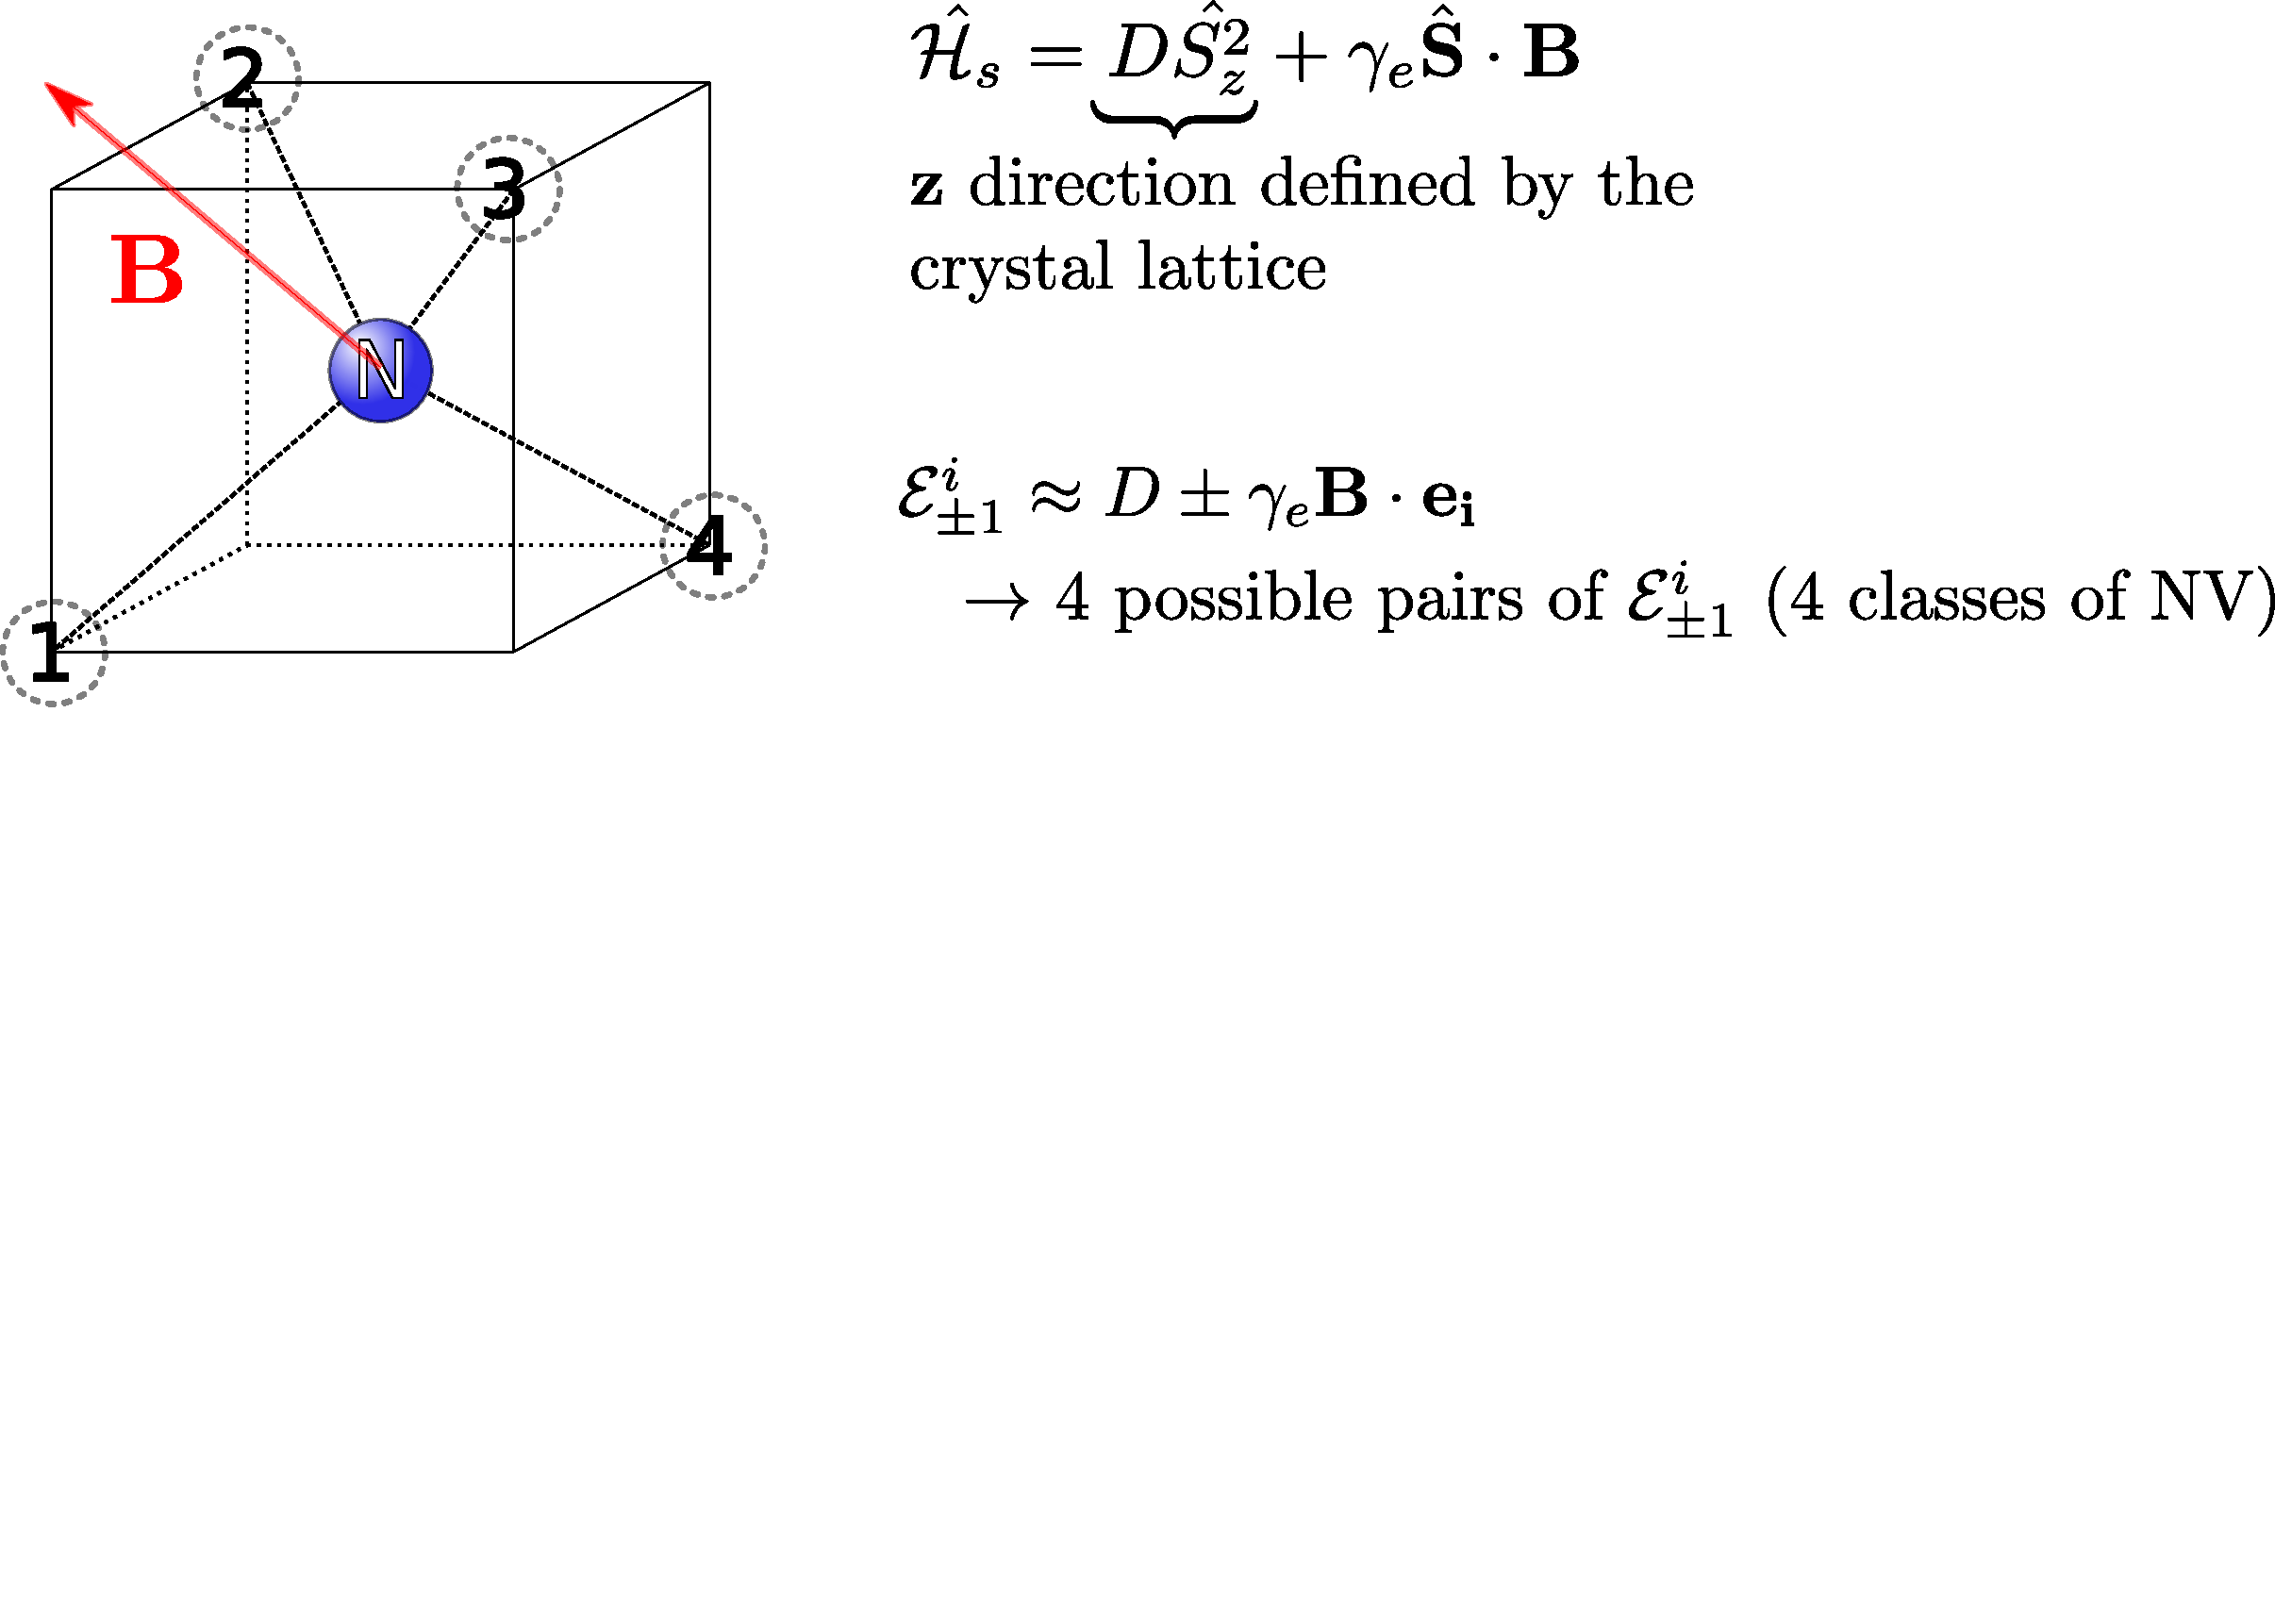
\includegraphics[scale=.25]{projection_4_classes_0}
    \onslide<2>\centering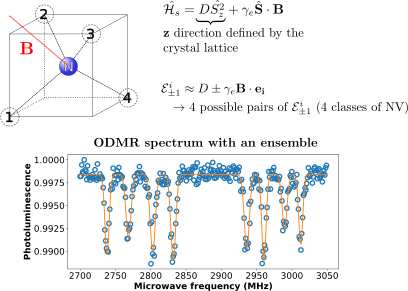
\includegraphics[scale=.25]{projection_4_classes_1}
    \end{overprint}
\end{figure}
\end{frame}
\begin{frame}{Non-Resonant dipolar interaction}
\centering
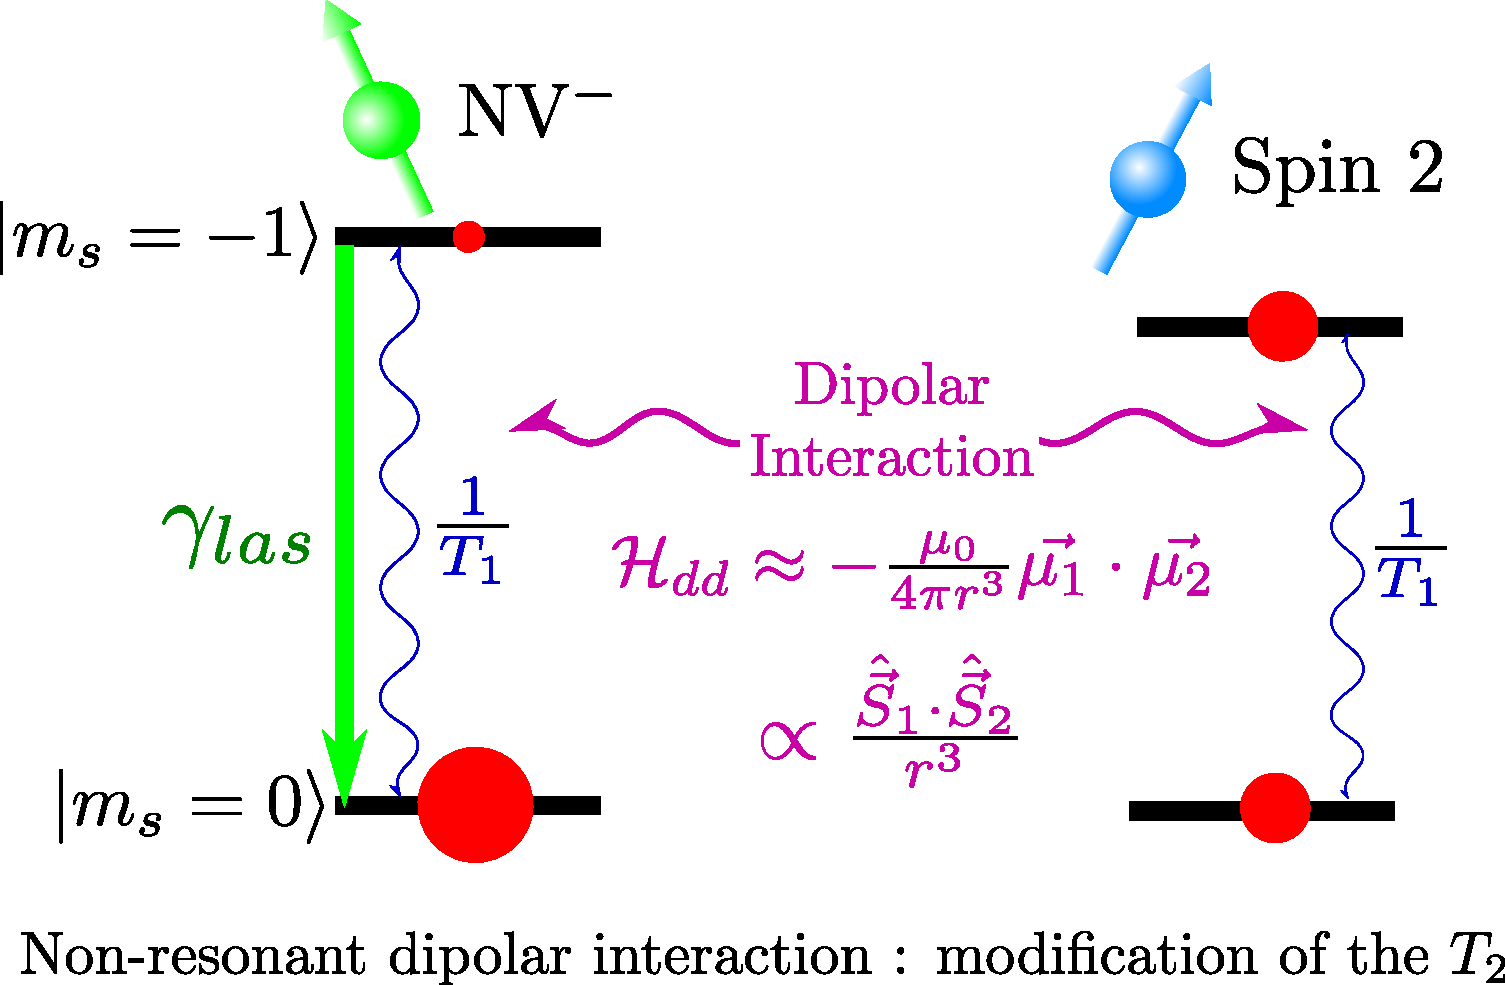
\includegraphics[scale=.35]{CR_non_resonnant}
\end{frame}
\begin{frame}{Resonant dipolar interaction : Cross-Relaxation}
\centering
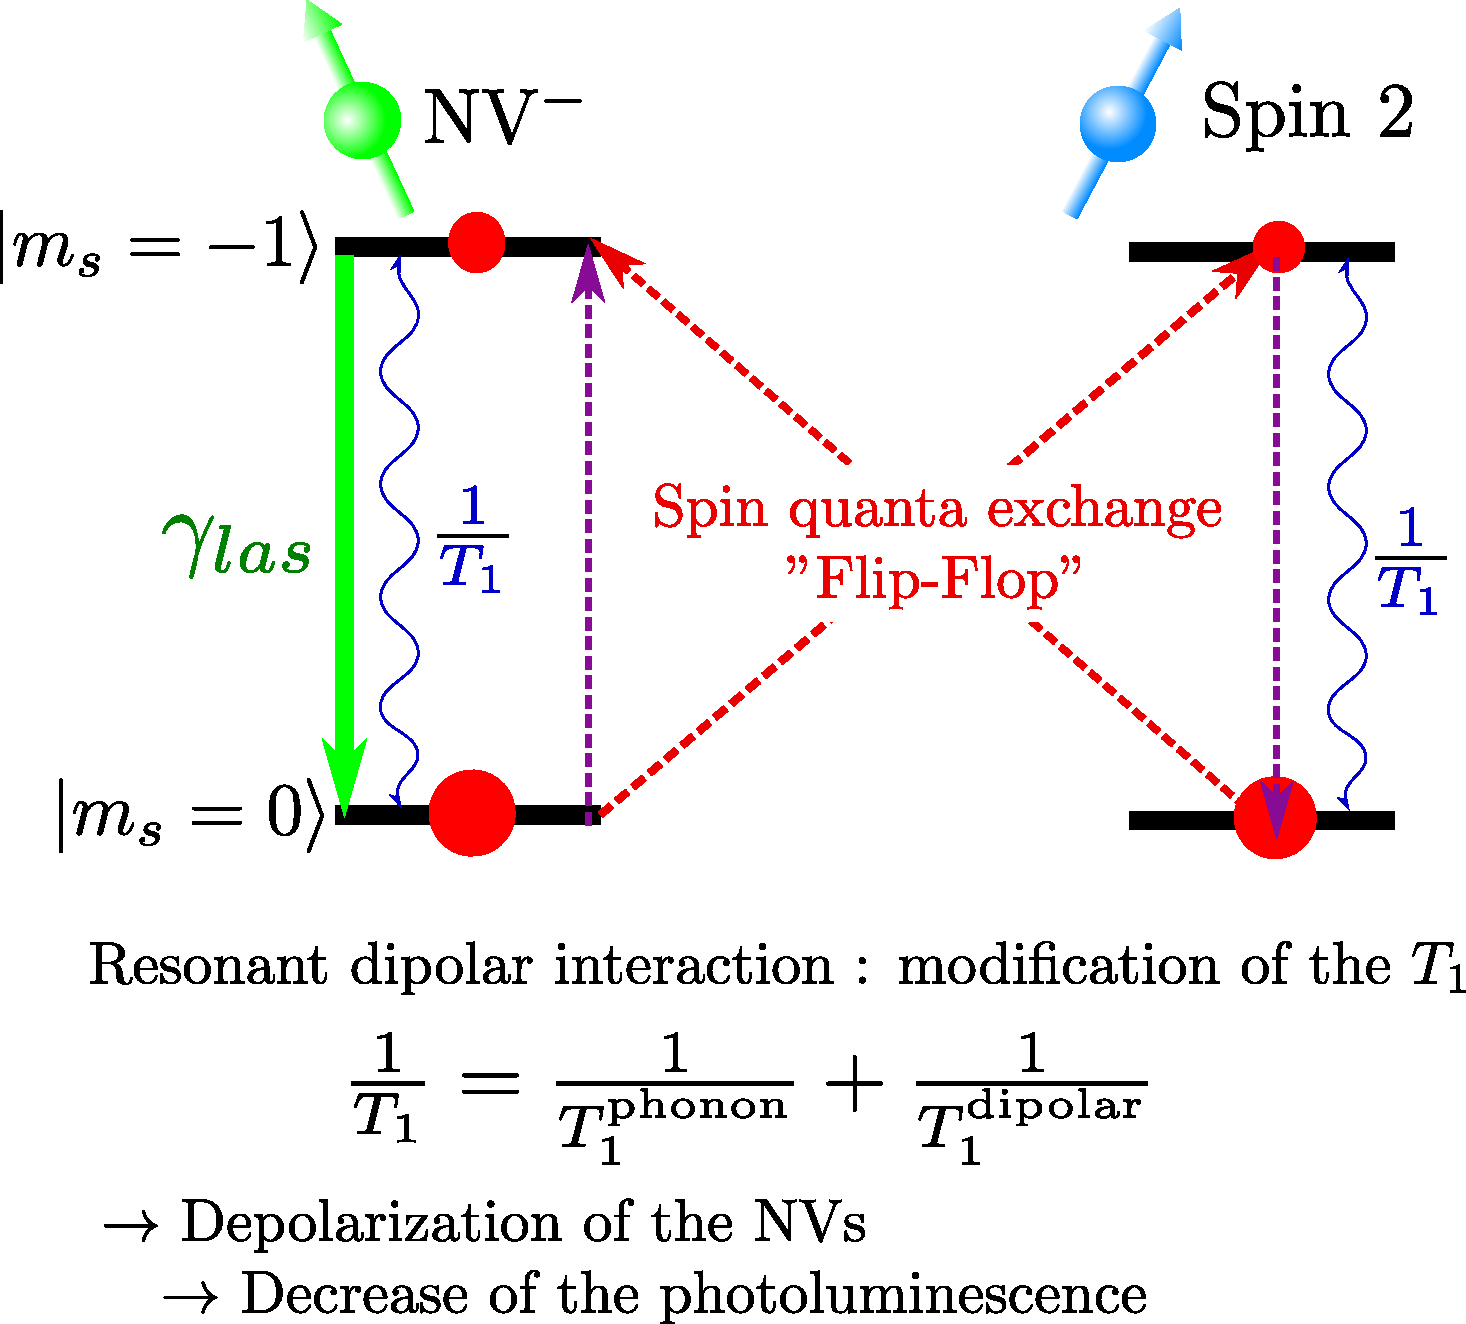
\includegraphics[scale=.35]{CR_resonnant}
\end{frame}
\begin{frame}{Exemple of Cross-Relaxation NV-P1}
\begin{figure}
    \begin{overprint}
    \onslide<1>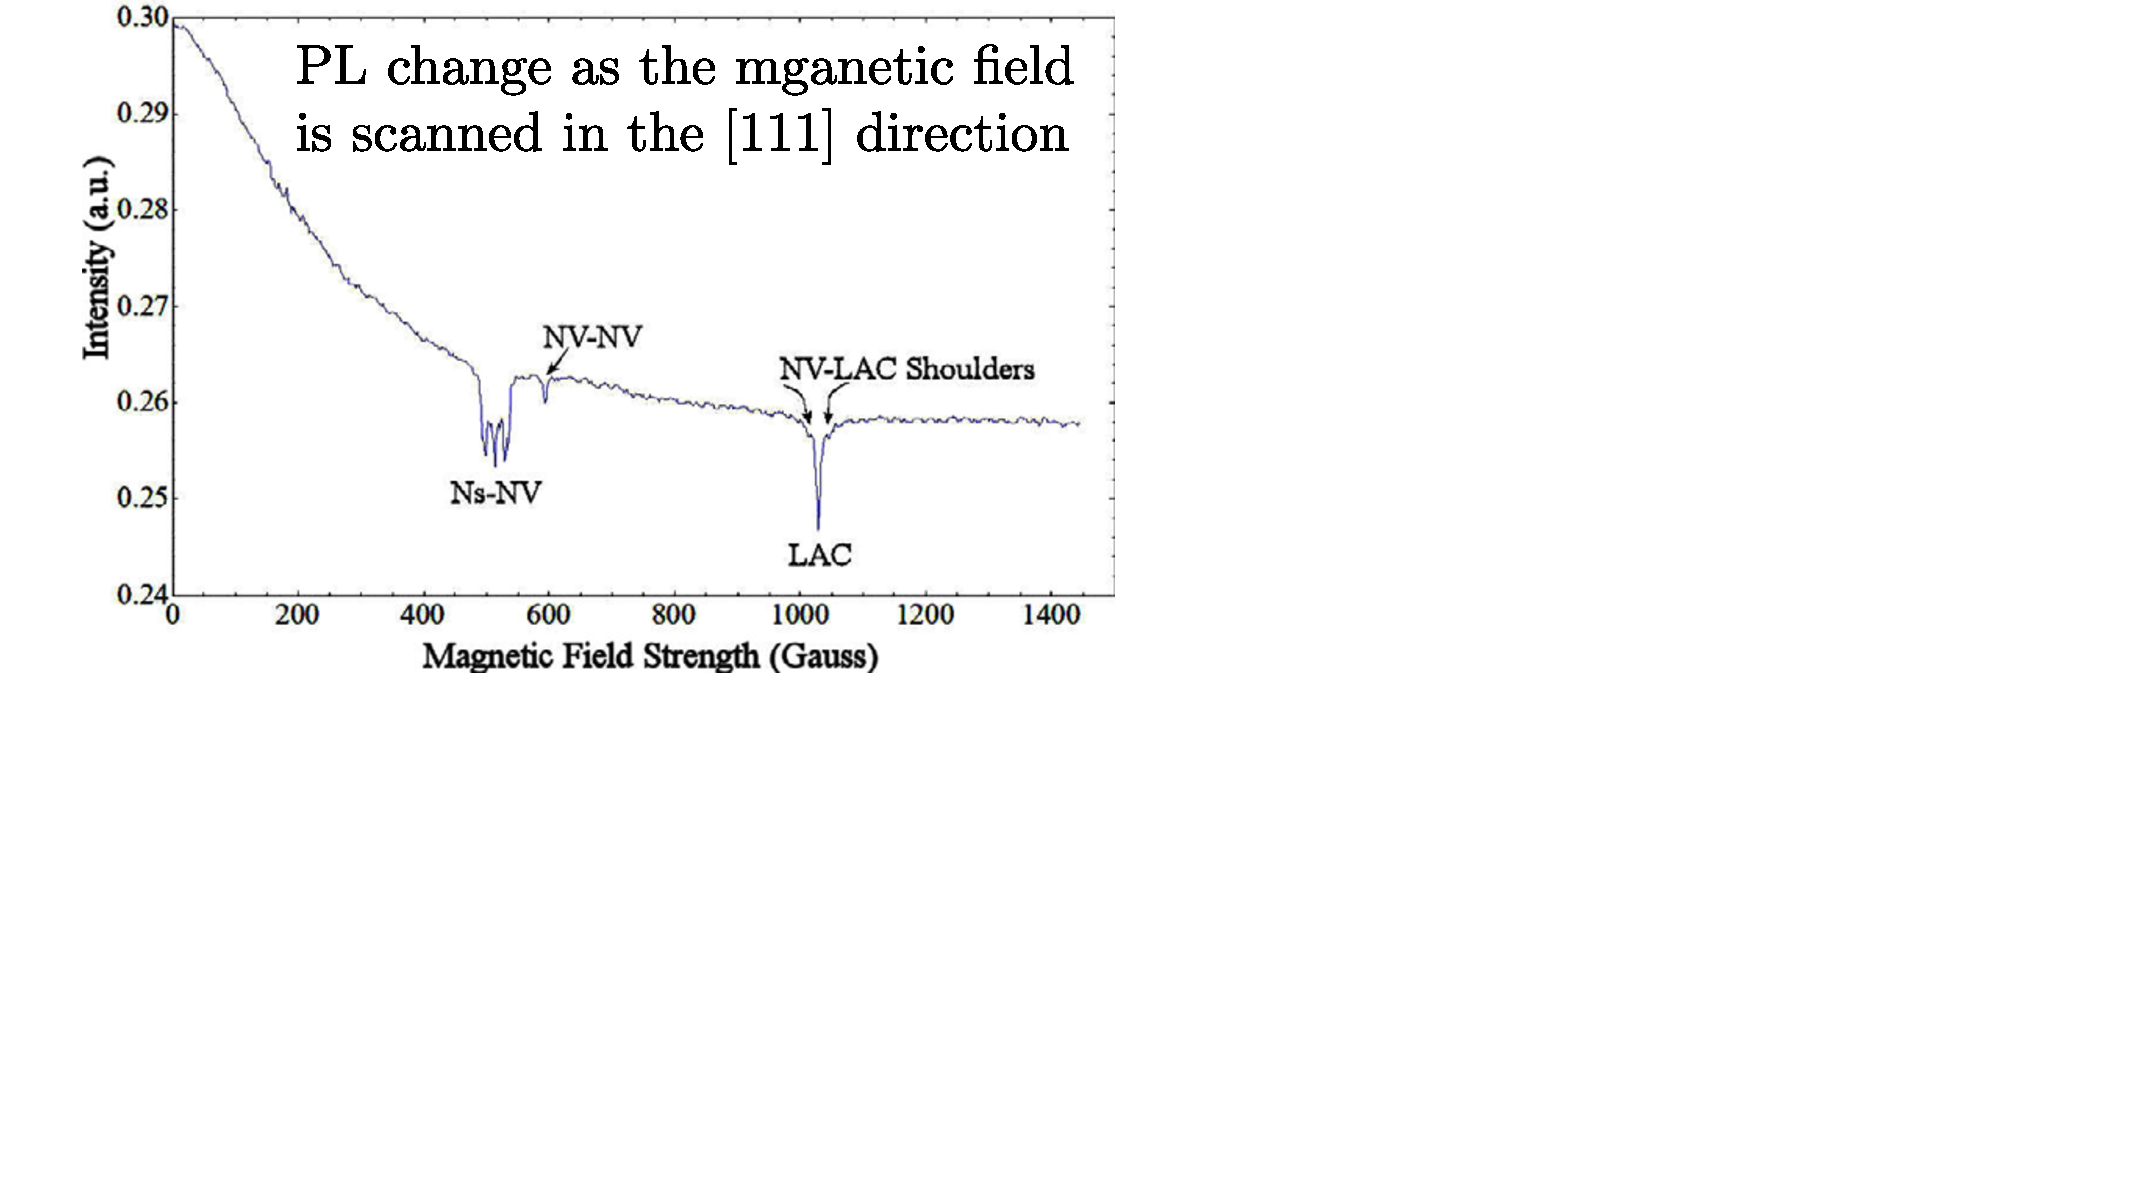
\includegraphics[scale=.30]{CR_111_0}\footfullcite{armstrong_nvnv_2010}
    \onslide<2>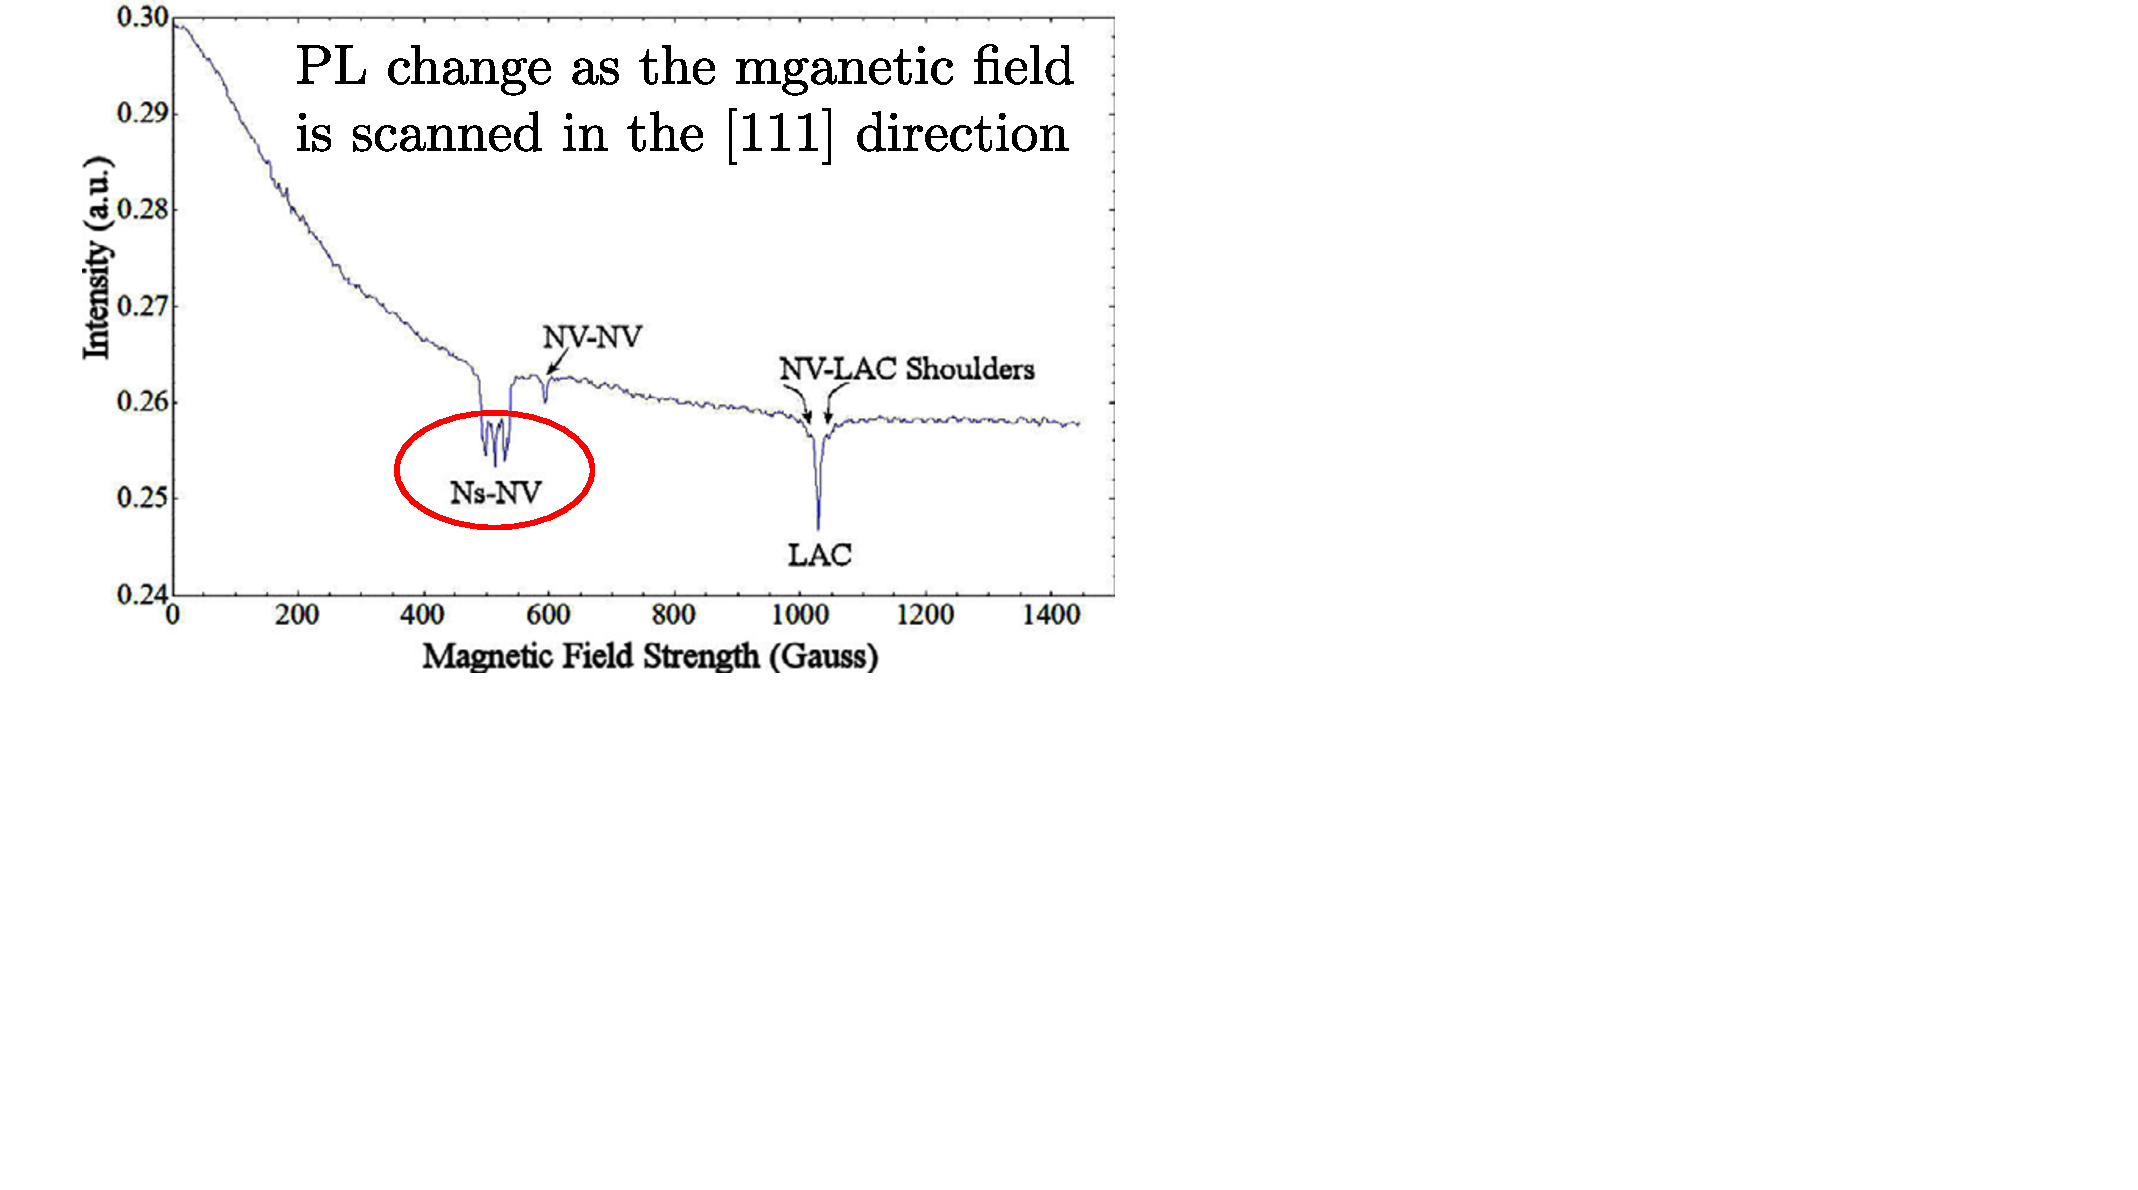
\includegraphics[scale=.30]{CR_111_05}
    \onslide<3>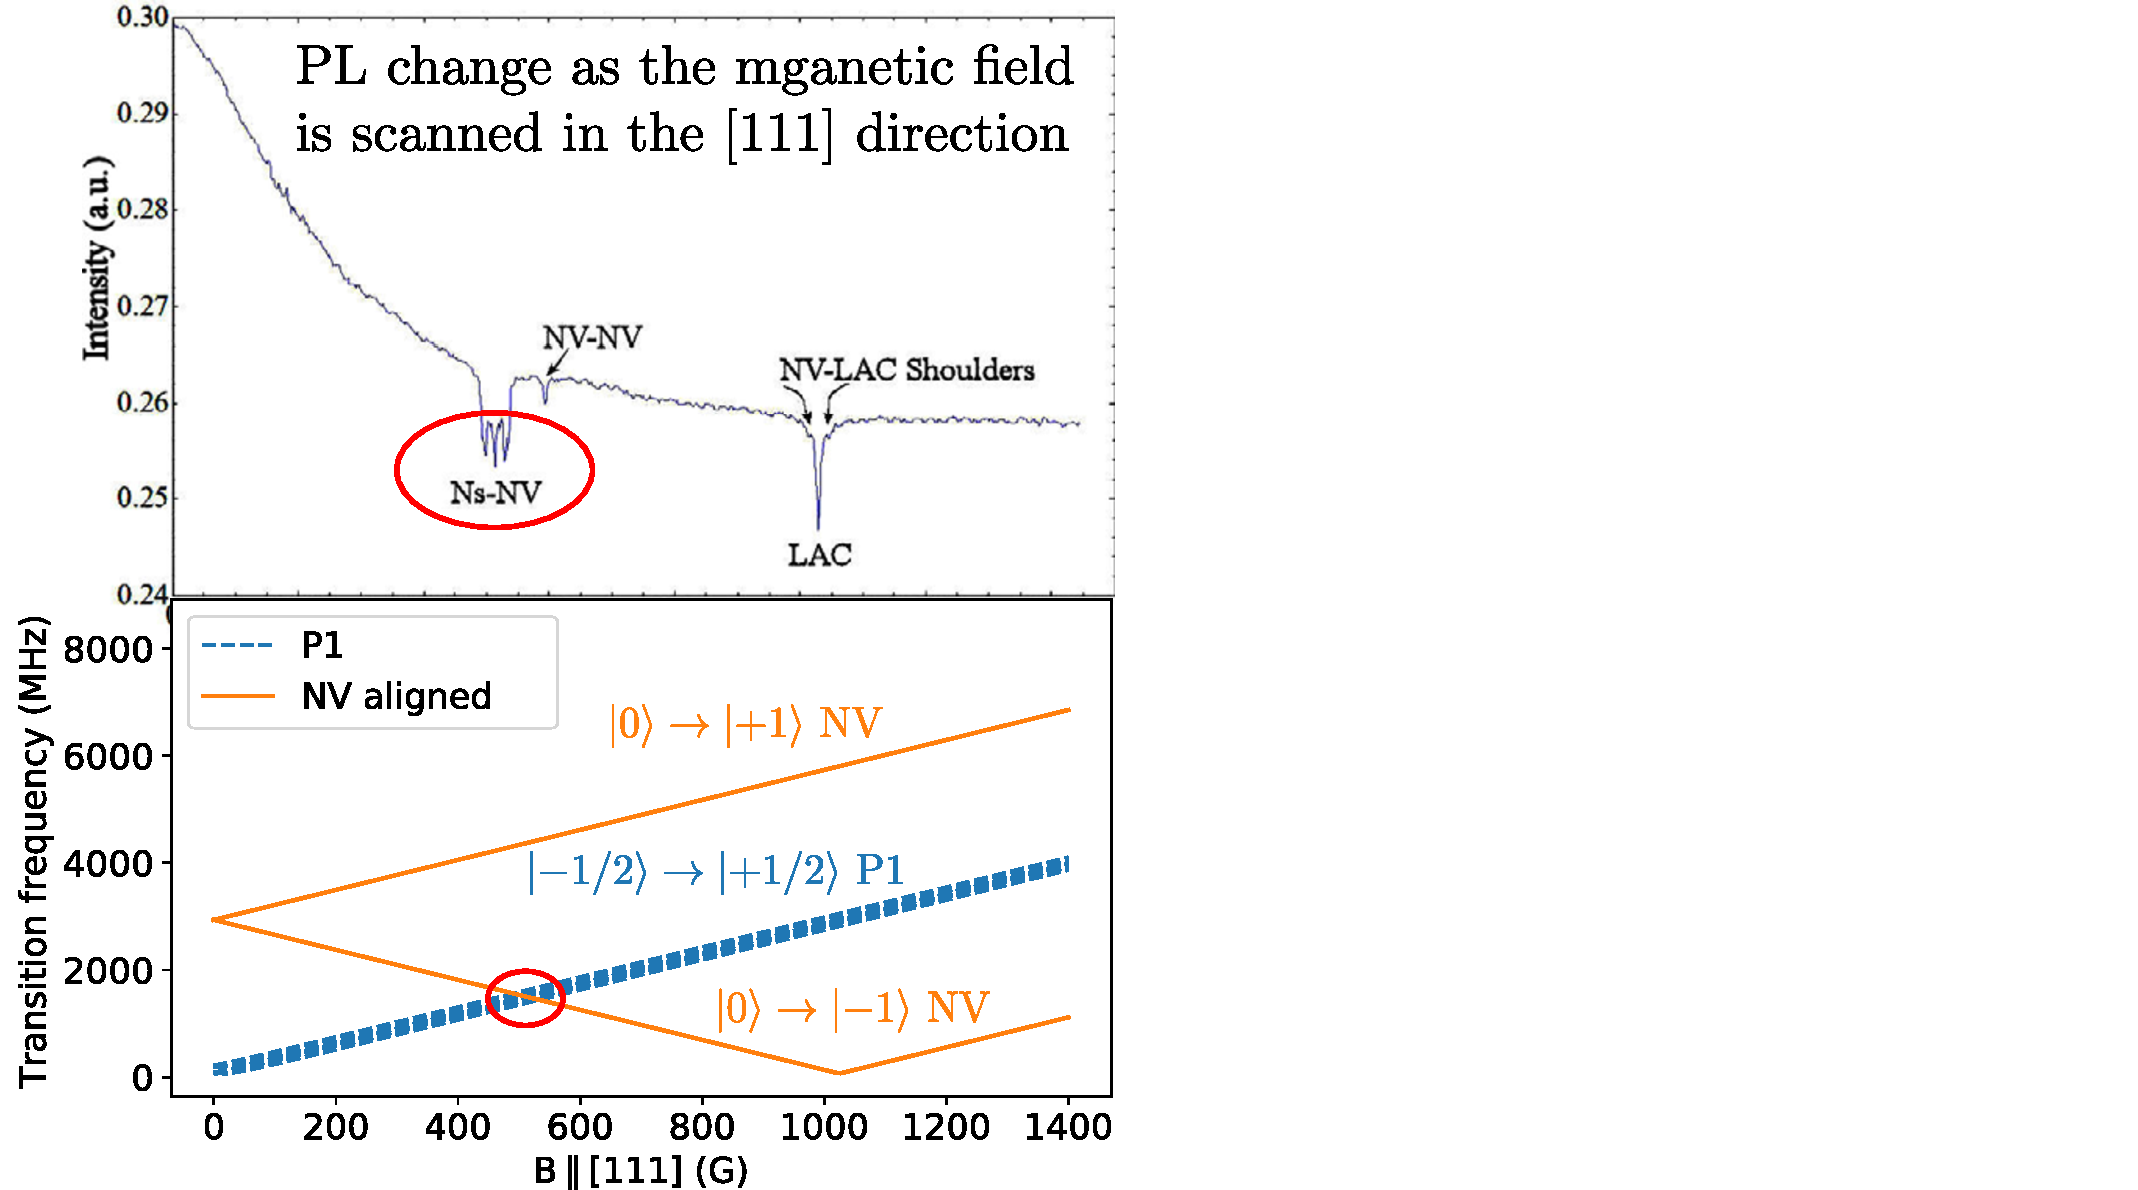
\includegraphics[scale=.30]{CR_111_1}
    \onslide<4>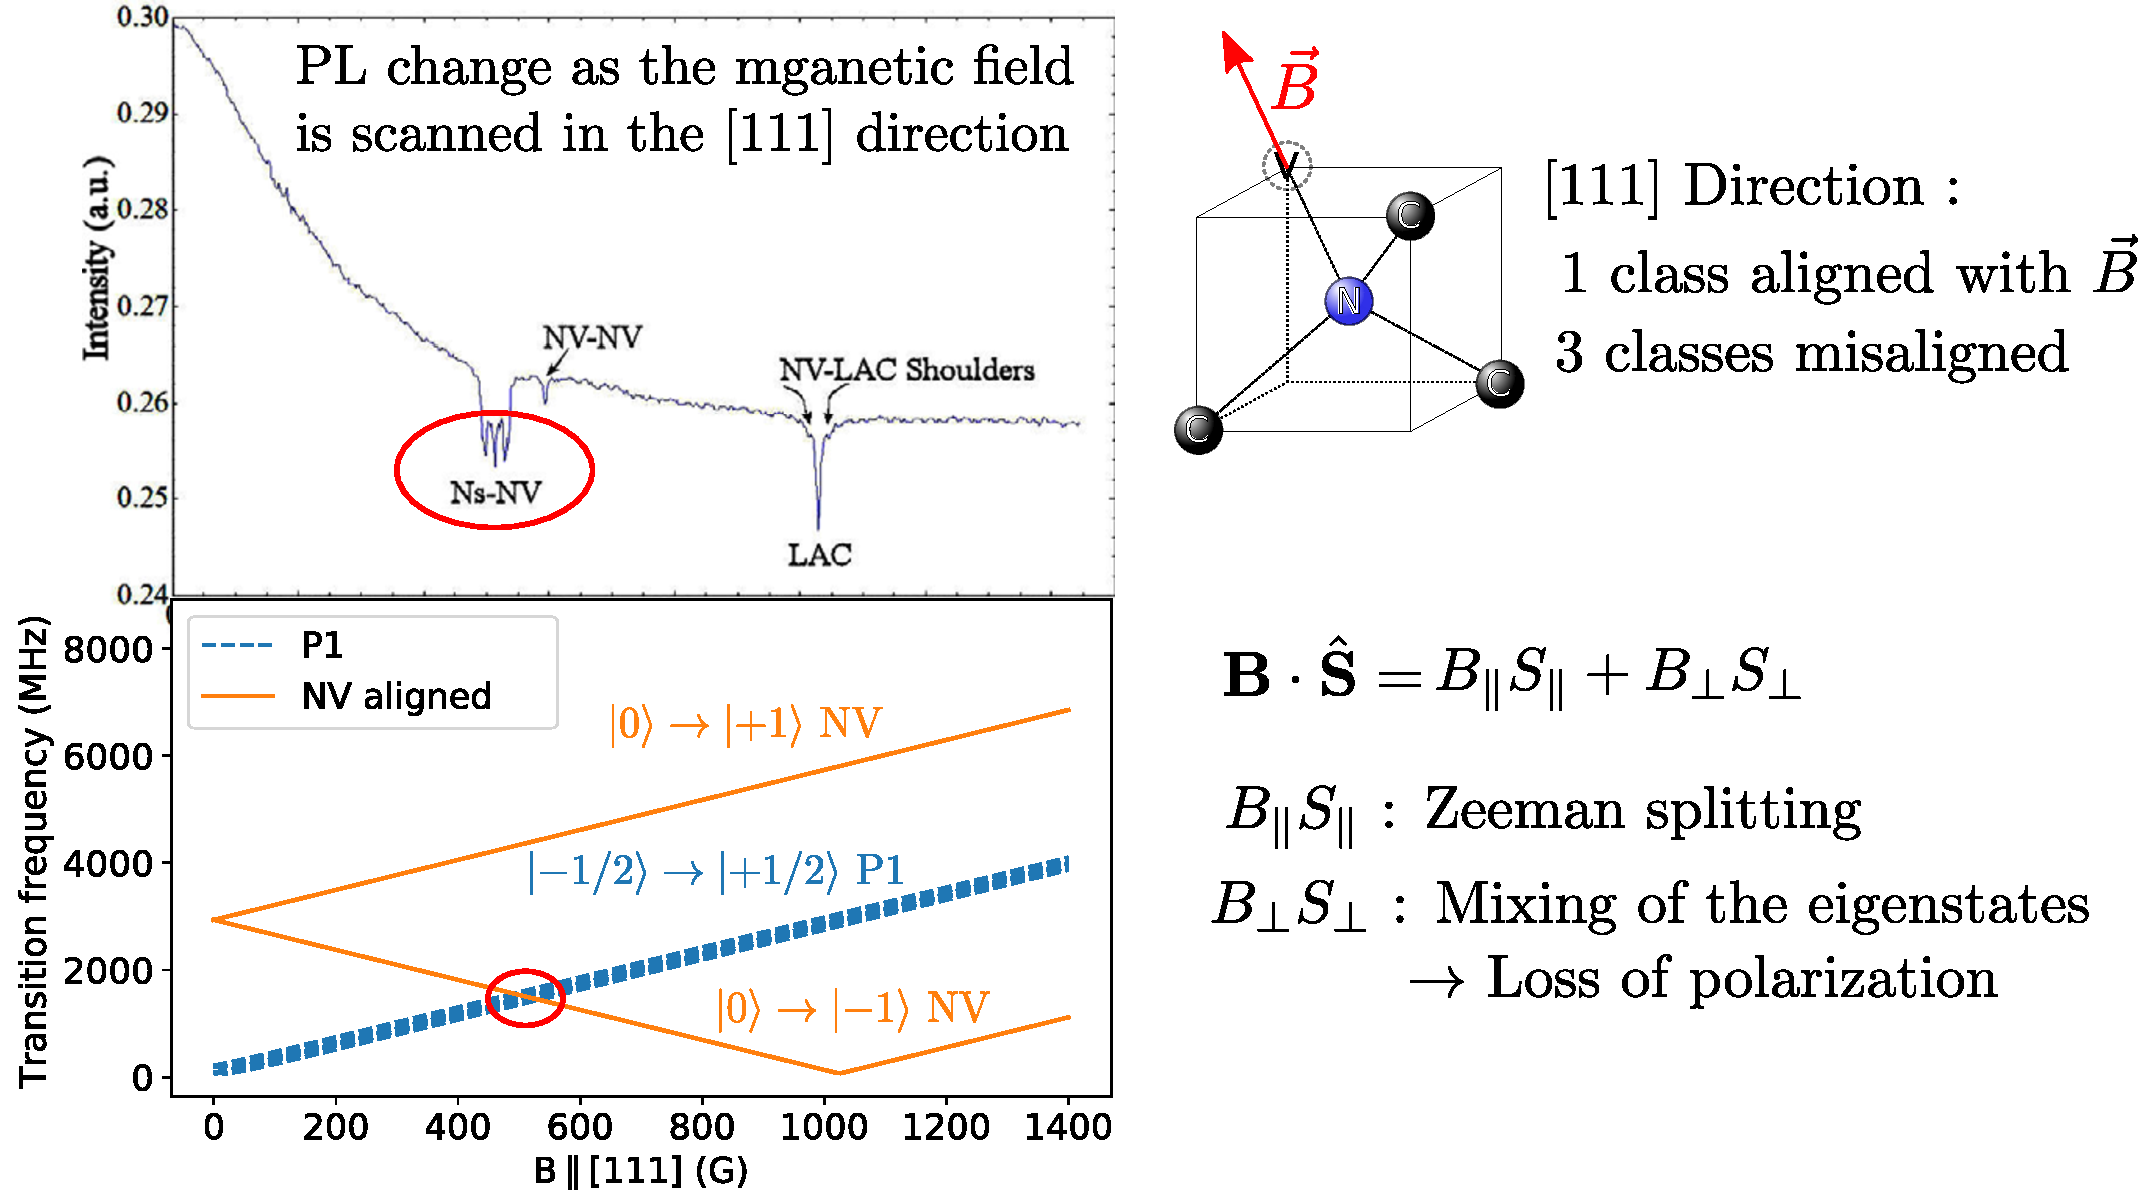
\includegraphics[scale=.30]{CR_111_2}
    \end{overprint}
\end{figure}
\end{frame}
\section{Cross-relaxations with new spin species}
\begin{frame}{Outline}
\tableofcontents[currentsection]
\end{frame}
\begin{frame}{Motivations of the study}
\begin{figure}
    \begin{overprint}
    \onslide<1>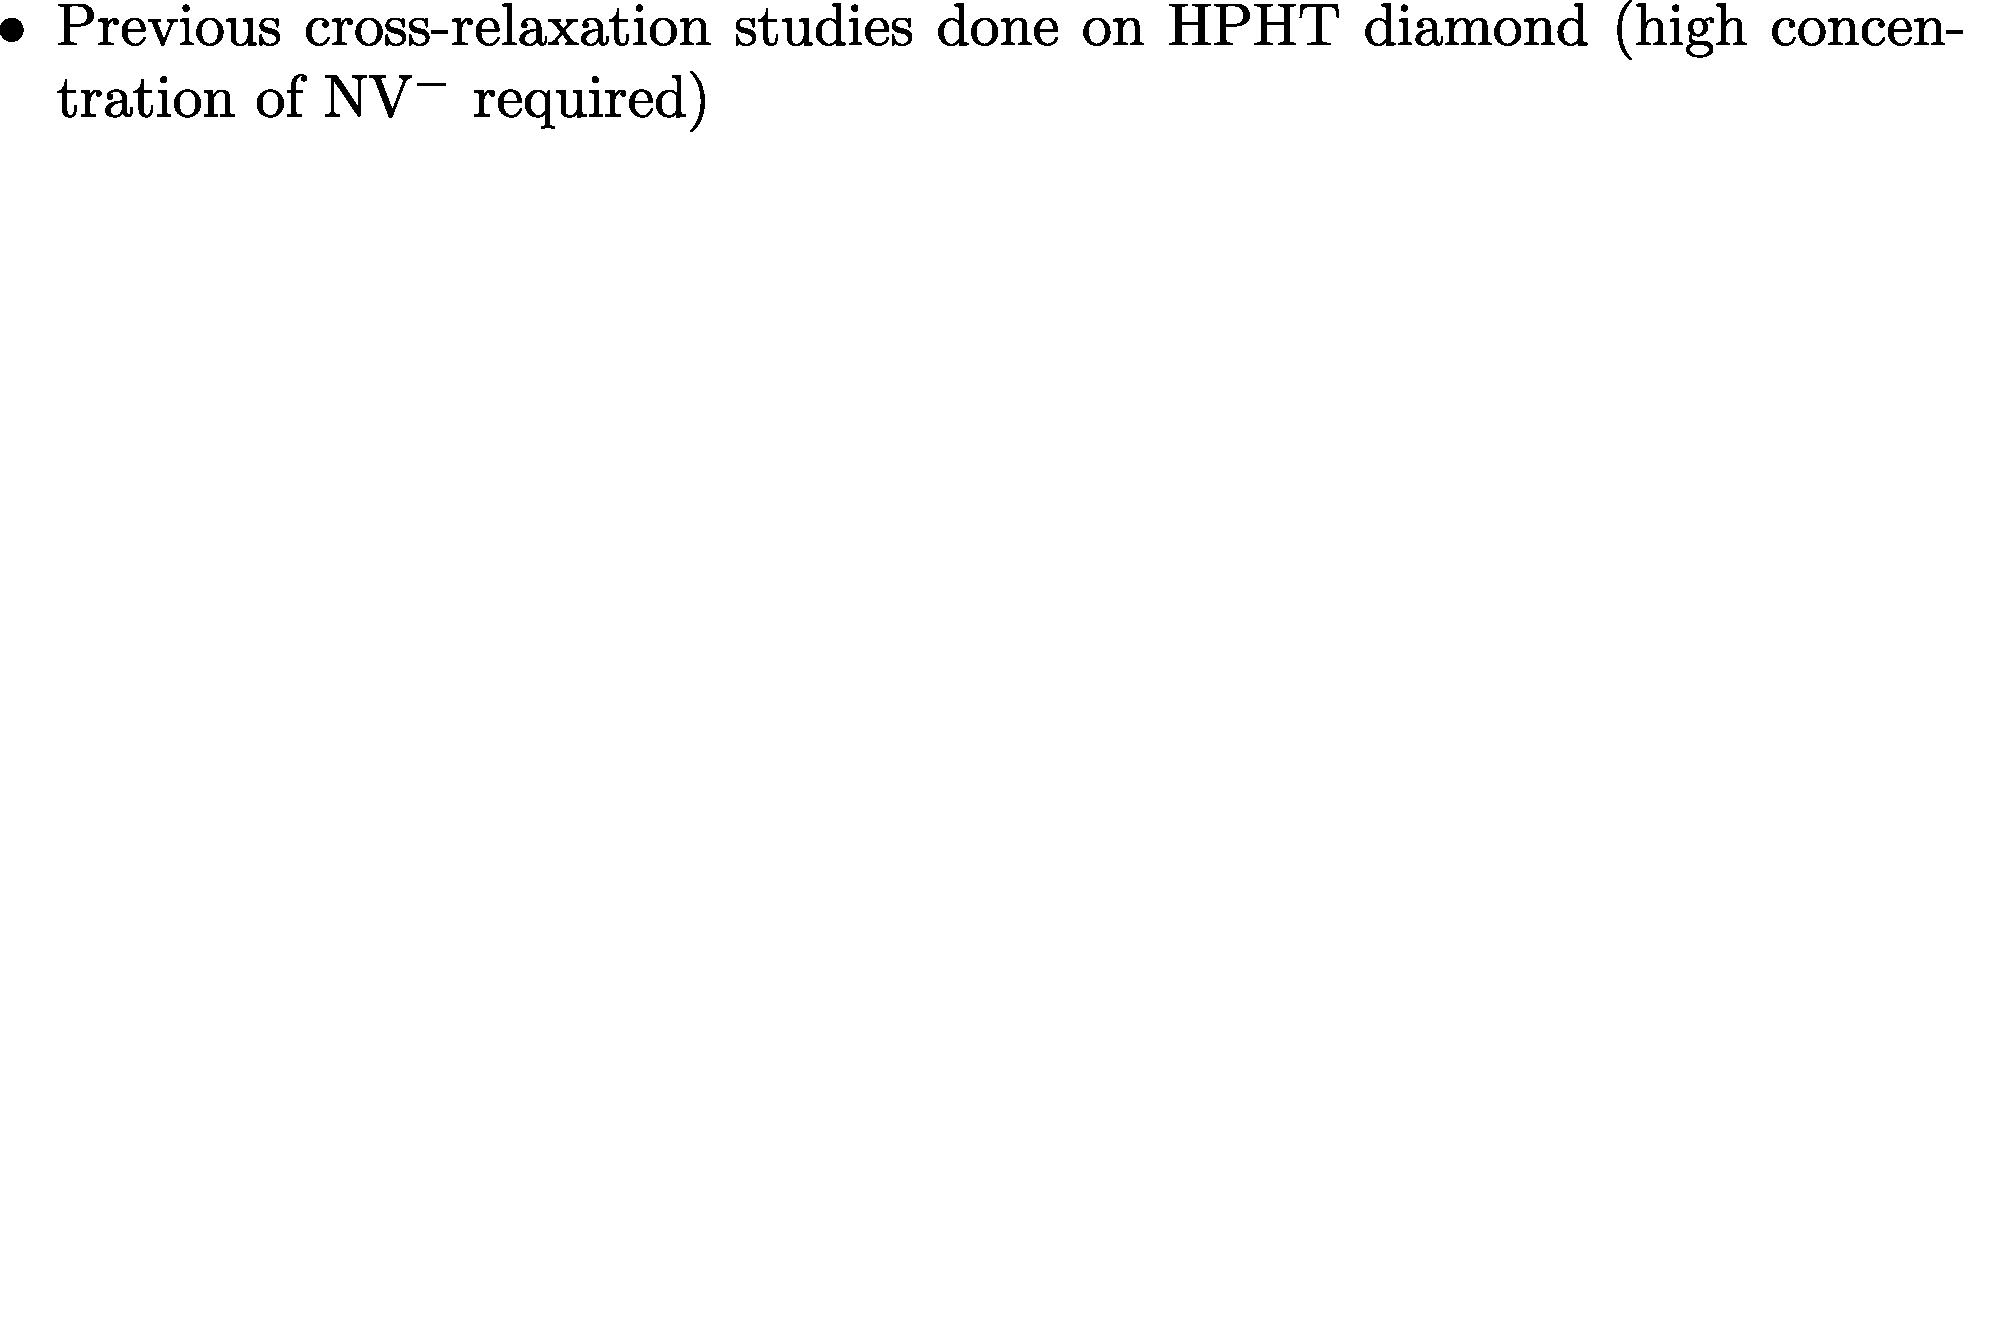
\includegraphics[scale=.30]{Motivations_0}
    \onslide<2>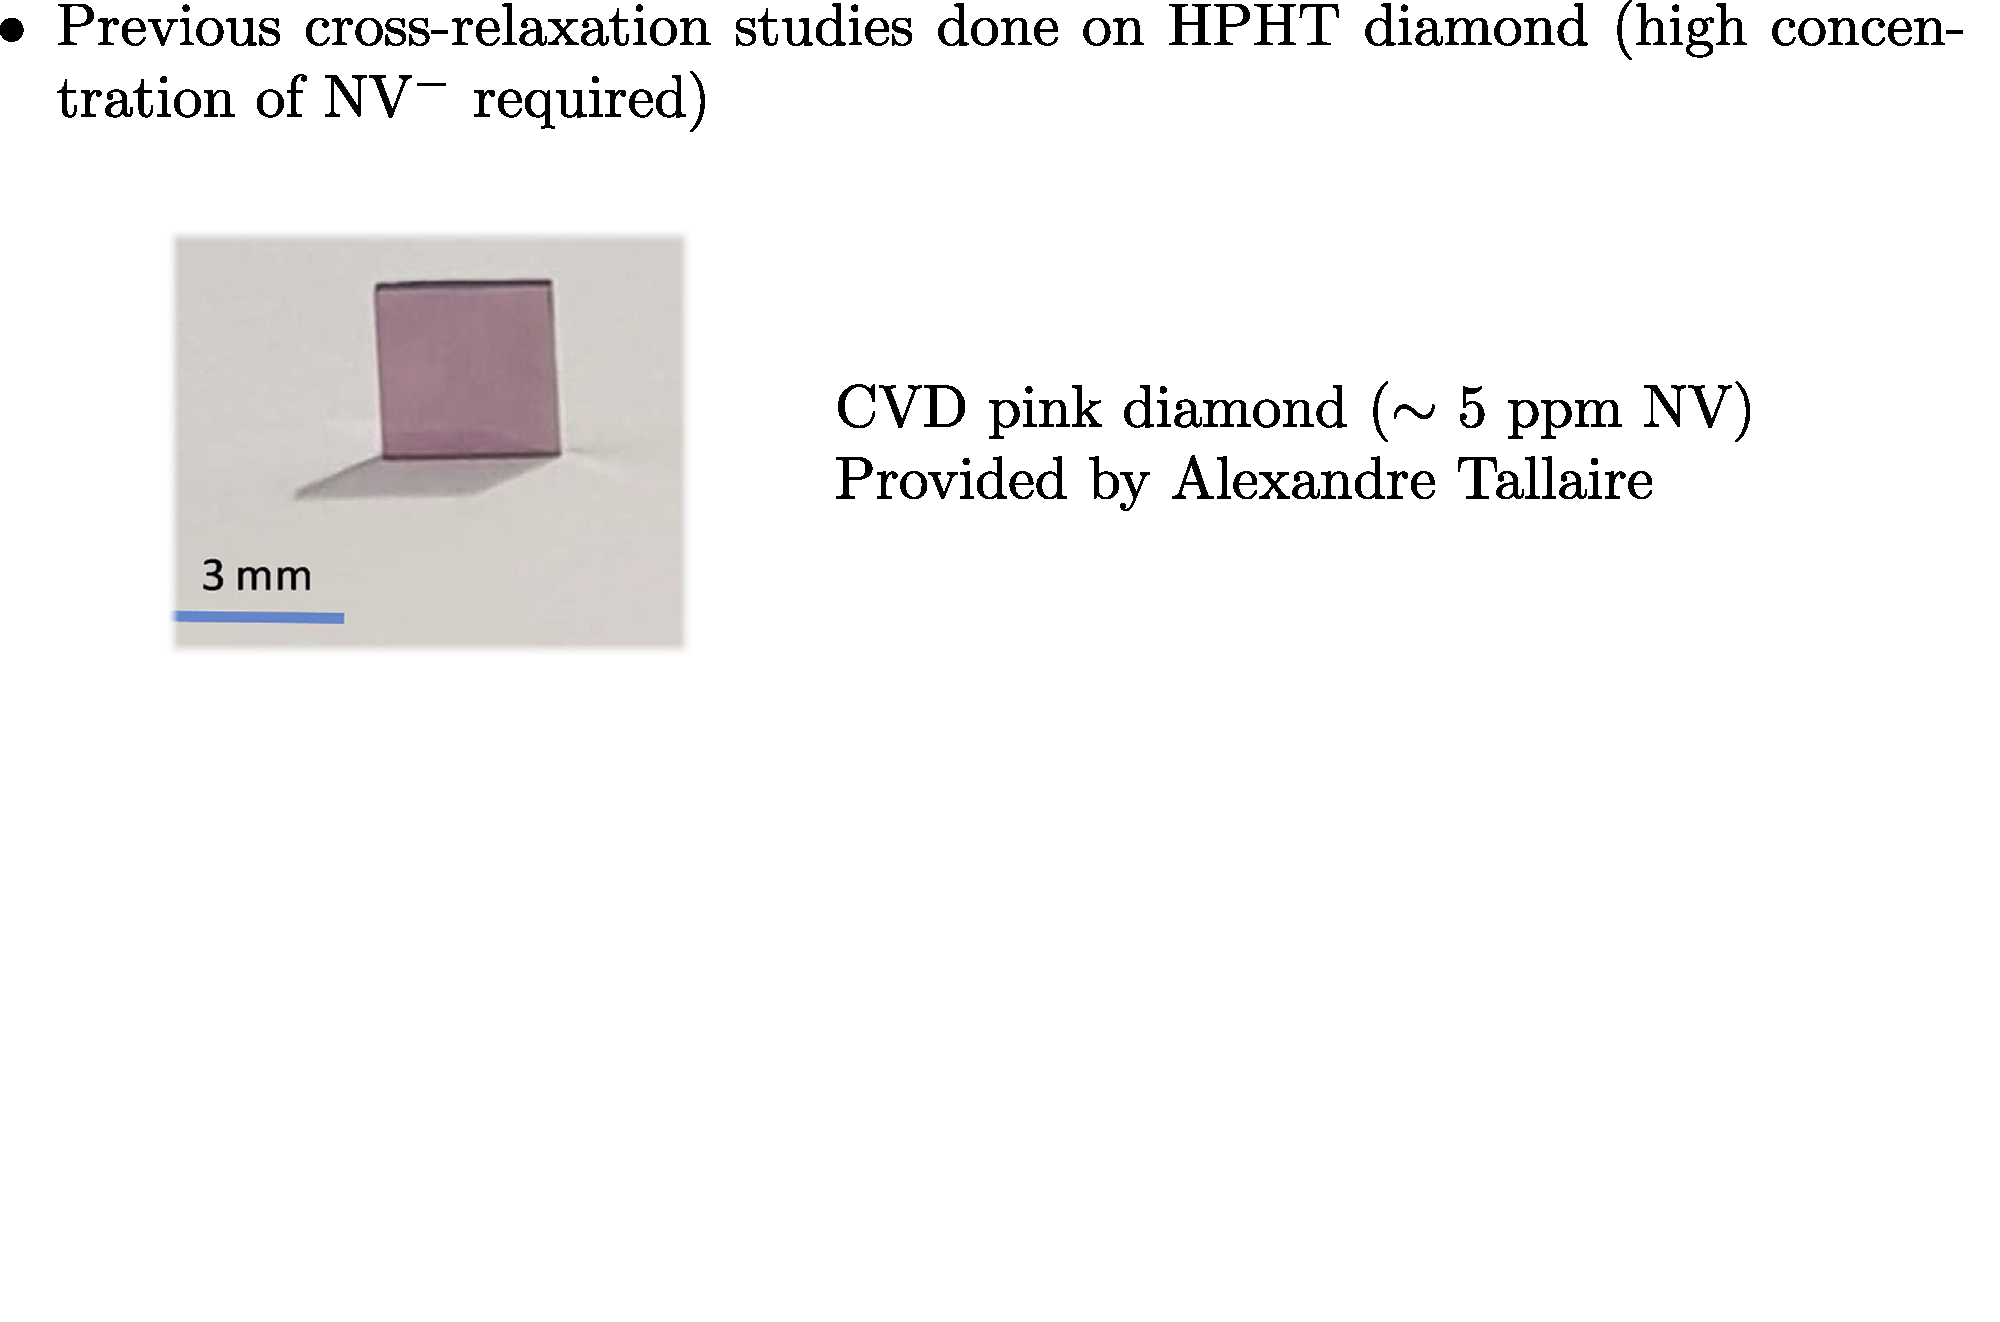
\includegraphics[scale=.30]{Motivations_1}\footfullcite{tallaire2020high}
    \onslide<3>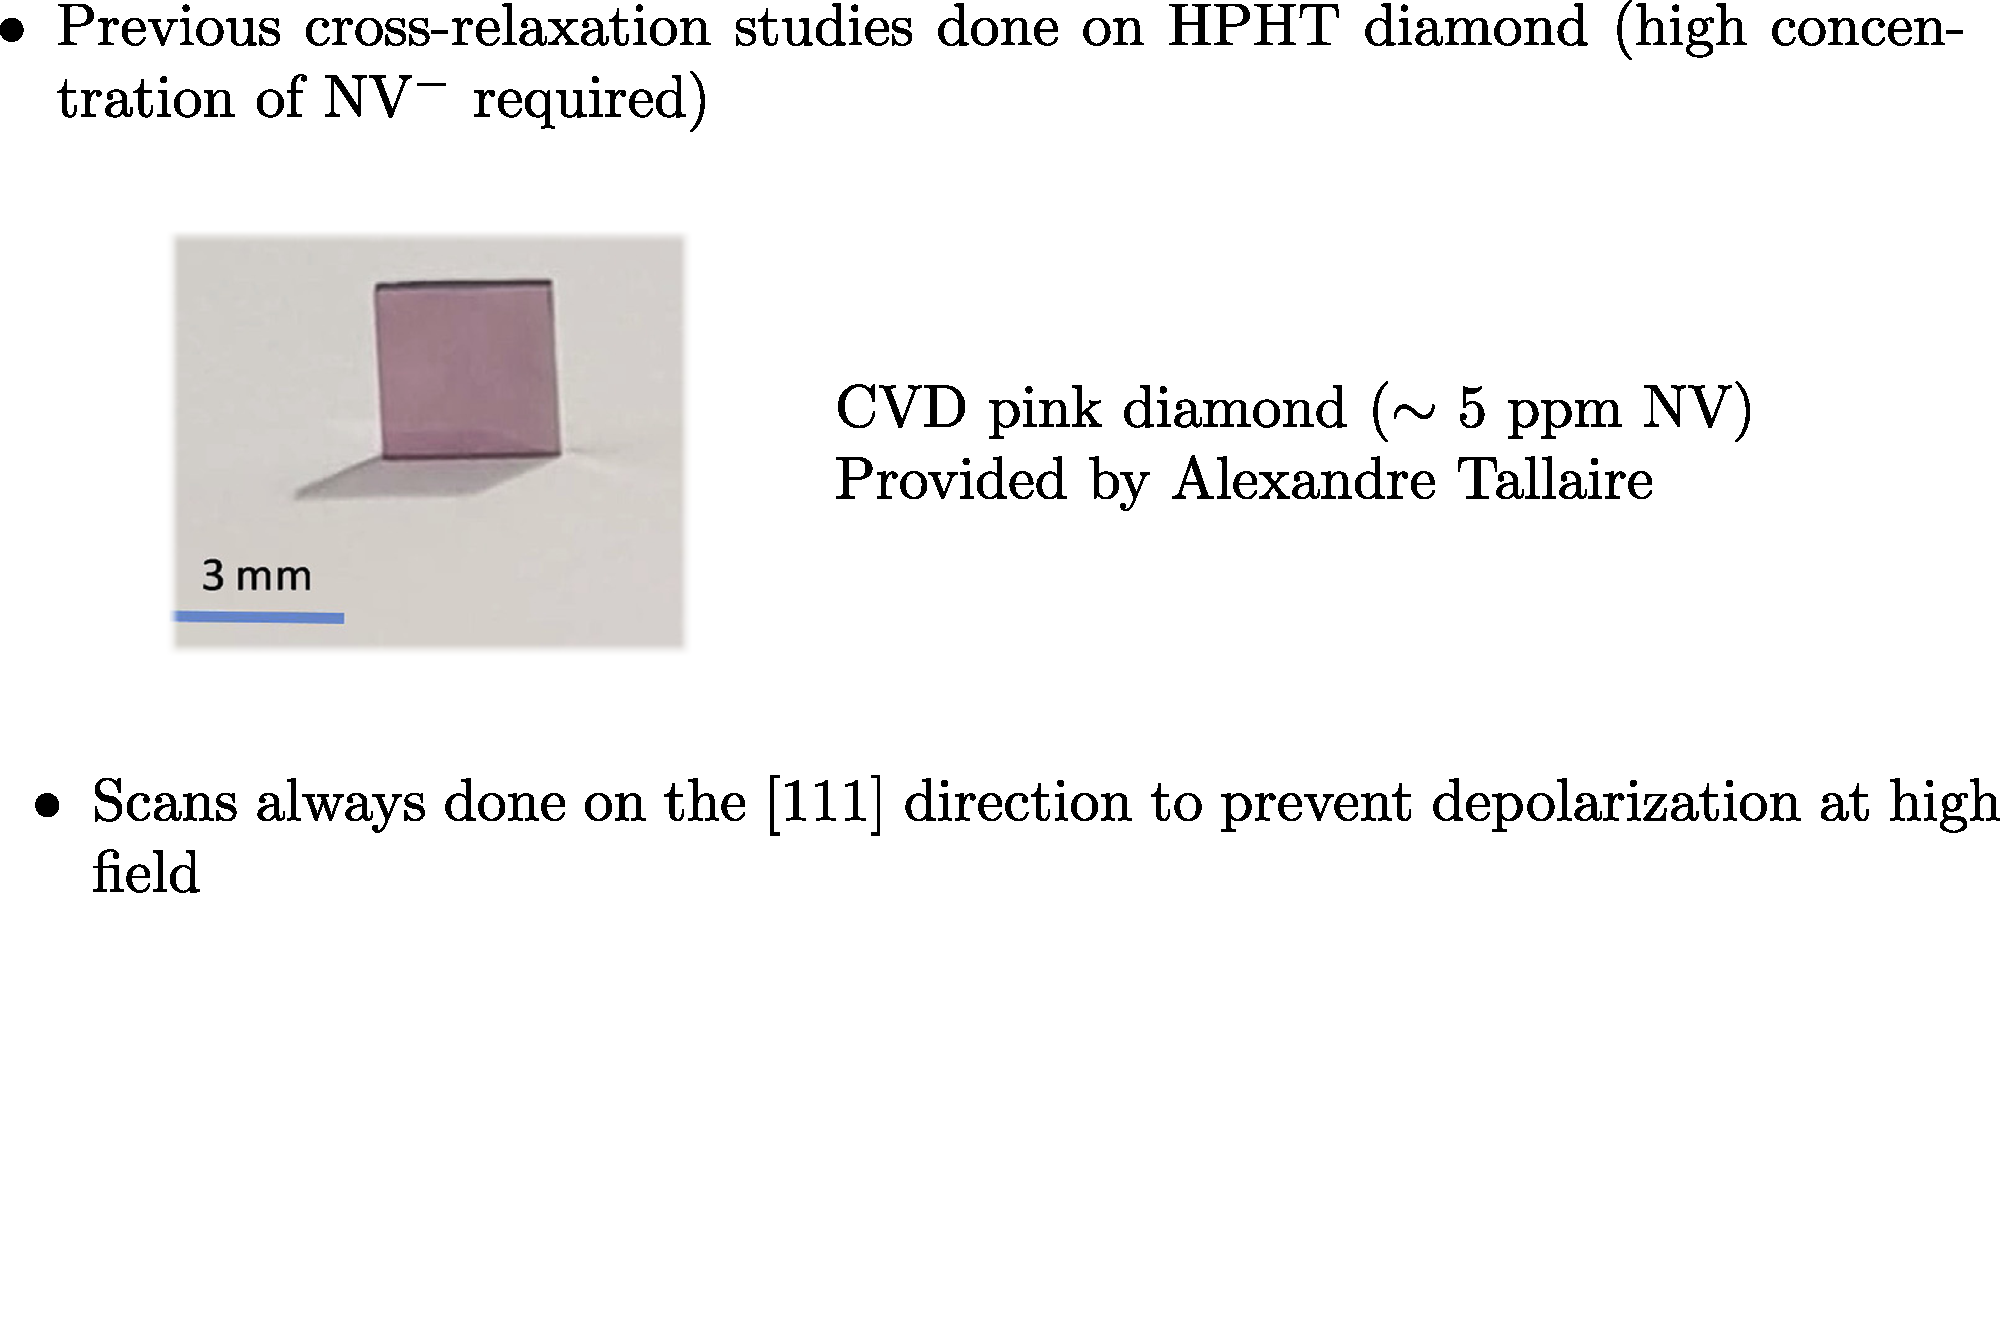
\includegraphics[scale=.30]{Motivations_2}
    \onslide<4>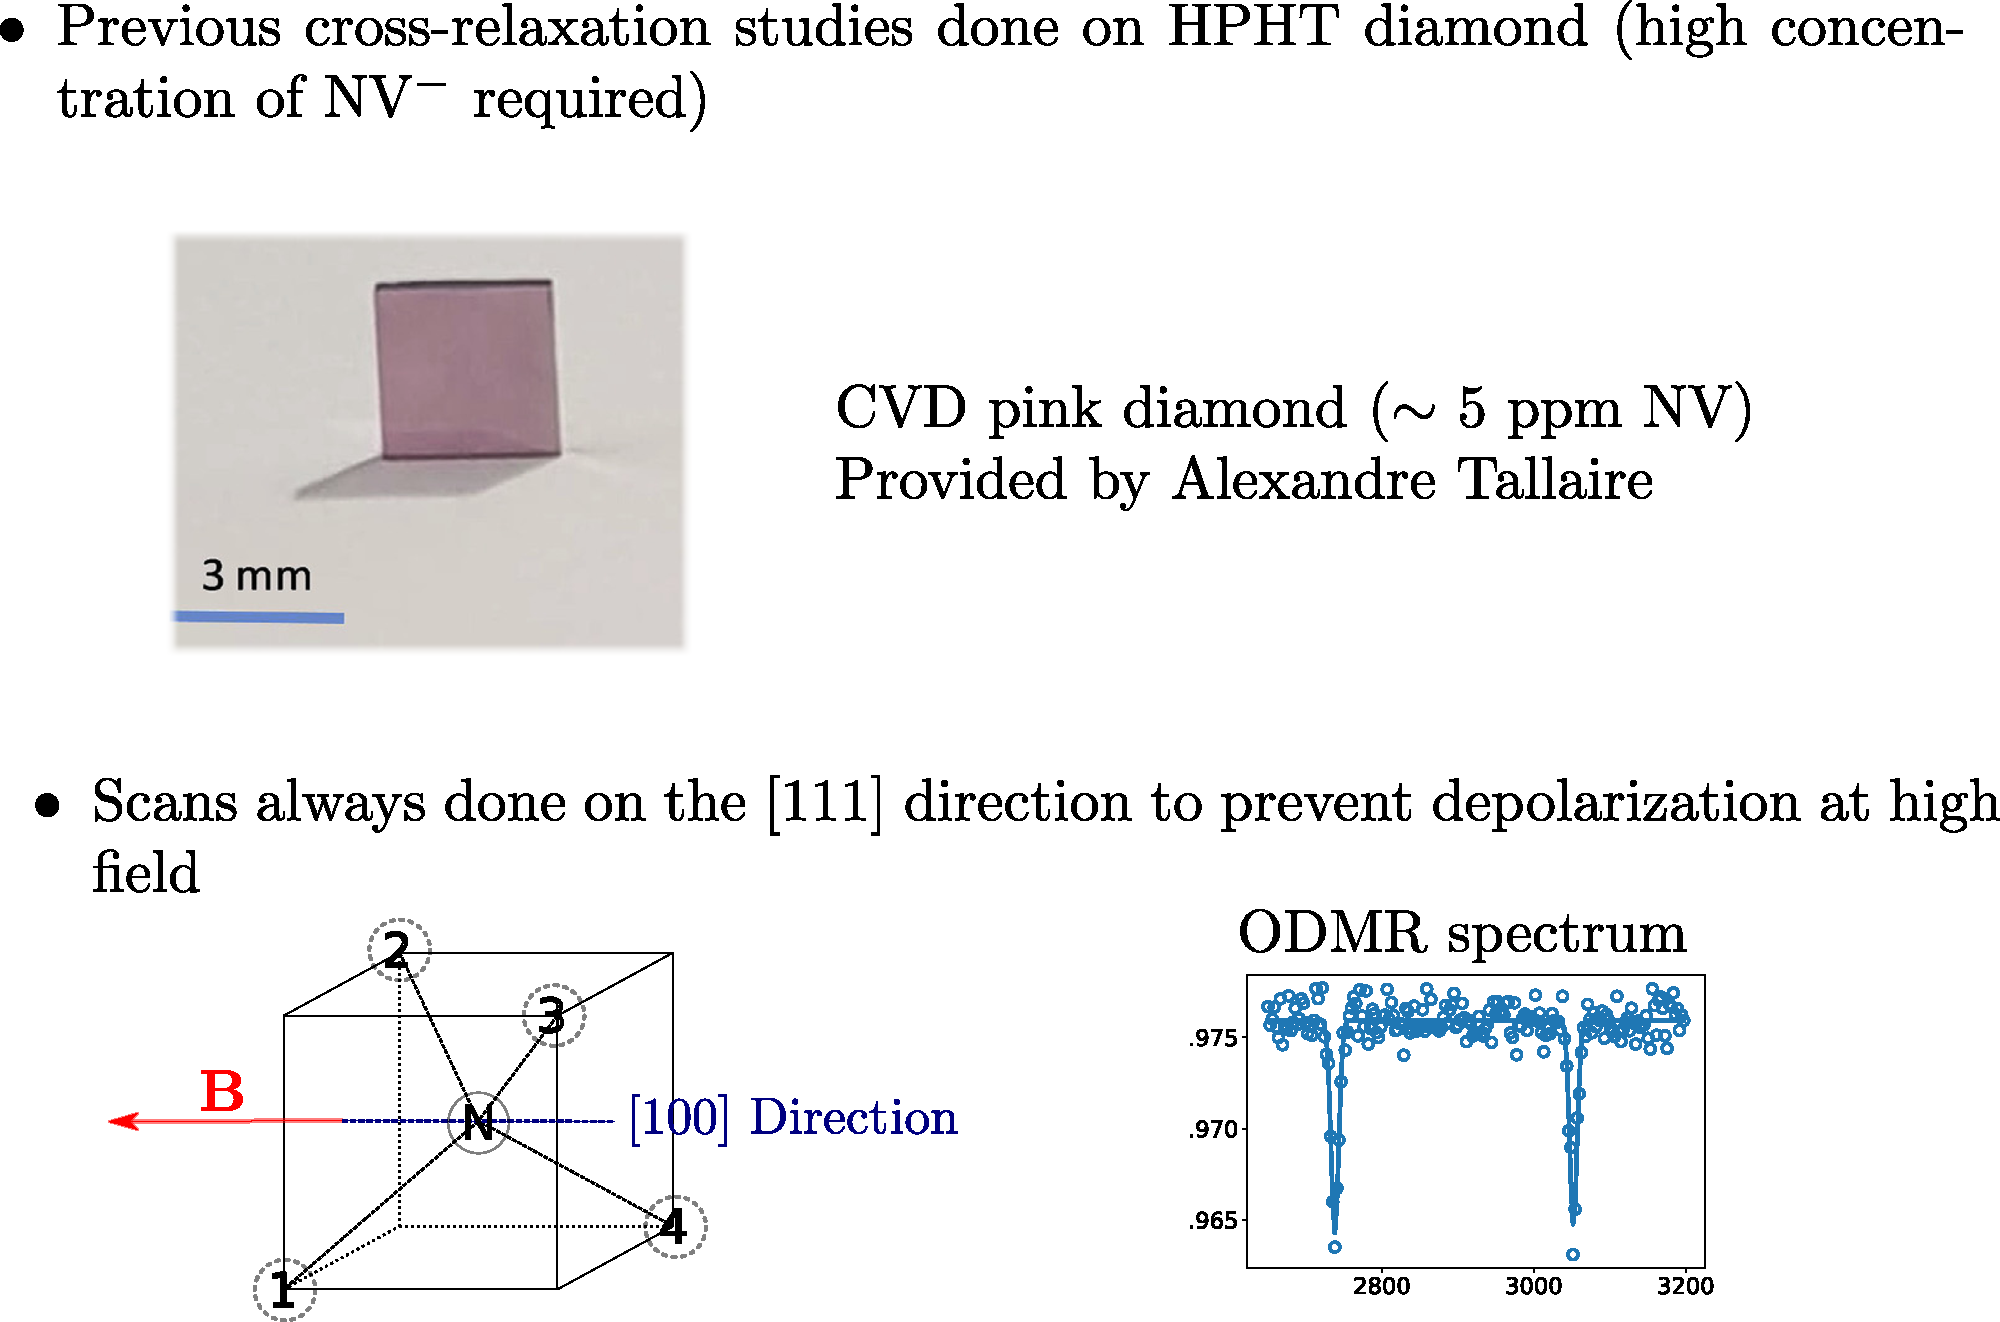
\includegraphics[scale=.30]{Motivations_3}
    \end{overprint}
\end{figure}
\end{frame}
\begin{frame}{Photoluminescence change with $\vec B$ in the [100] direction}
\begin{figure}
    \begin{overprint}
    \onslide<1>\centering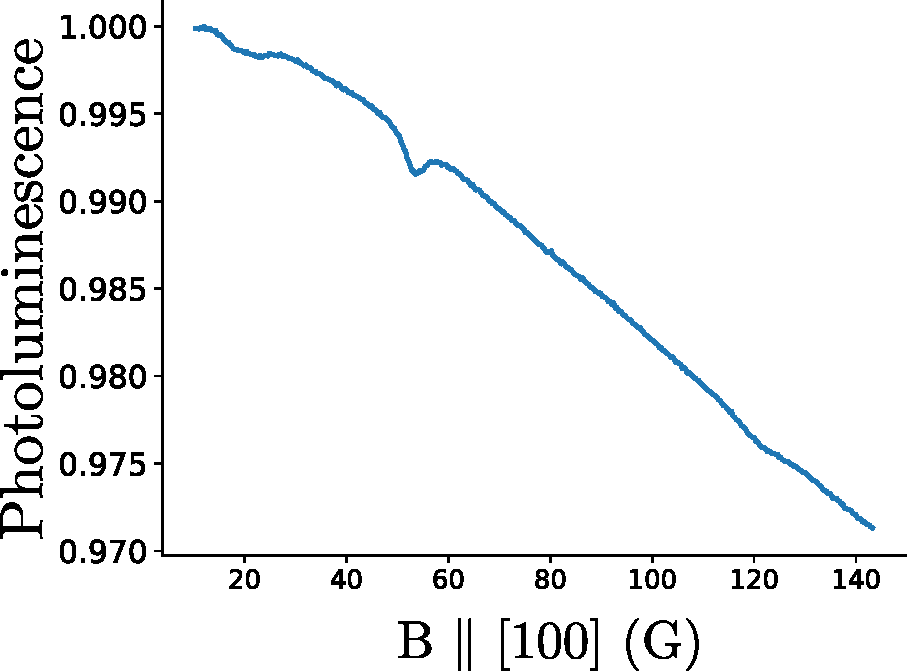
\includegraphics[scale=.45]{Scan_100_brut_0}
    \onslide<2>\centering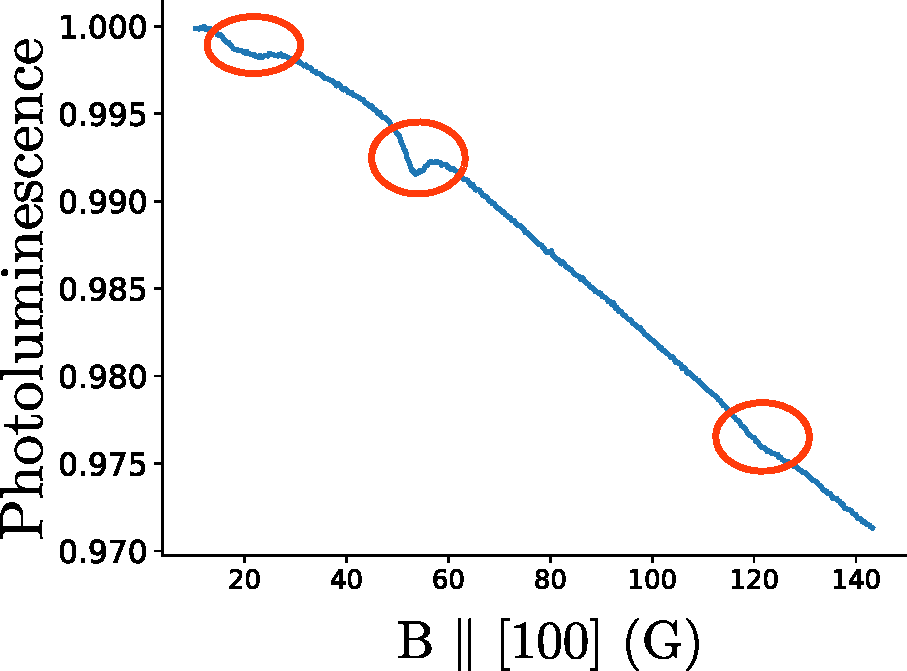
\includegraphics[scale=.45]{Scan_100_brut_1}
    \onslide<3>\centering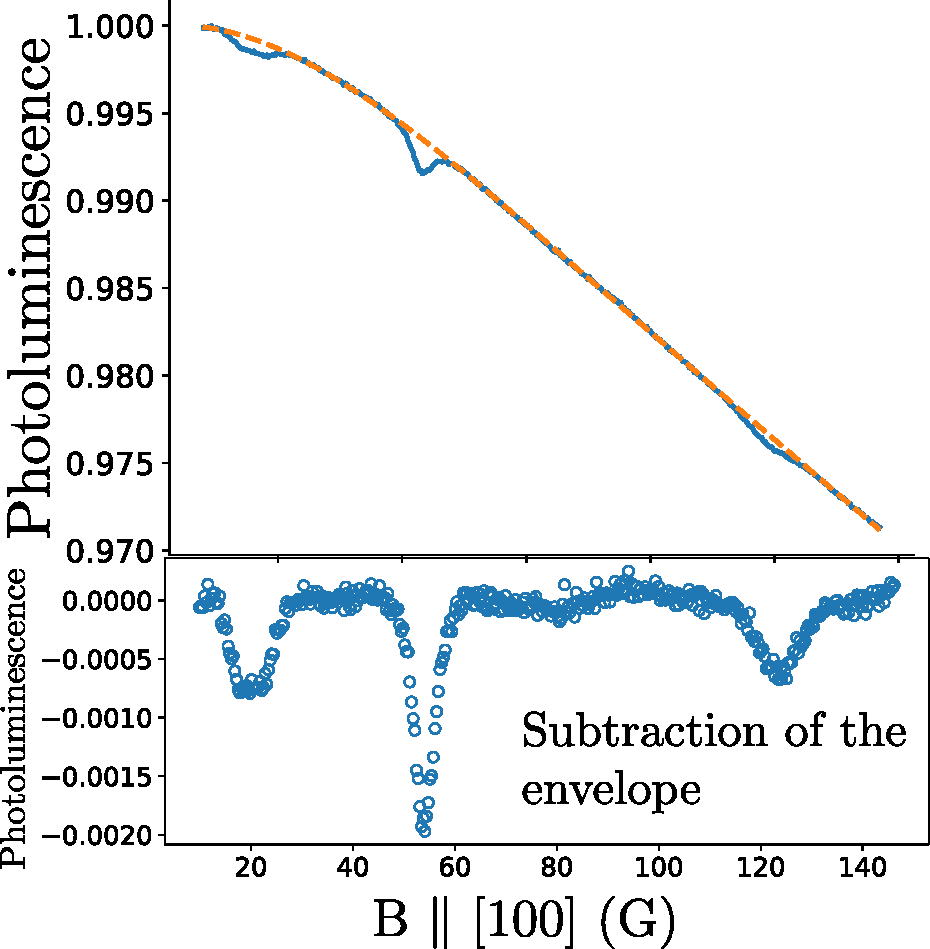
\includegraphics[scale=.45]{Scan_100_brut_2}
    \end{overprint}
\end{figure}
\end{frame}
\begin{frame}{Cross-relaxation between NV$^-$ and VH$^-$}
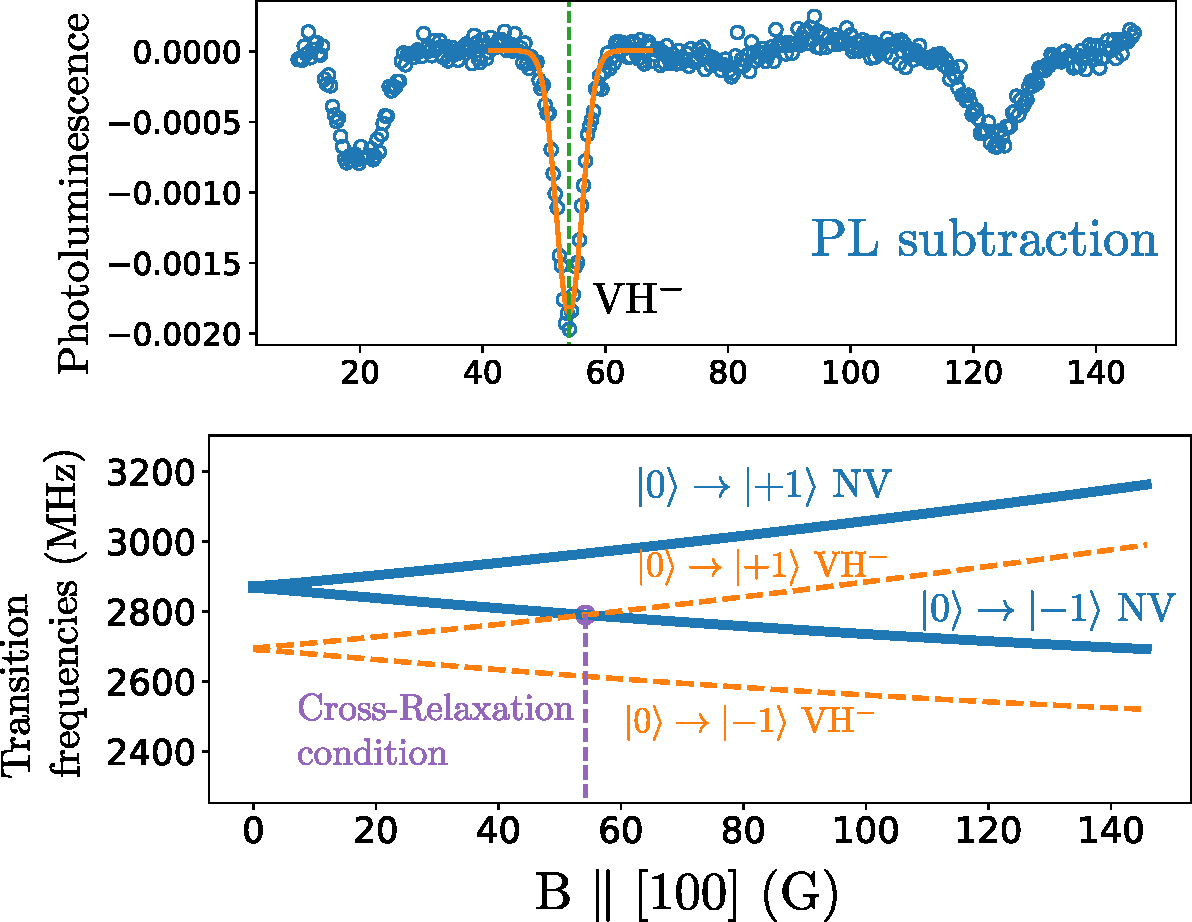
\includegraphics[scale=.48]{soustraction_1}
\end{frame}
\begin{frame}{Cross-relaxation between NV$^-$ and WAR1}
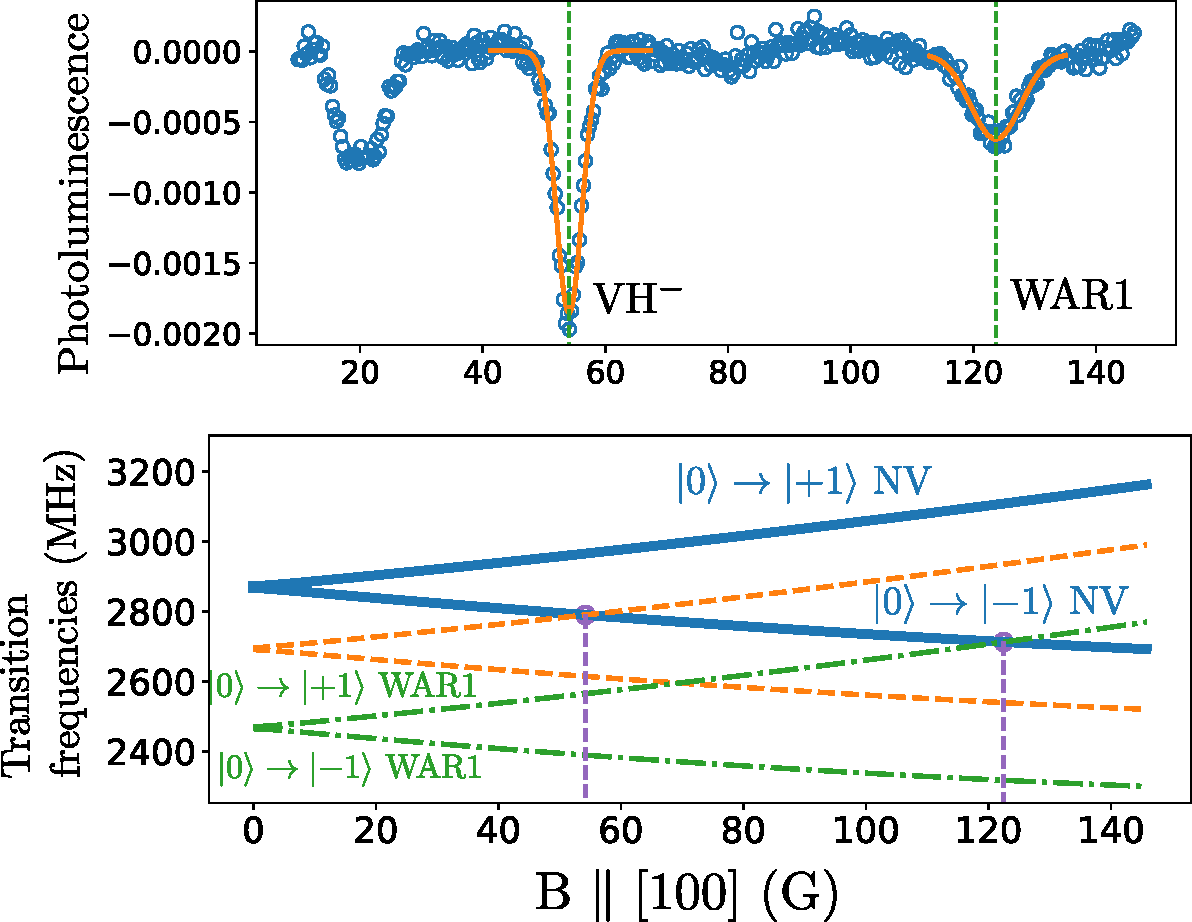
\includegraphics[scale=.48]{soustraction_2}
\end{frame}
\begin{frame}{EPR spectroscopy}
Electron Paramagnetic Resonance : A spectroscopy technique using absorption of a microwave at a given frequency (9.5 GHz for example) as a function of magnetic field to detect paramagnetic defects.
\bigbreak
VH$^-$\footfullcite{glover_hydrogen_2004} and WAR1 \footfullcite{cruddace2007magnetic} have been observed by EPR spectrocopy in CVD diamonds by Mark Newton's team at the University of Warwick.
\end{frame}
\begin{frame}{Comparison between cross-relaxation and EPR}
\pause
Upsides :
\begin{itemize}
\item CR experiments are much simpler to setup (and less expensive!) : low $\vec B$, no microwave.
\end{itemize}
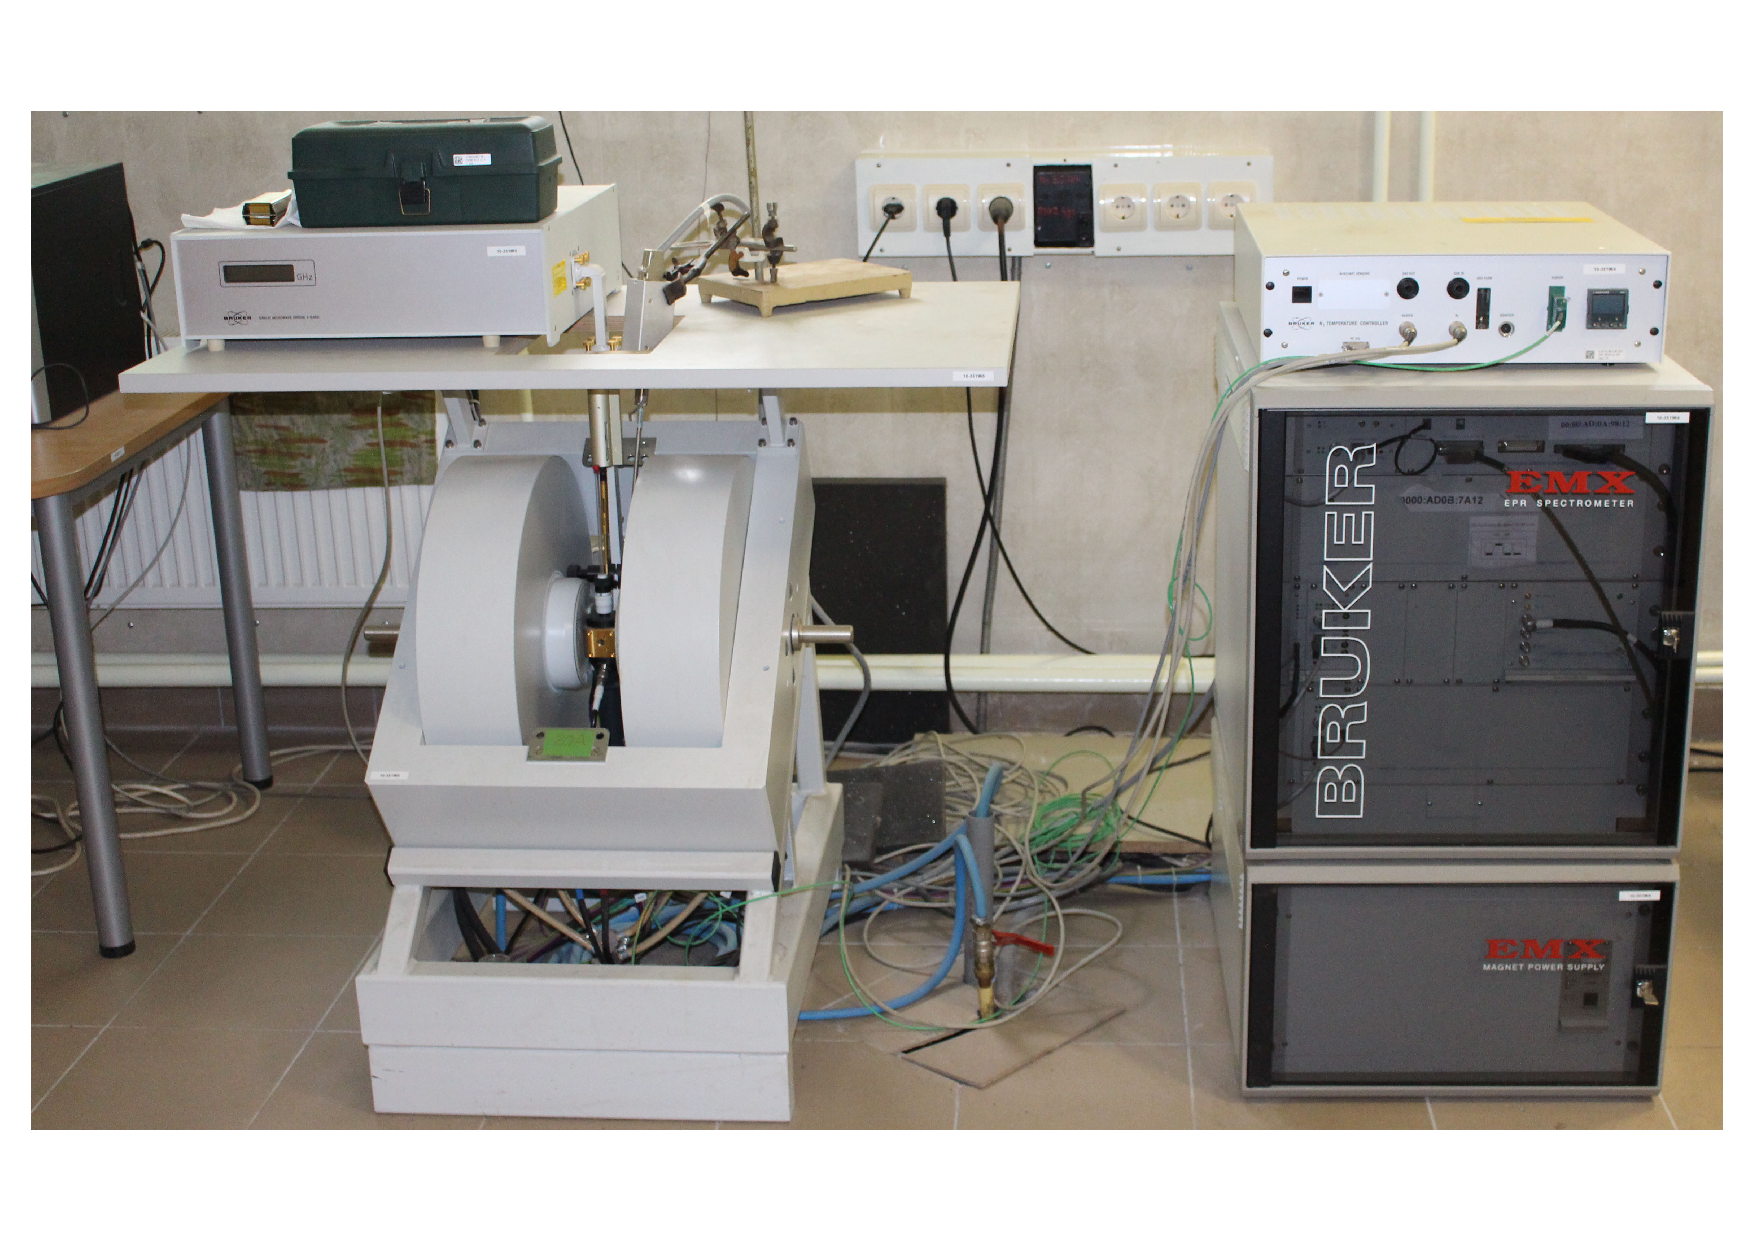
\includegraphics[scale=.3]{epr-converted}
\end{frame}
\begin{frame}{Comparison between cross-relaxation and EPR}
Upsides :
\begin{itemize}
\item CR experiments are much simpler to setup (and less expensive!) : low $\vec B$, no microwave.
\item Doable on micro and potentially nano-diamonds
\pause
\item NV centers produce a calibration for $\vec B$ $\to$ Better precision on the ZFS measurement
\pause
\item Potential for hyperpolarization of new spins
\pause
\end{itemize}
Downsides :
\begin{itemize}
\item Requires a high NV concentration
\pause
\item Loss of contrast in non-[100] directions
\end{itemize}
\end{frame}
\section{Cross-relaxation between NV centers}
\begin{frame}{Outline}
\tableofcontents[currentsection]
\end{frame}
\begin{frame}{Experimental proofs of NV-NV cross-relaxations}
\begin{figure}
    \begin{overprint}
    \onslide<1>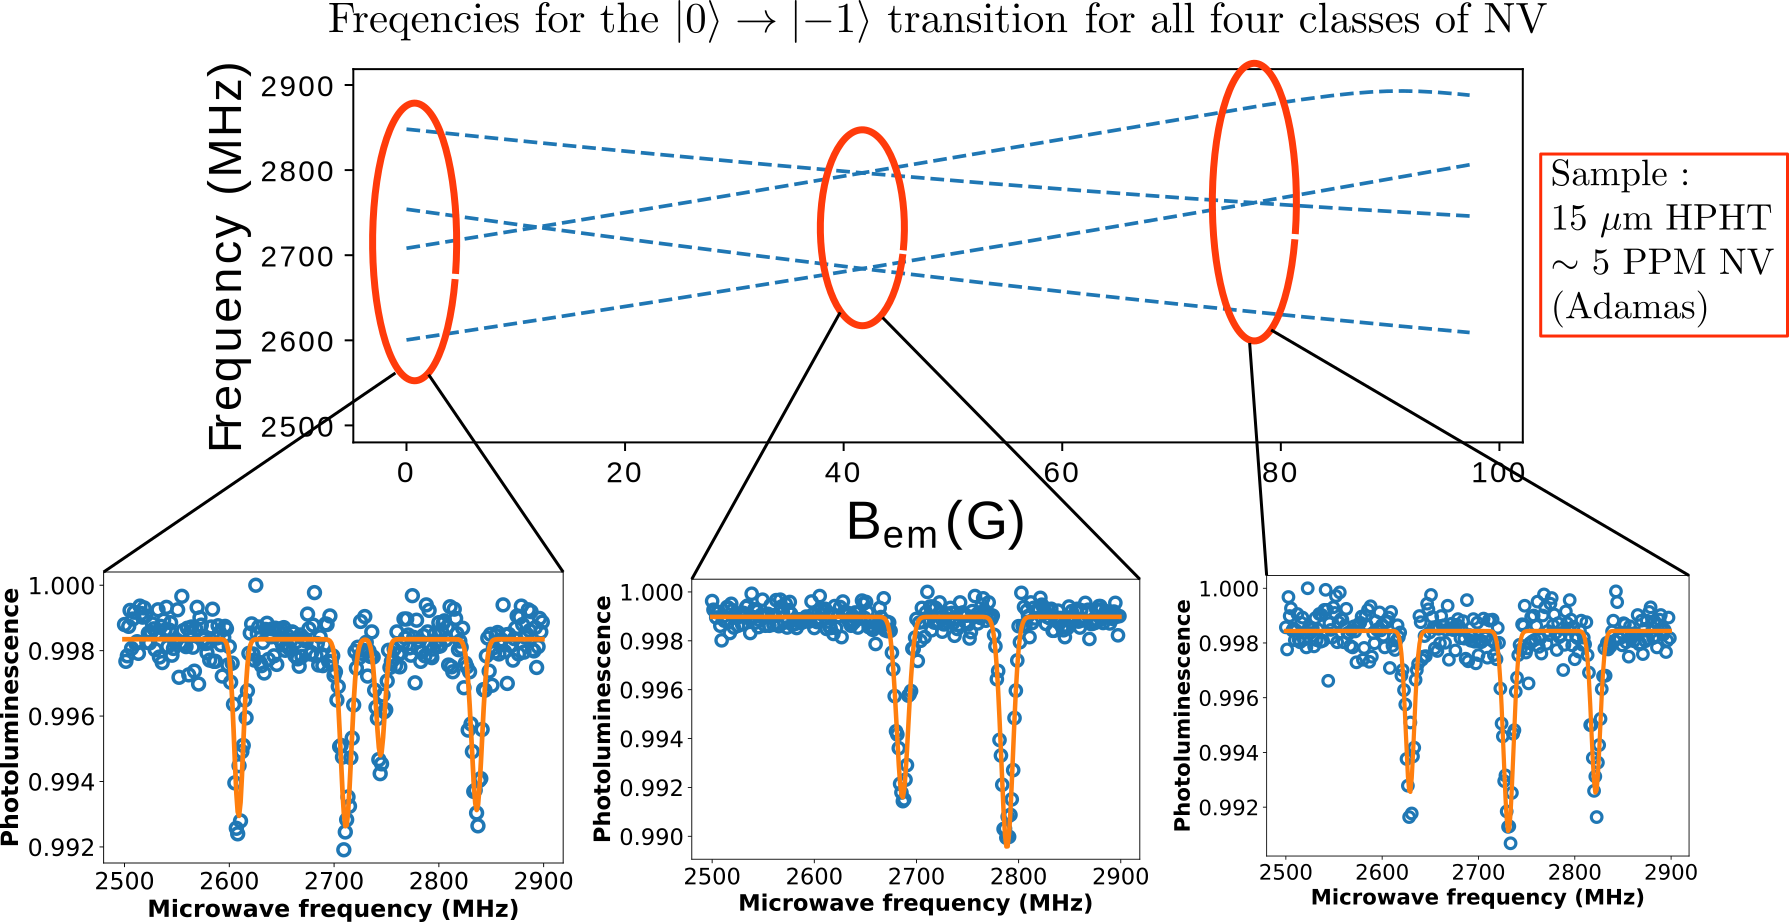
\includegraphics[scale=.24]{NV-NV_1}
    \onslide<2>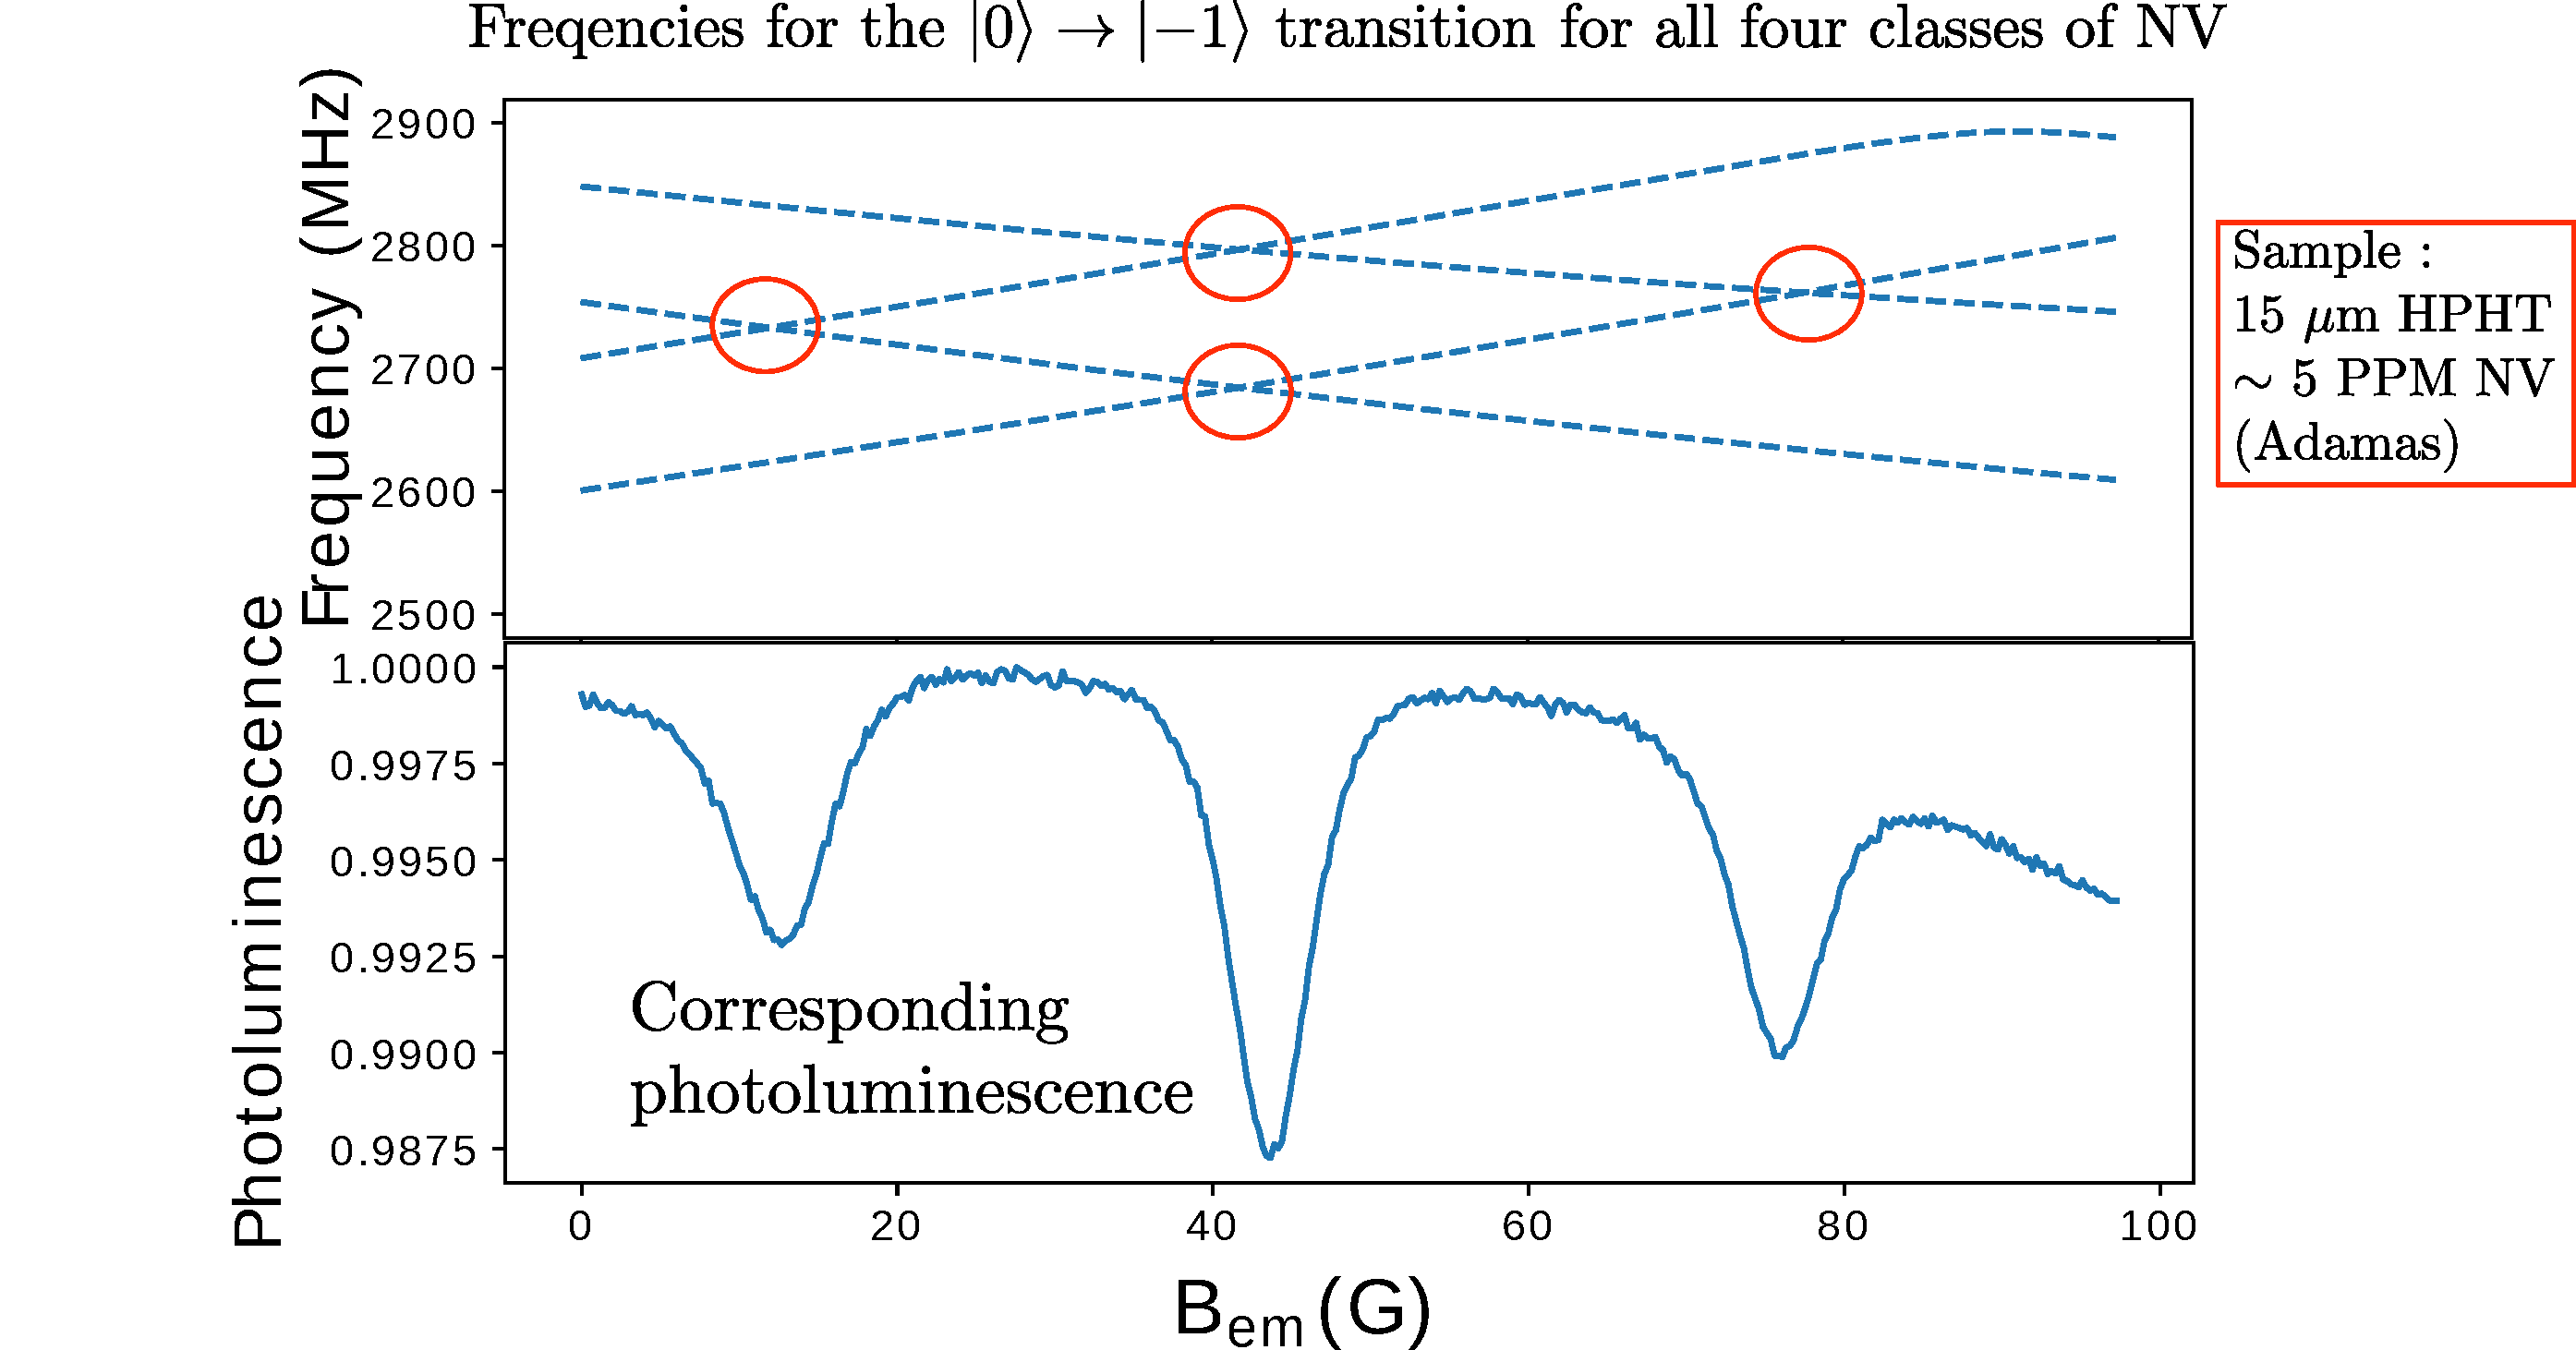
\includegraphics[scale=.24]{NV-NV_2}
    \end{overprint}
\end{figure}
\end{frame}
\begin{frame}{Explanation of the NV-NV cross-relaxations}
\fullcite{jarmola_temperature-_2012}

\fullcite{mrozek_longitudinal_2015}

\fullcite{choi_depolarization_2017}

\fullcite{giri_coupled_2018}

\fullcite{akhmedzhanov_magnetometry_2019}

\pause
\centering
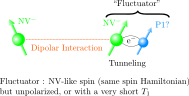
\includegraphics[scale=.35]{NVNV-micro_2}
\end{frame}
%ajouter la slide avec la carte du coup ?
\section{Mechanical detection of cross-relaxations with a levitating diamond}
\begin{frame}{Outline}
\tableofcontents[currentsection]
\end{frame}
\begin{frame}{Objectives of the experiment}
\begin{figure}
    \begin{overprint}
    \onslide<1>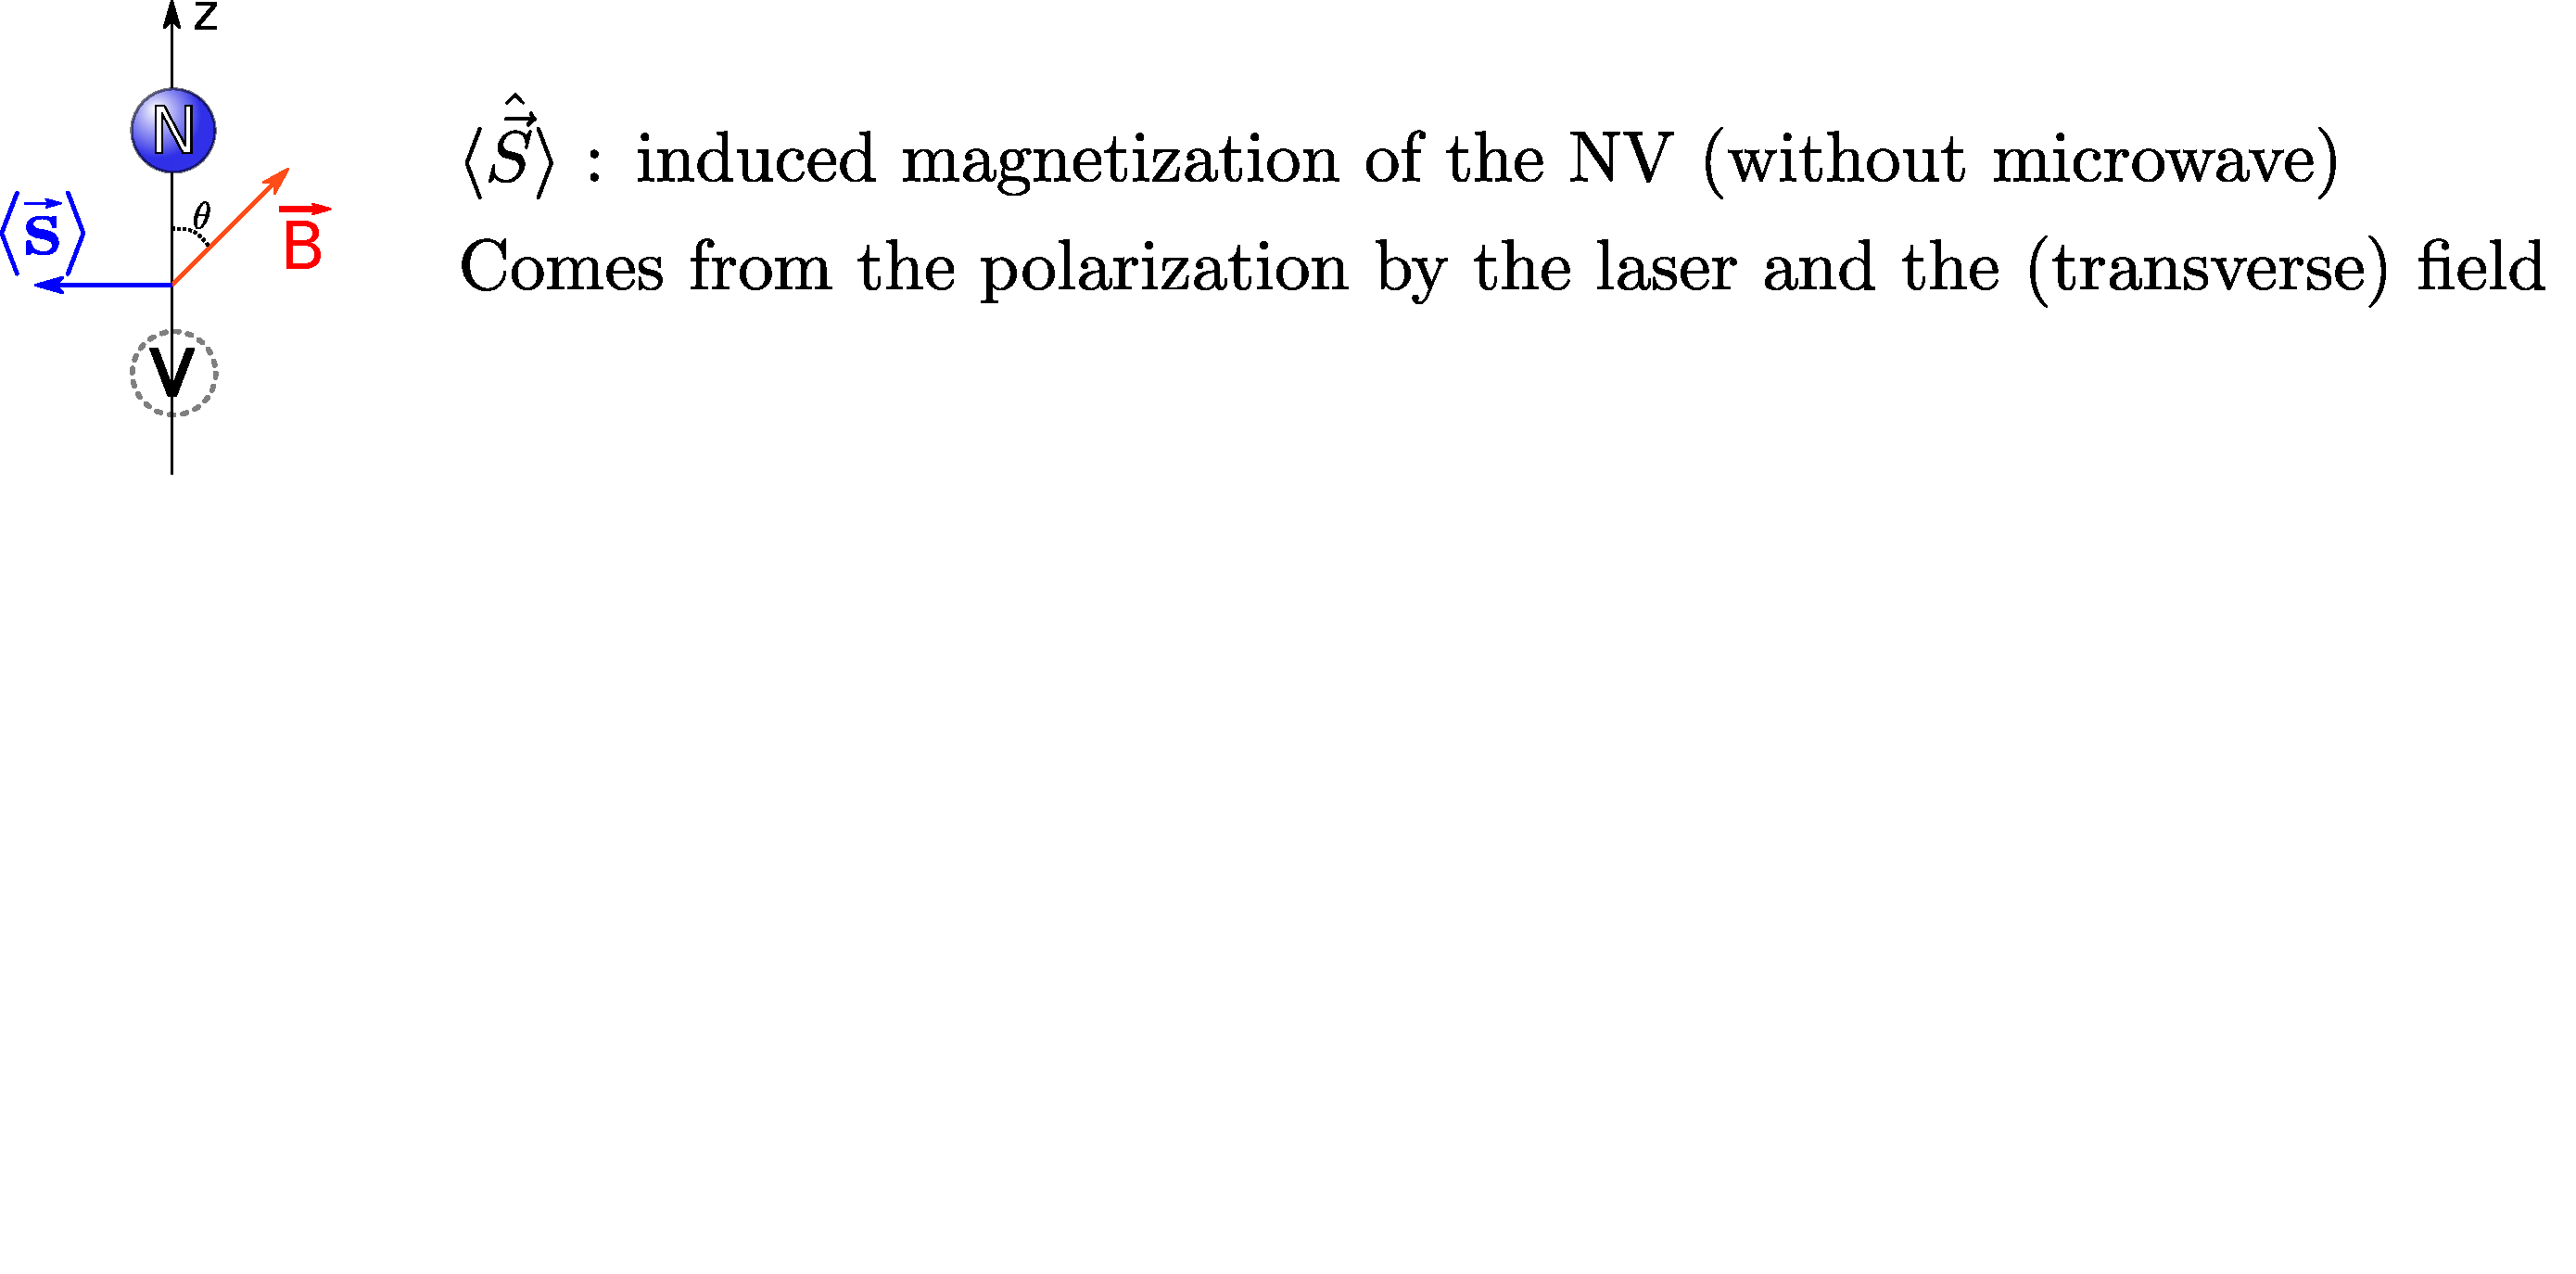
\includegraphics[scale=.23]{Explication_torque_alalouche_0}
    \onslide<2>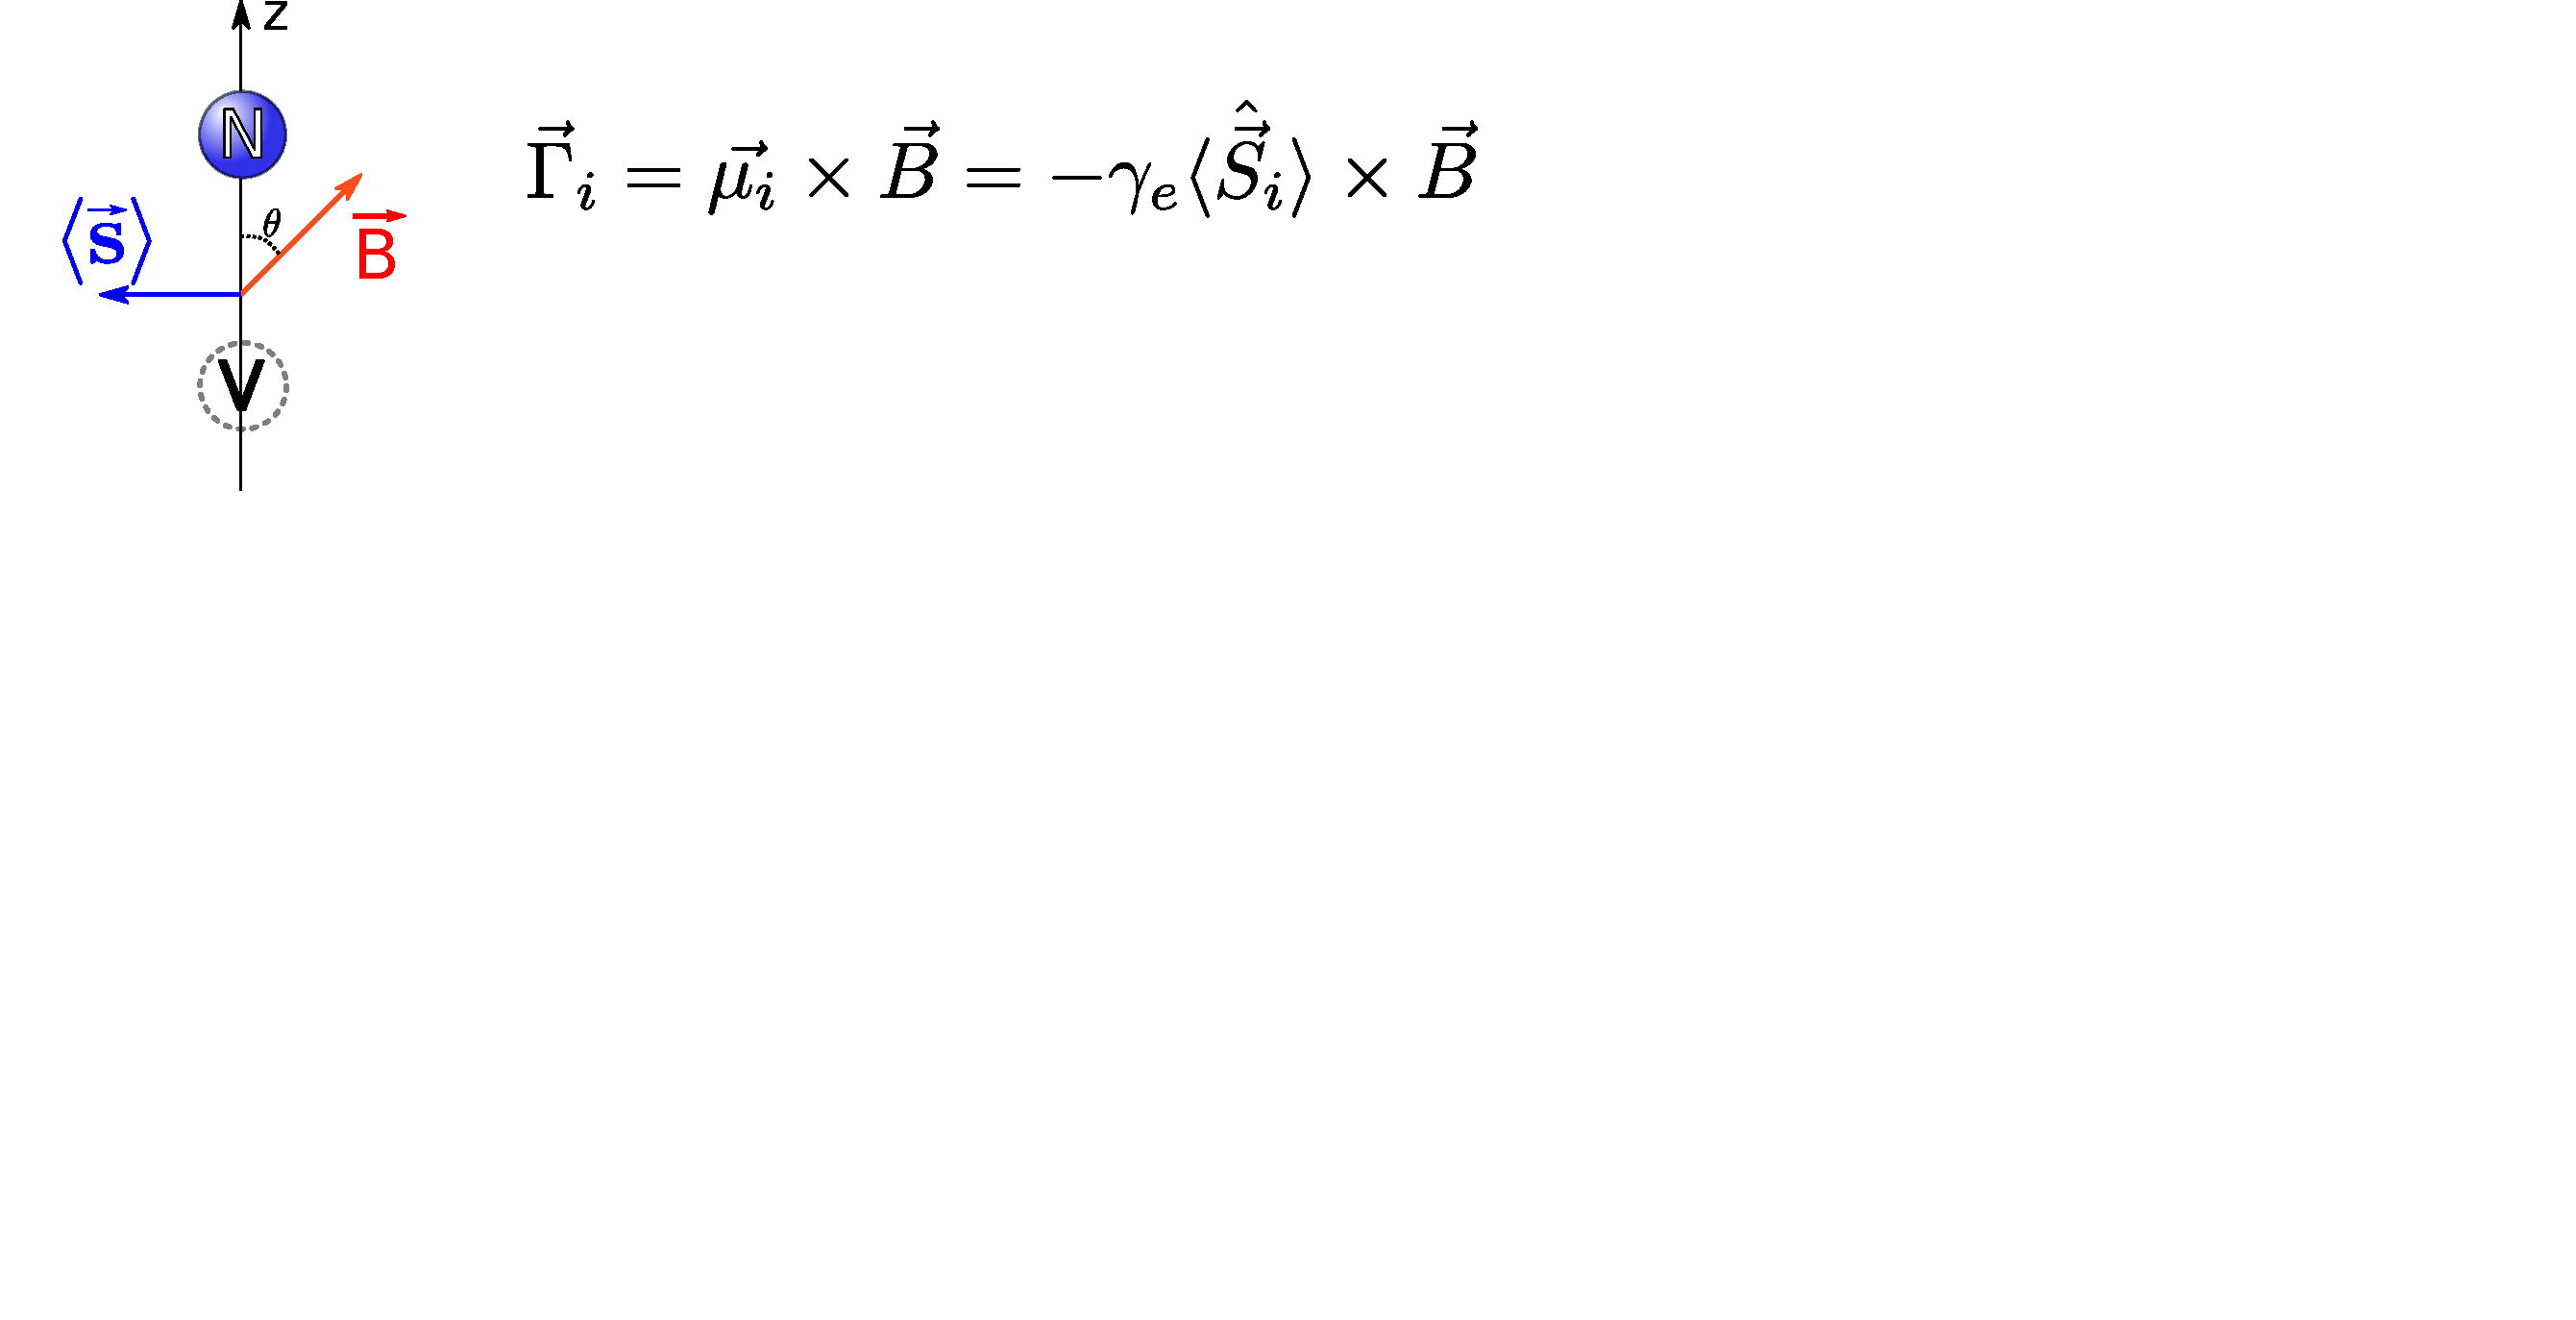
\includegraphics[scale=.23]{Explication_torque_alalouche_1}
    \onslide<3>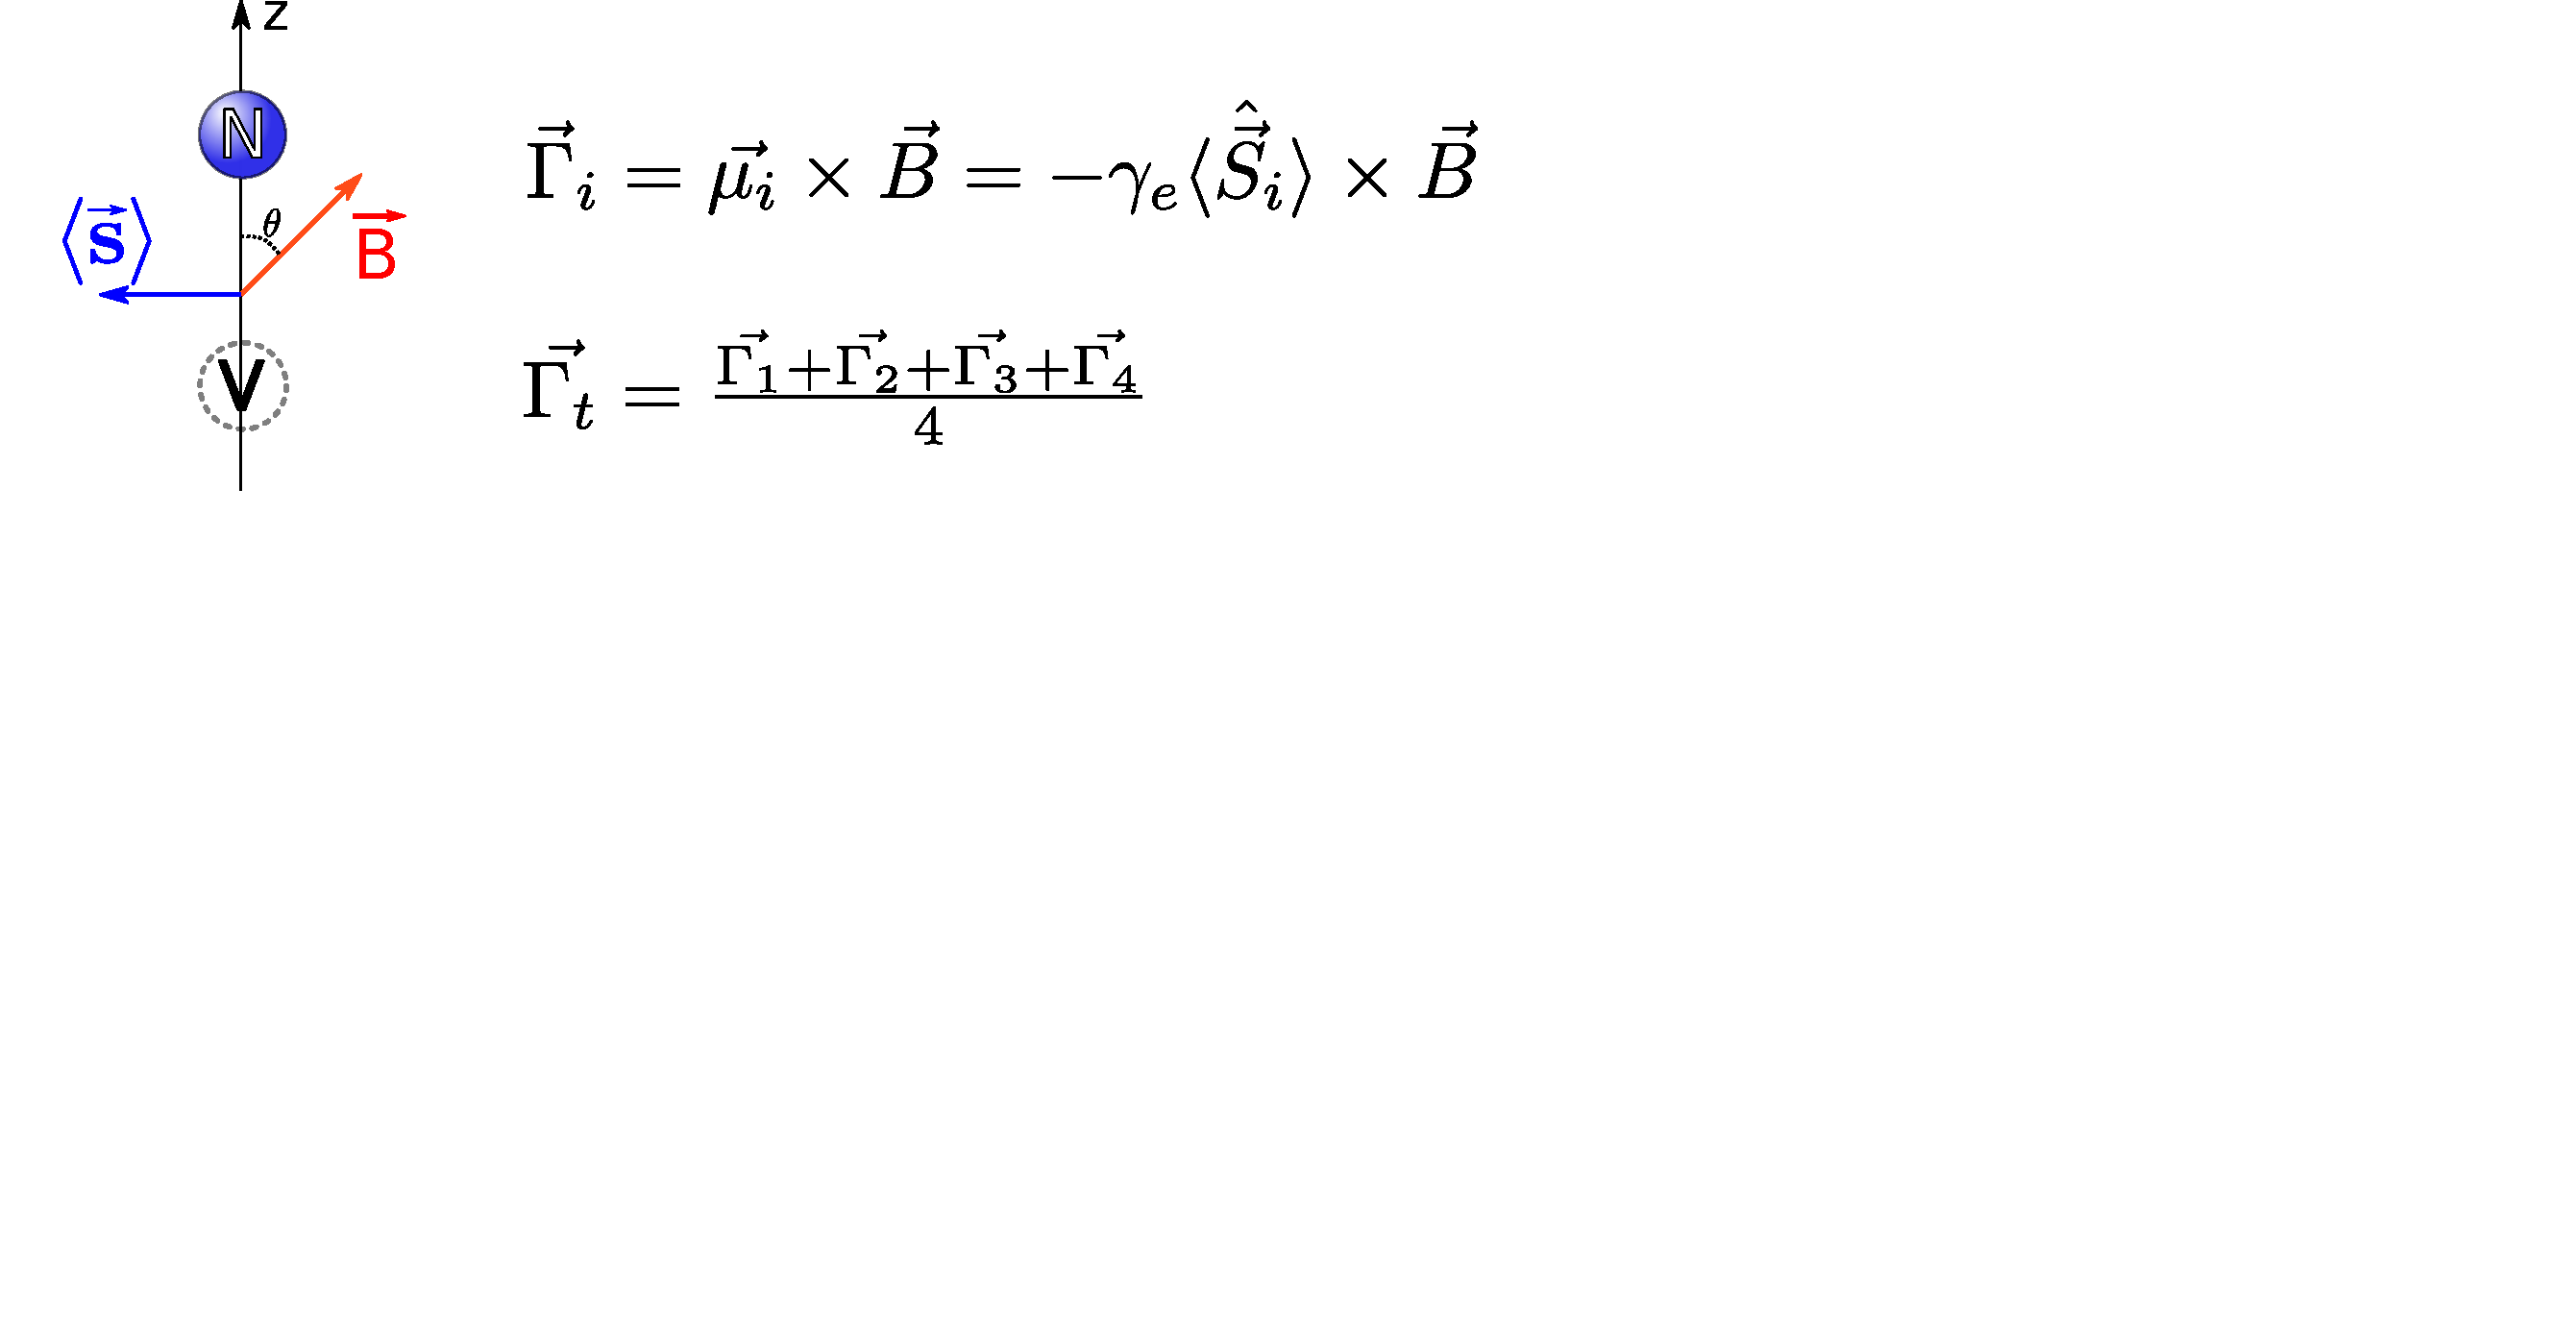
\includegraphics[scale=.23]{Explication_torque_alalouche_2}
    \onslide<4>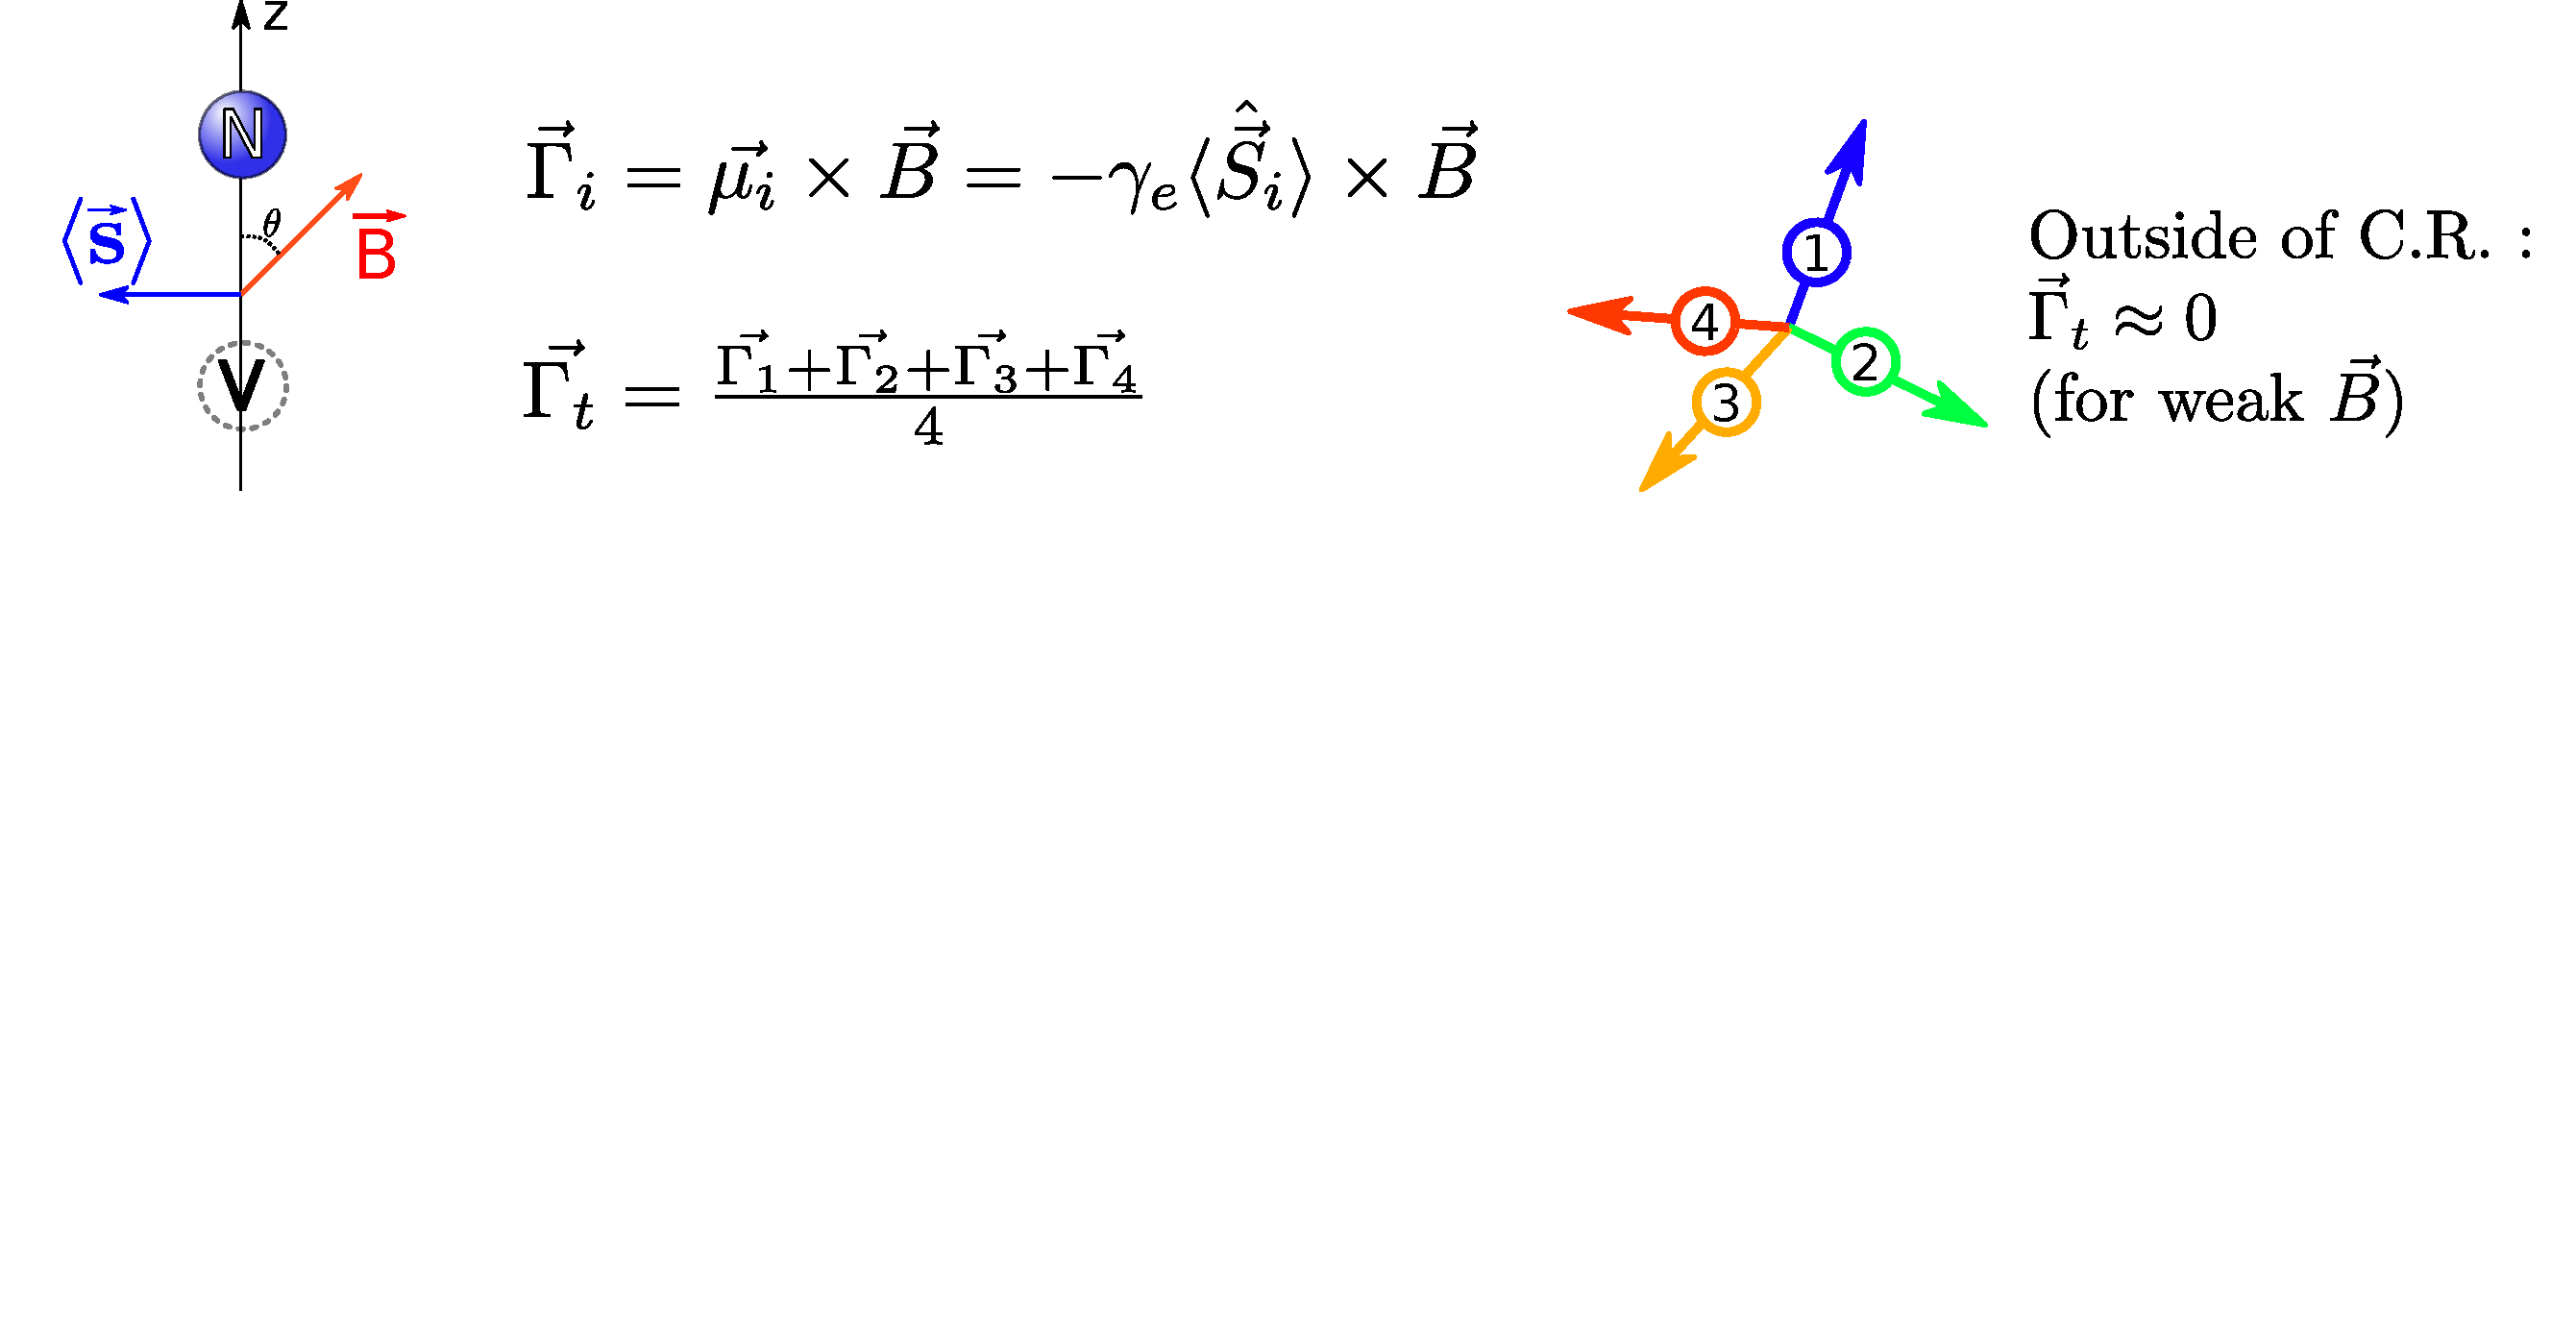
\includegraphics[scale=.23]{Explication_torque_alalouche_3}
    \onslide<5>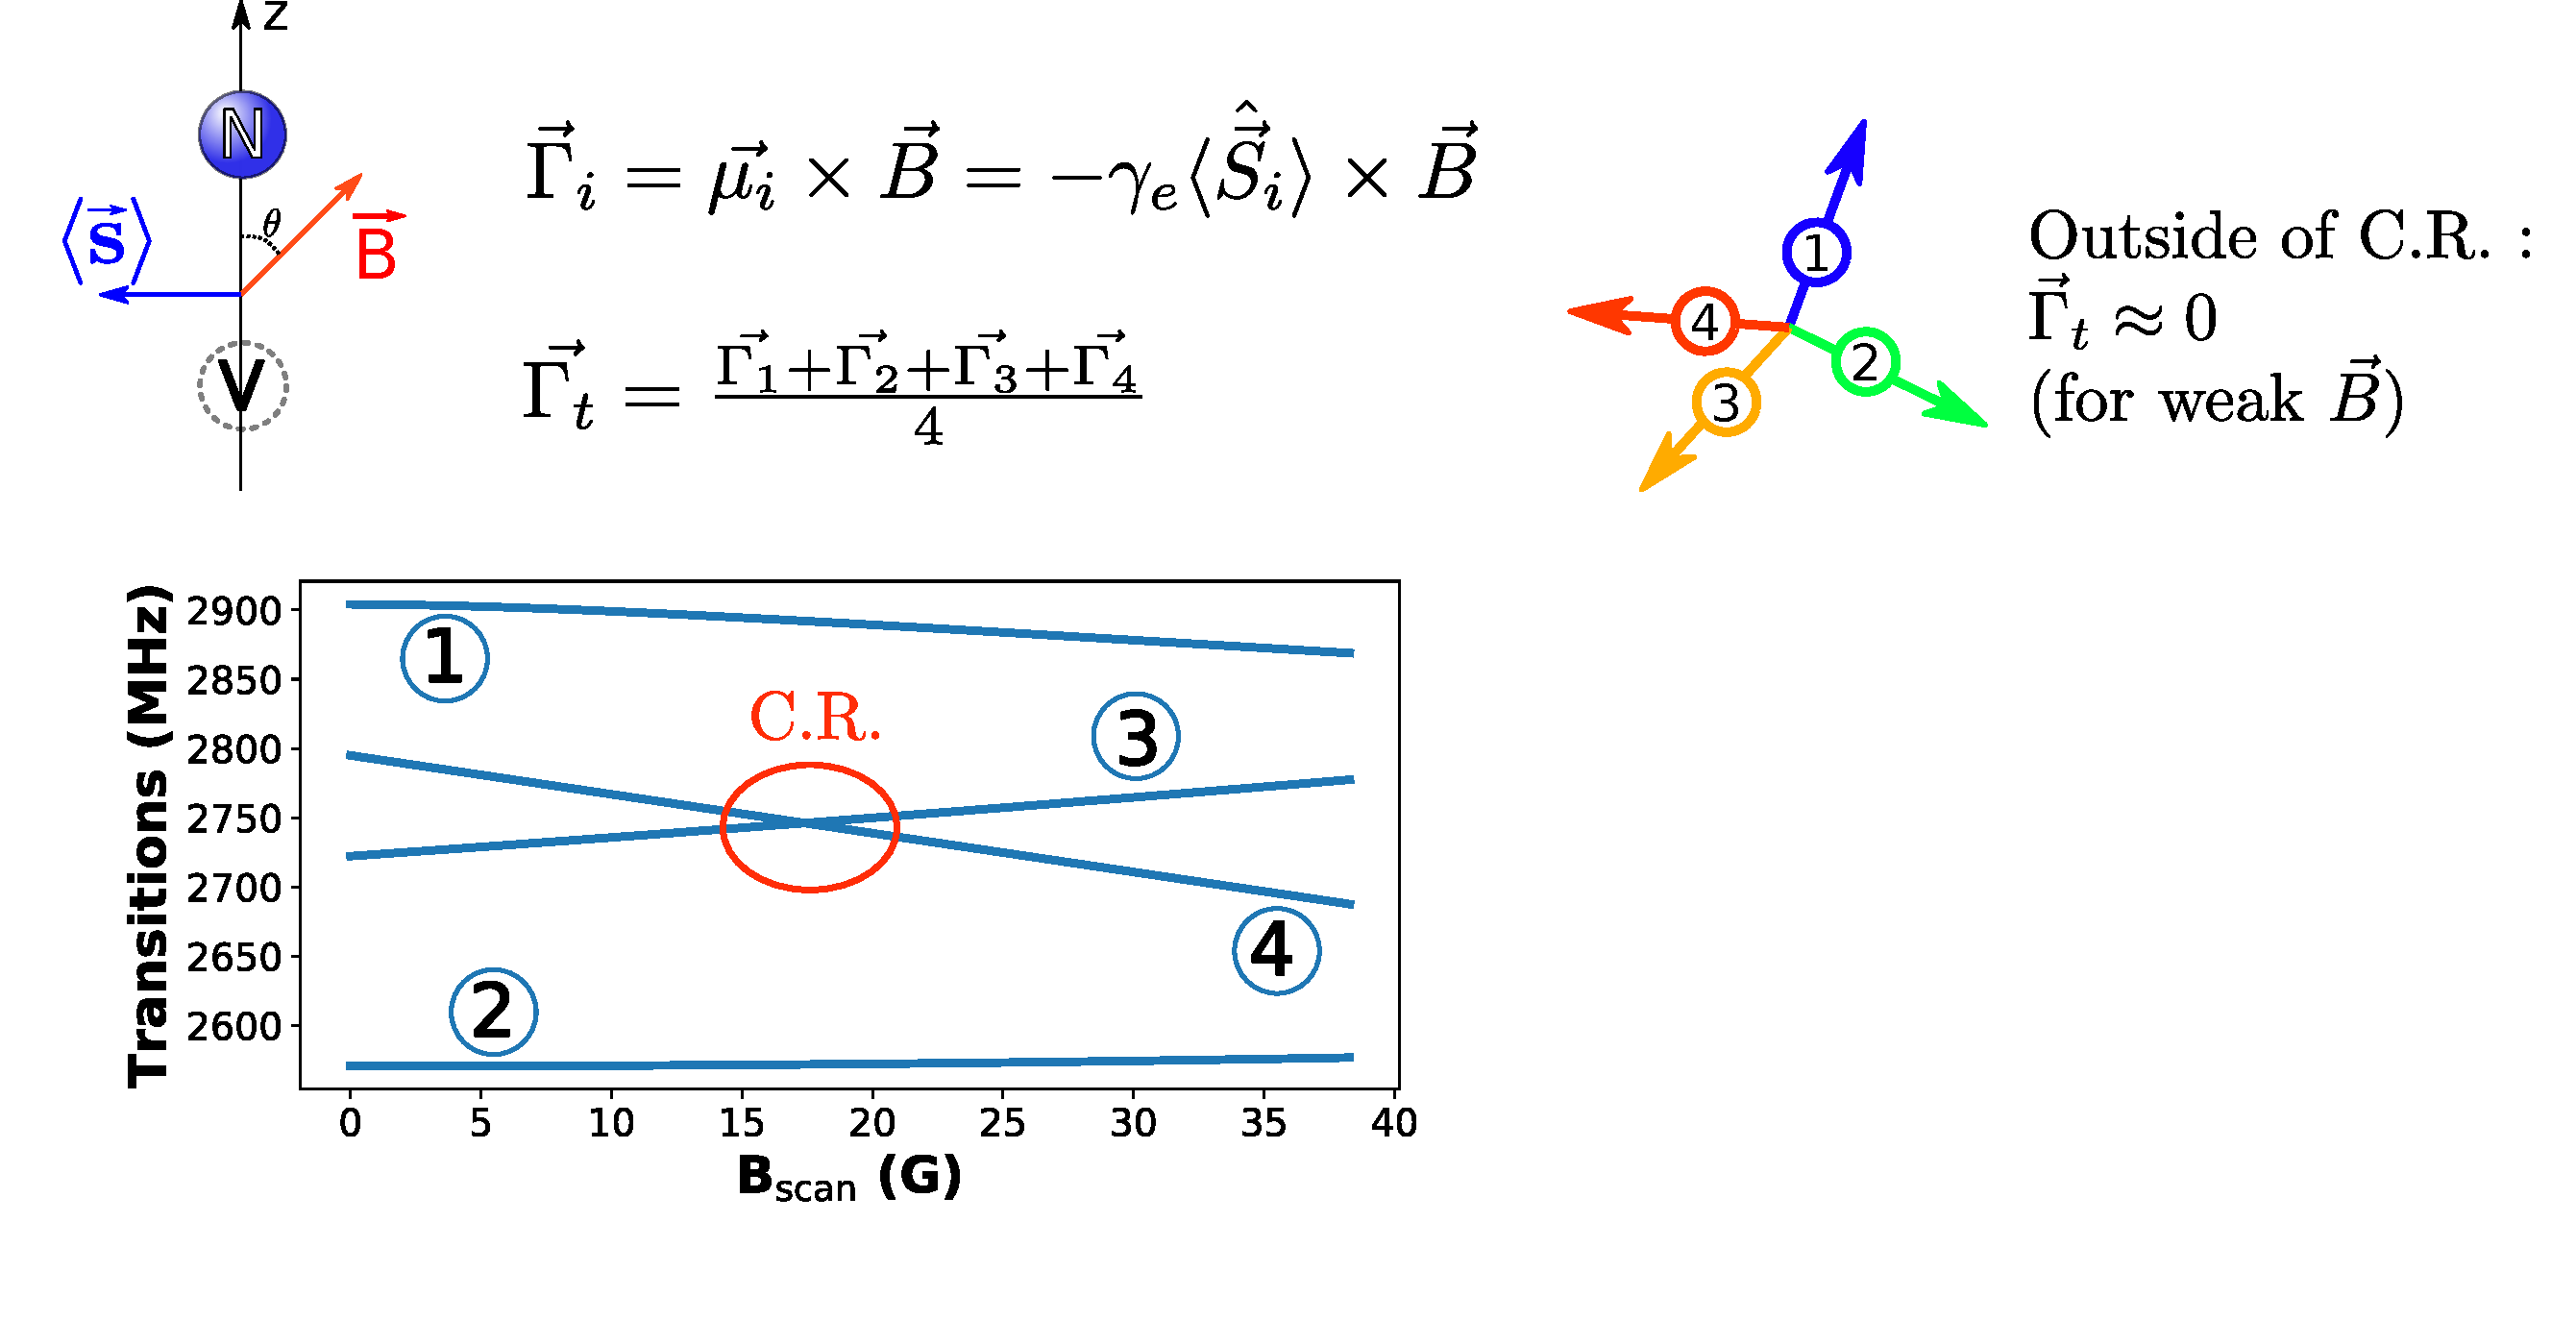
\includegraphics[scale=.23]{Explication_torque_alalouche_4}
    \onslide<6>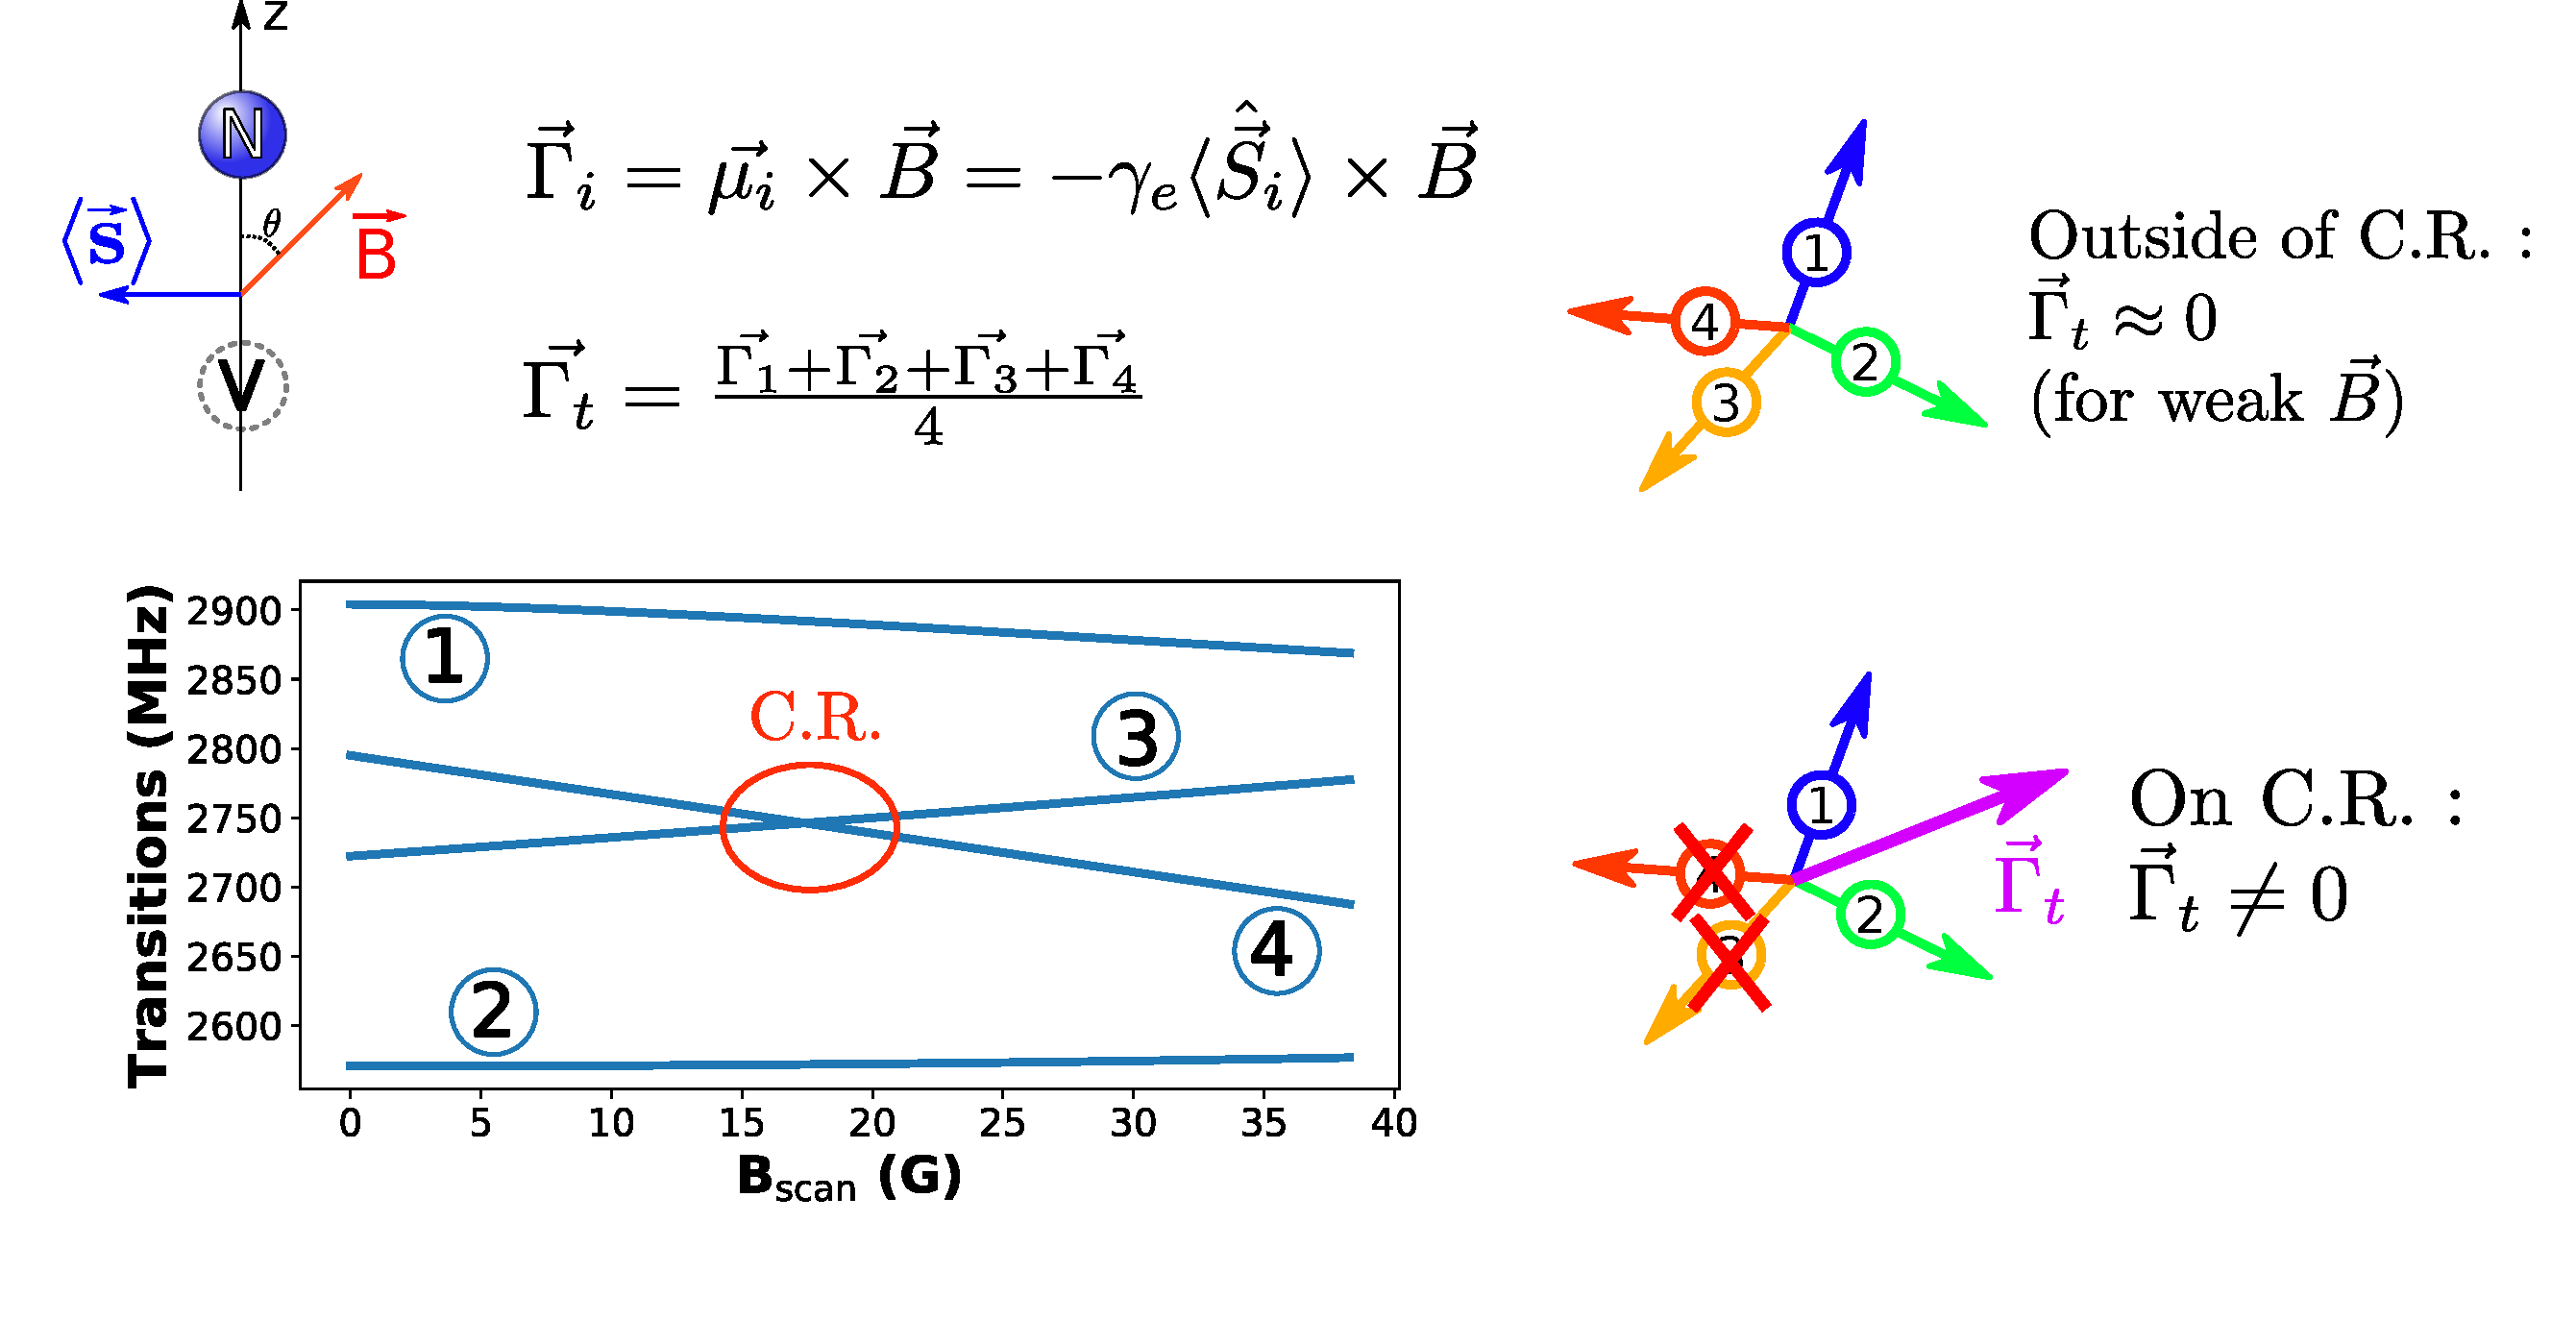
\includegraphics[scale=.23]{Explication_torque_alalouche_5}
    \end{overprint}
\end{figure}
\end{frame}
\begin{frame}{Torque measurement with a levitating diamond}
\centering
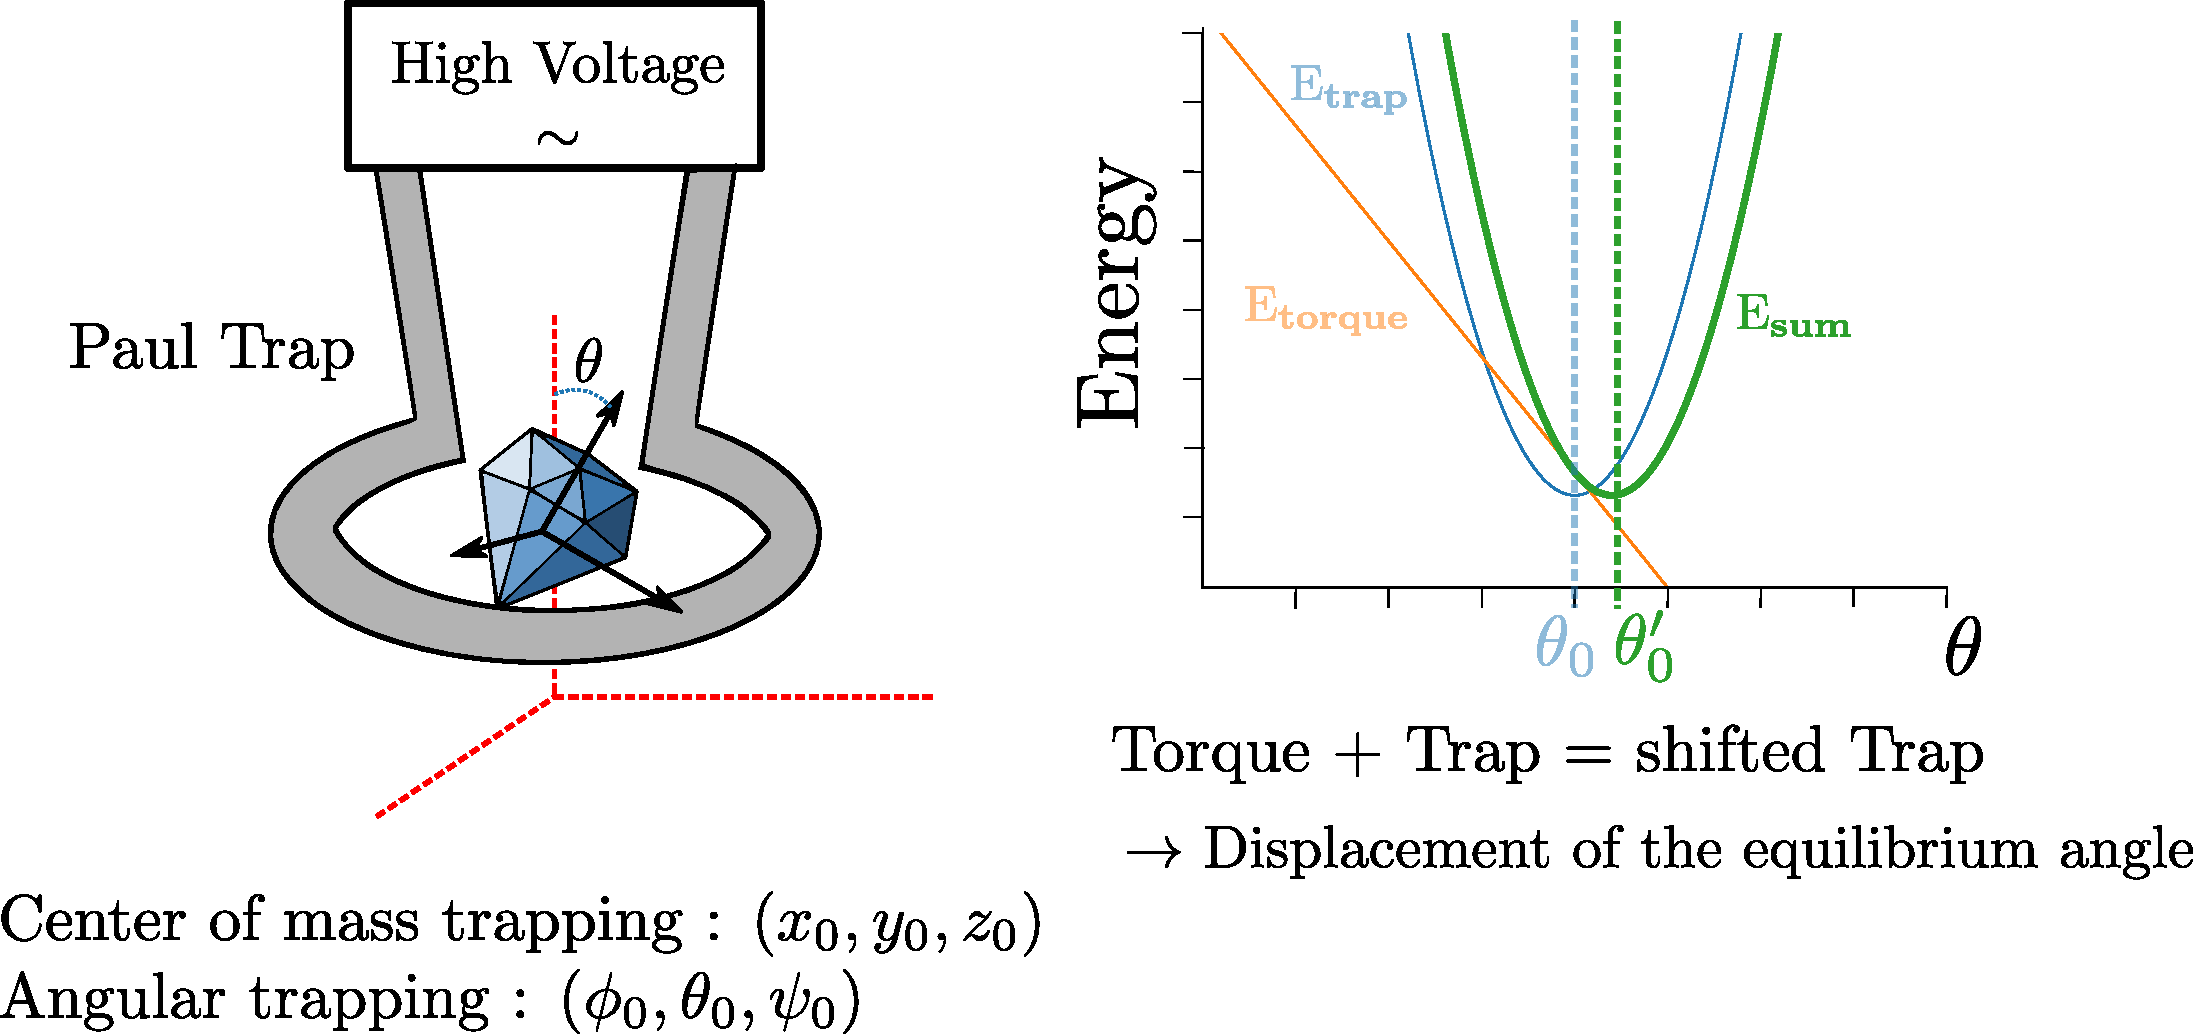
\includegraphics[scale=.3]{Trap_0}%"This trap not only locks the center of mass of the diamond, but it also locks its orientations, because of the anistropy of the trap and of the diamond" "The trap can be roughly modeled by an harmonic potential centered around a particular angle at equilibrium"
\end{frame}
\begin{frame}{Back-scattered laser detection}
\centering
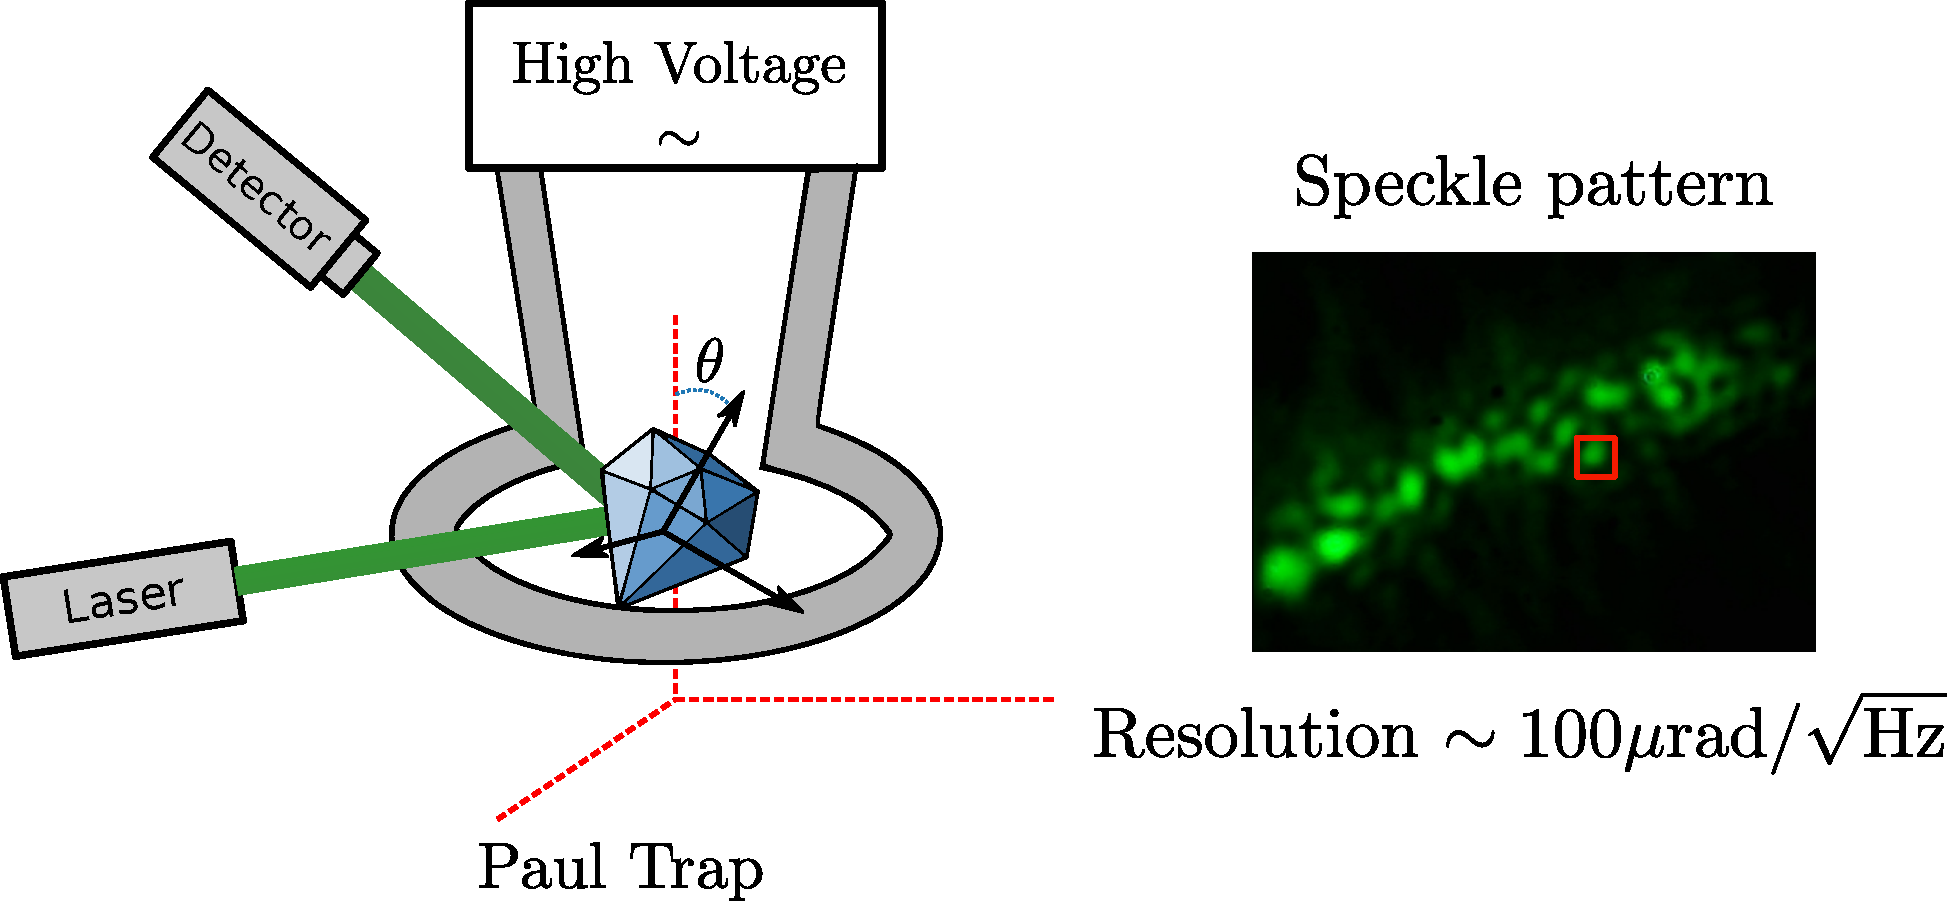
\includegraphics[scale=.085]{Trap_3}%And how do we measure this rotation ? well, since we have to send a laser on the diamond to polarise the NV centers..." "We do not observe a clear reflection of the laser, instead we observe a speckle pattern, which is produced by the many interferences on the rough surface of the diamond" "Whenever the diamond moves, the speckle pattern will either shift or change its shape..."
\end{frame}
\begin{frame}{Measurement of the torque caused by C.R.}
\begin{figure}
    \begin{overprint}
    \onslide<1>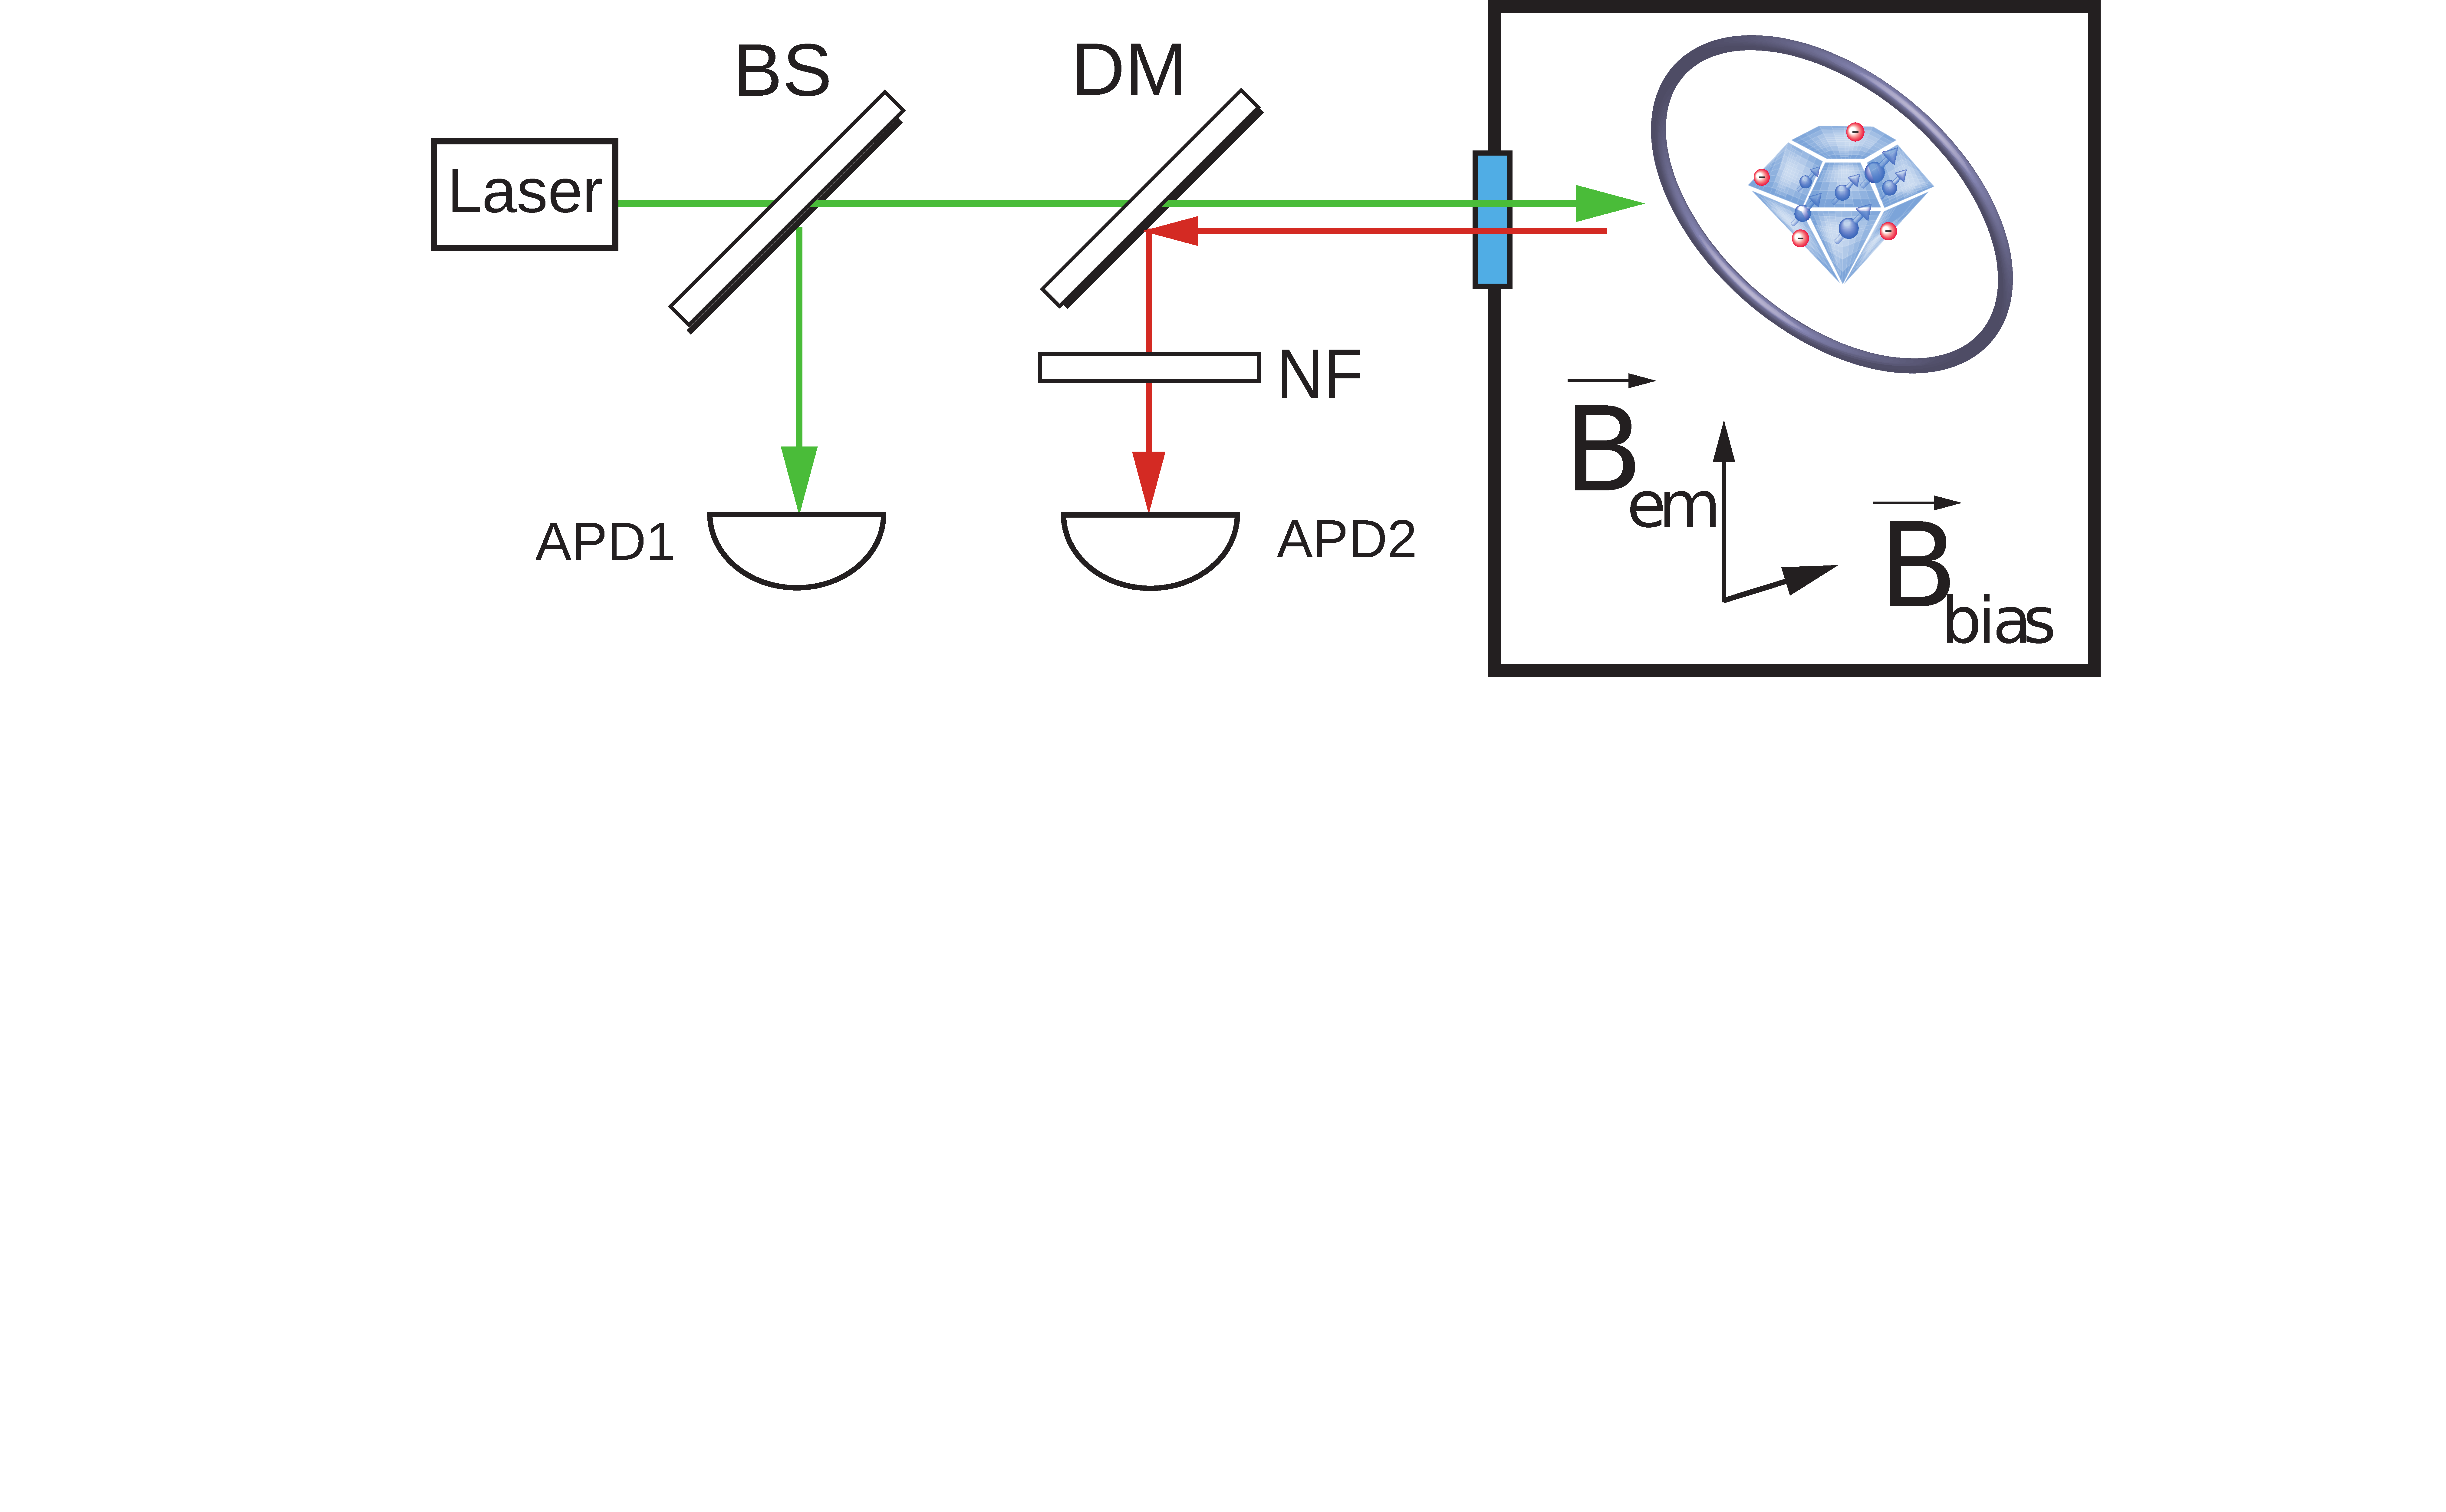
\includegraphics[scale=.08]{CRmeca_121_mieux_0}
    \onslide<2>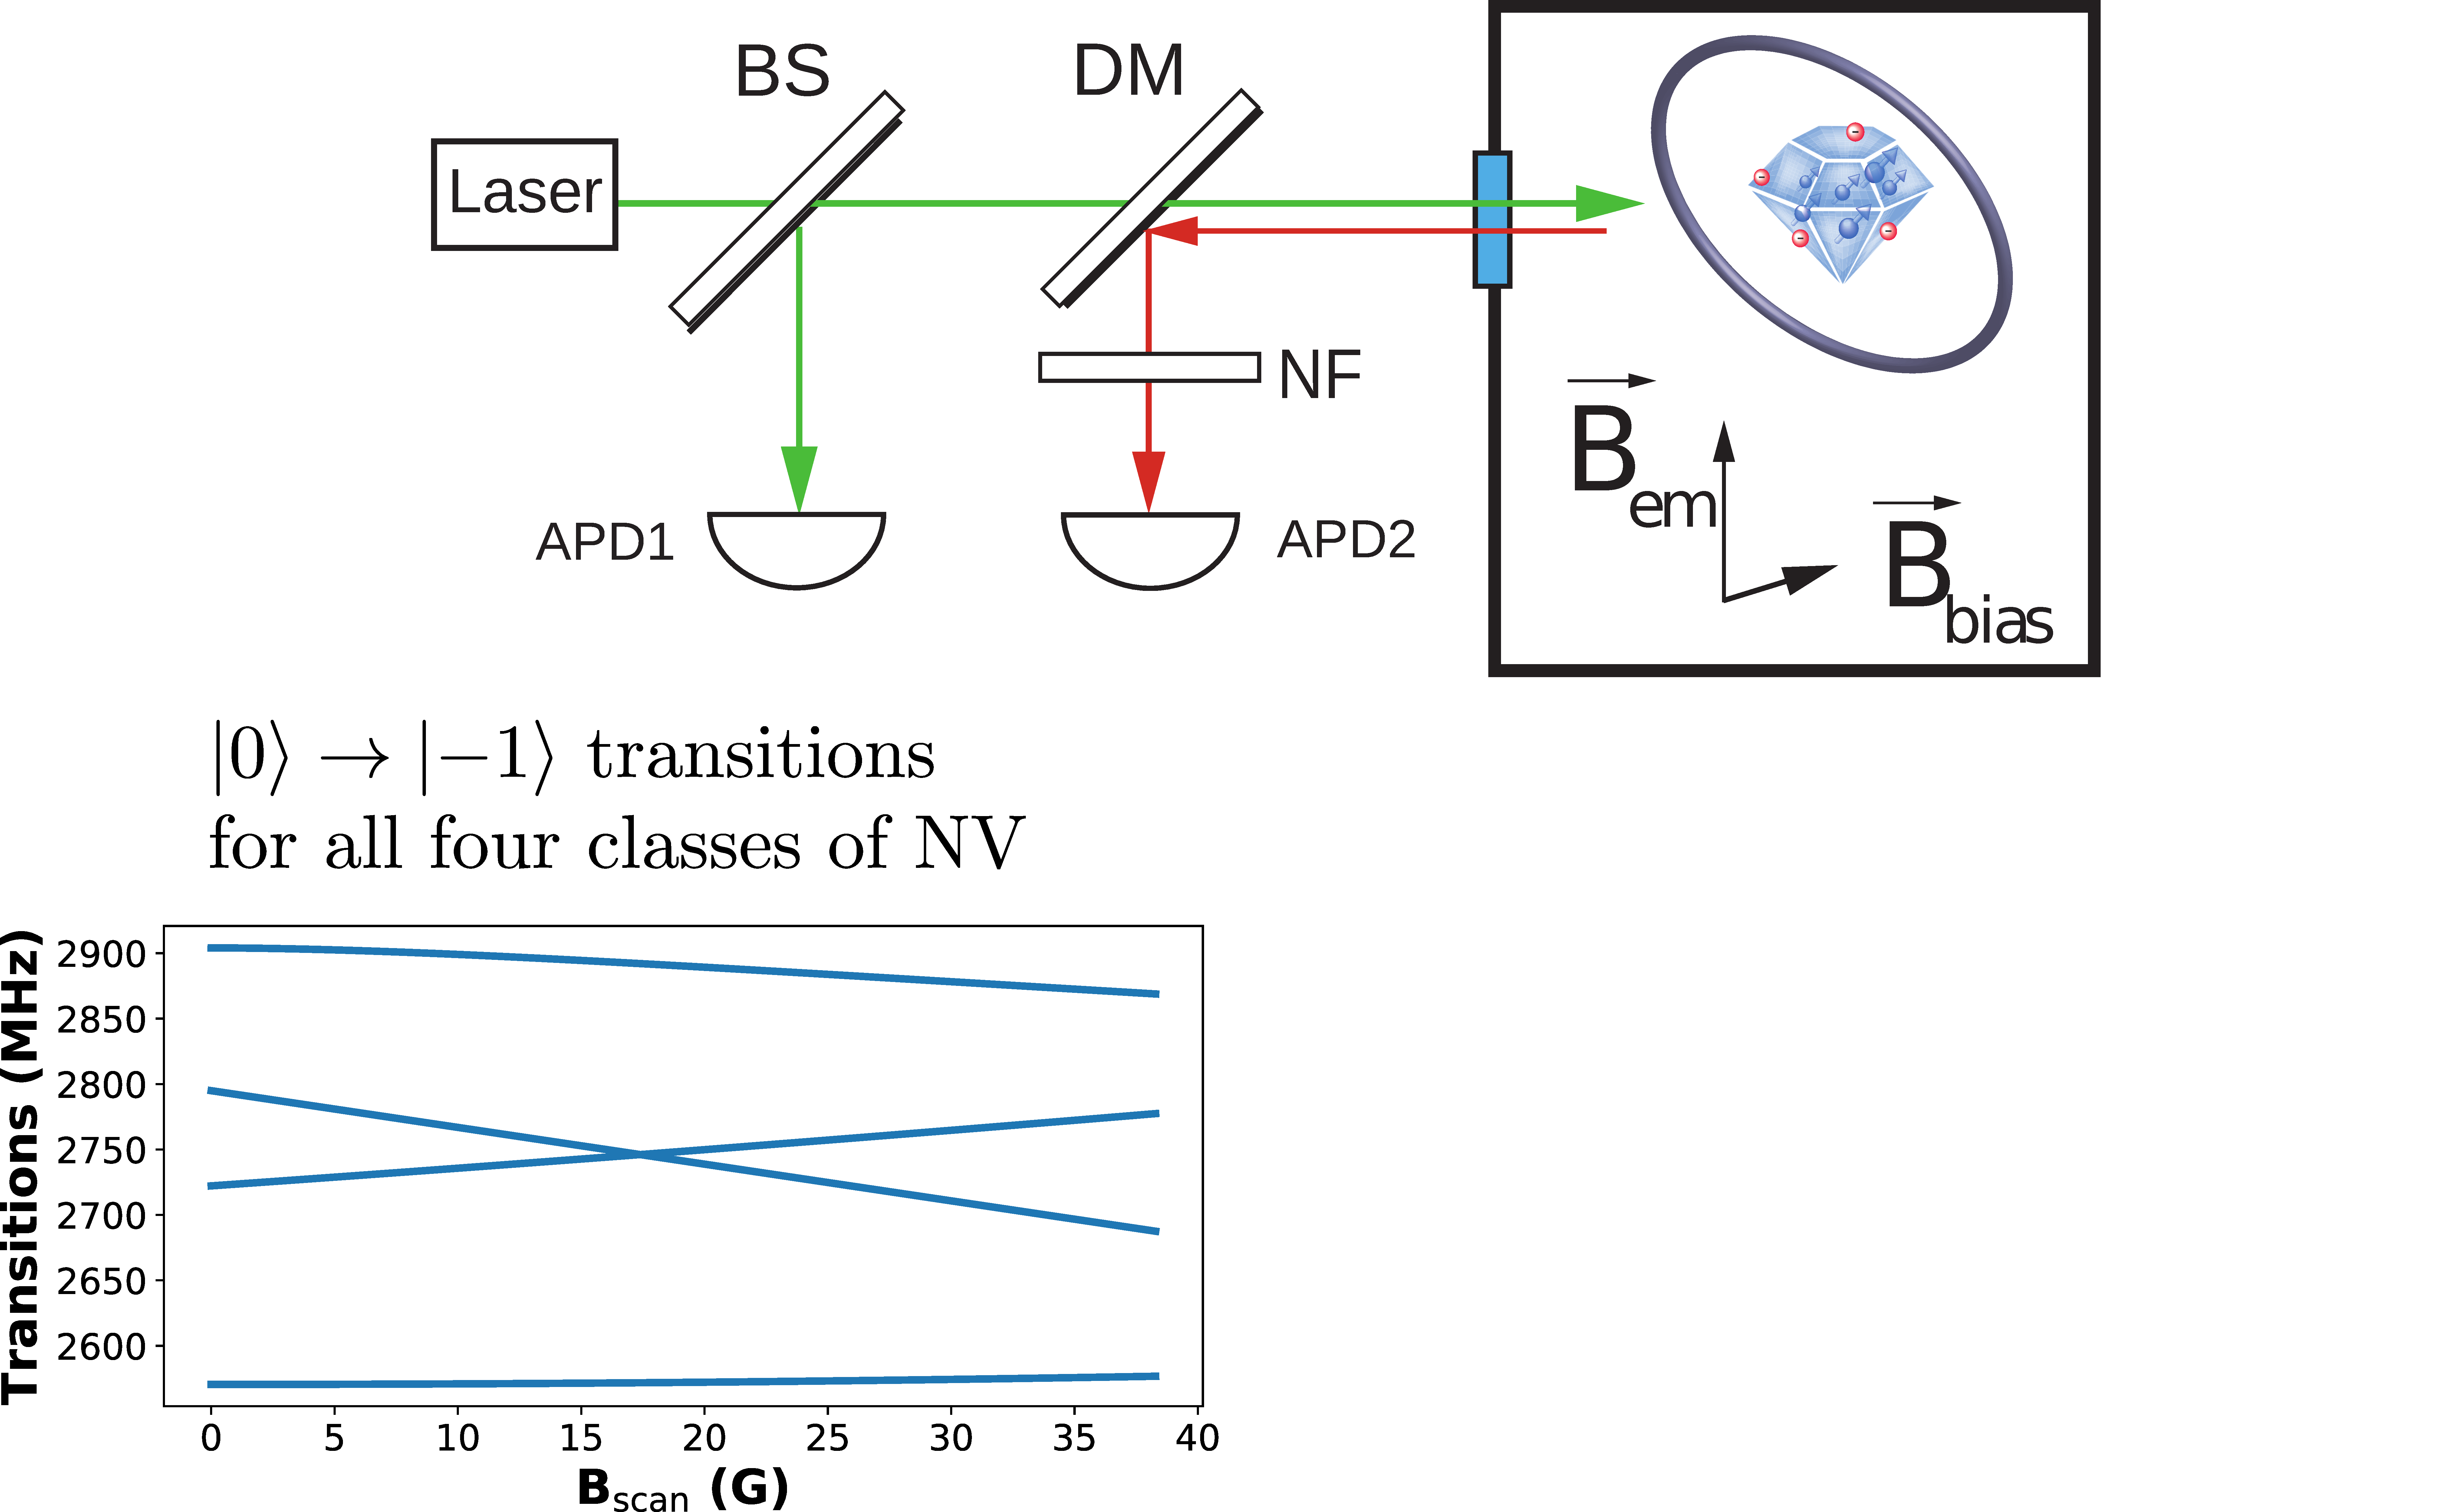
\includegraphics[scale=.08]{CRmeca_121_mieux_1}
    \onslide<3>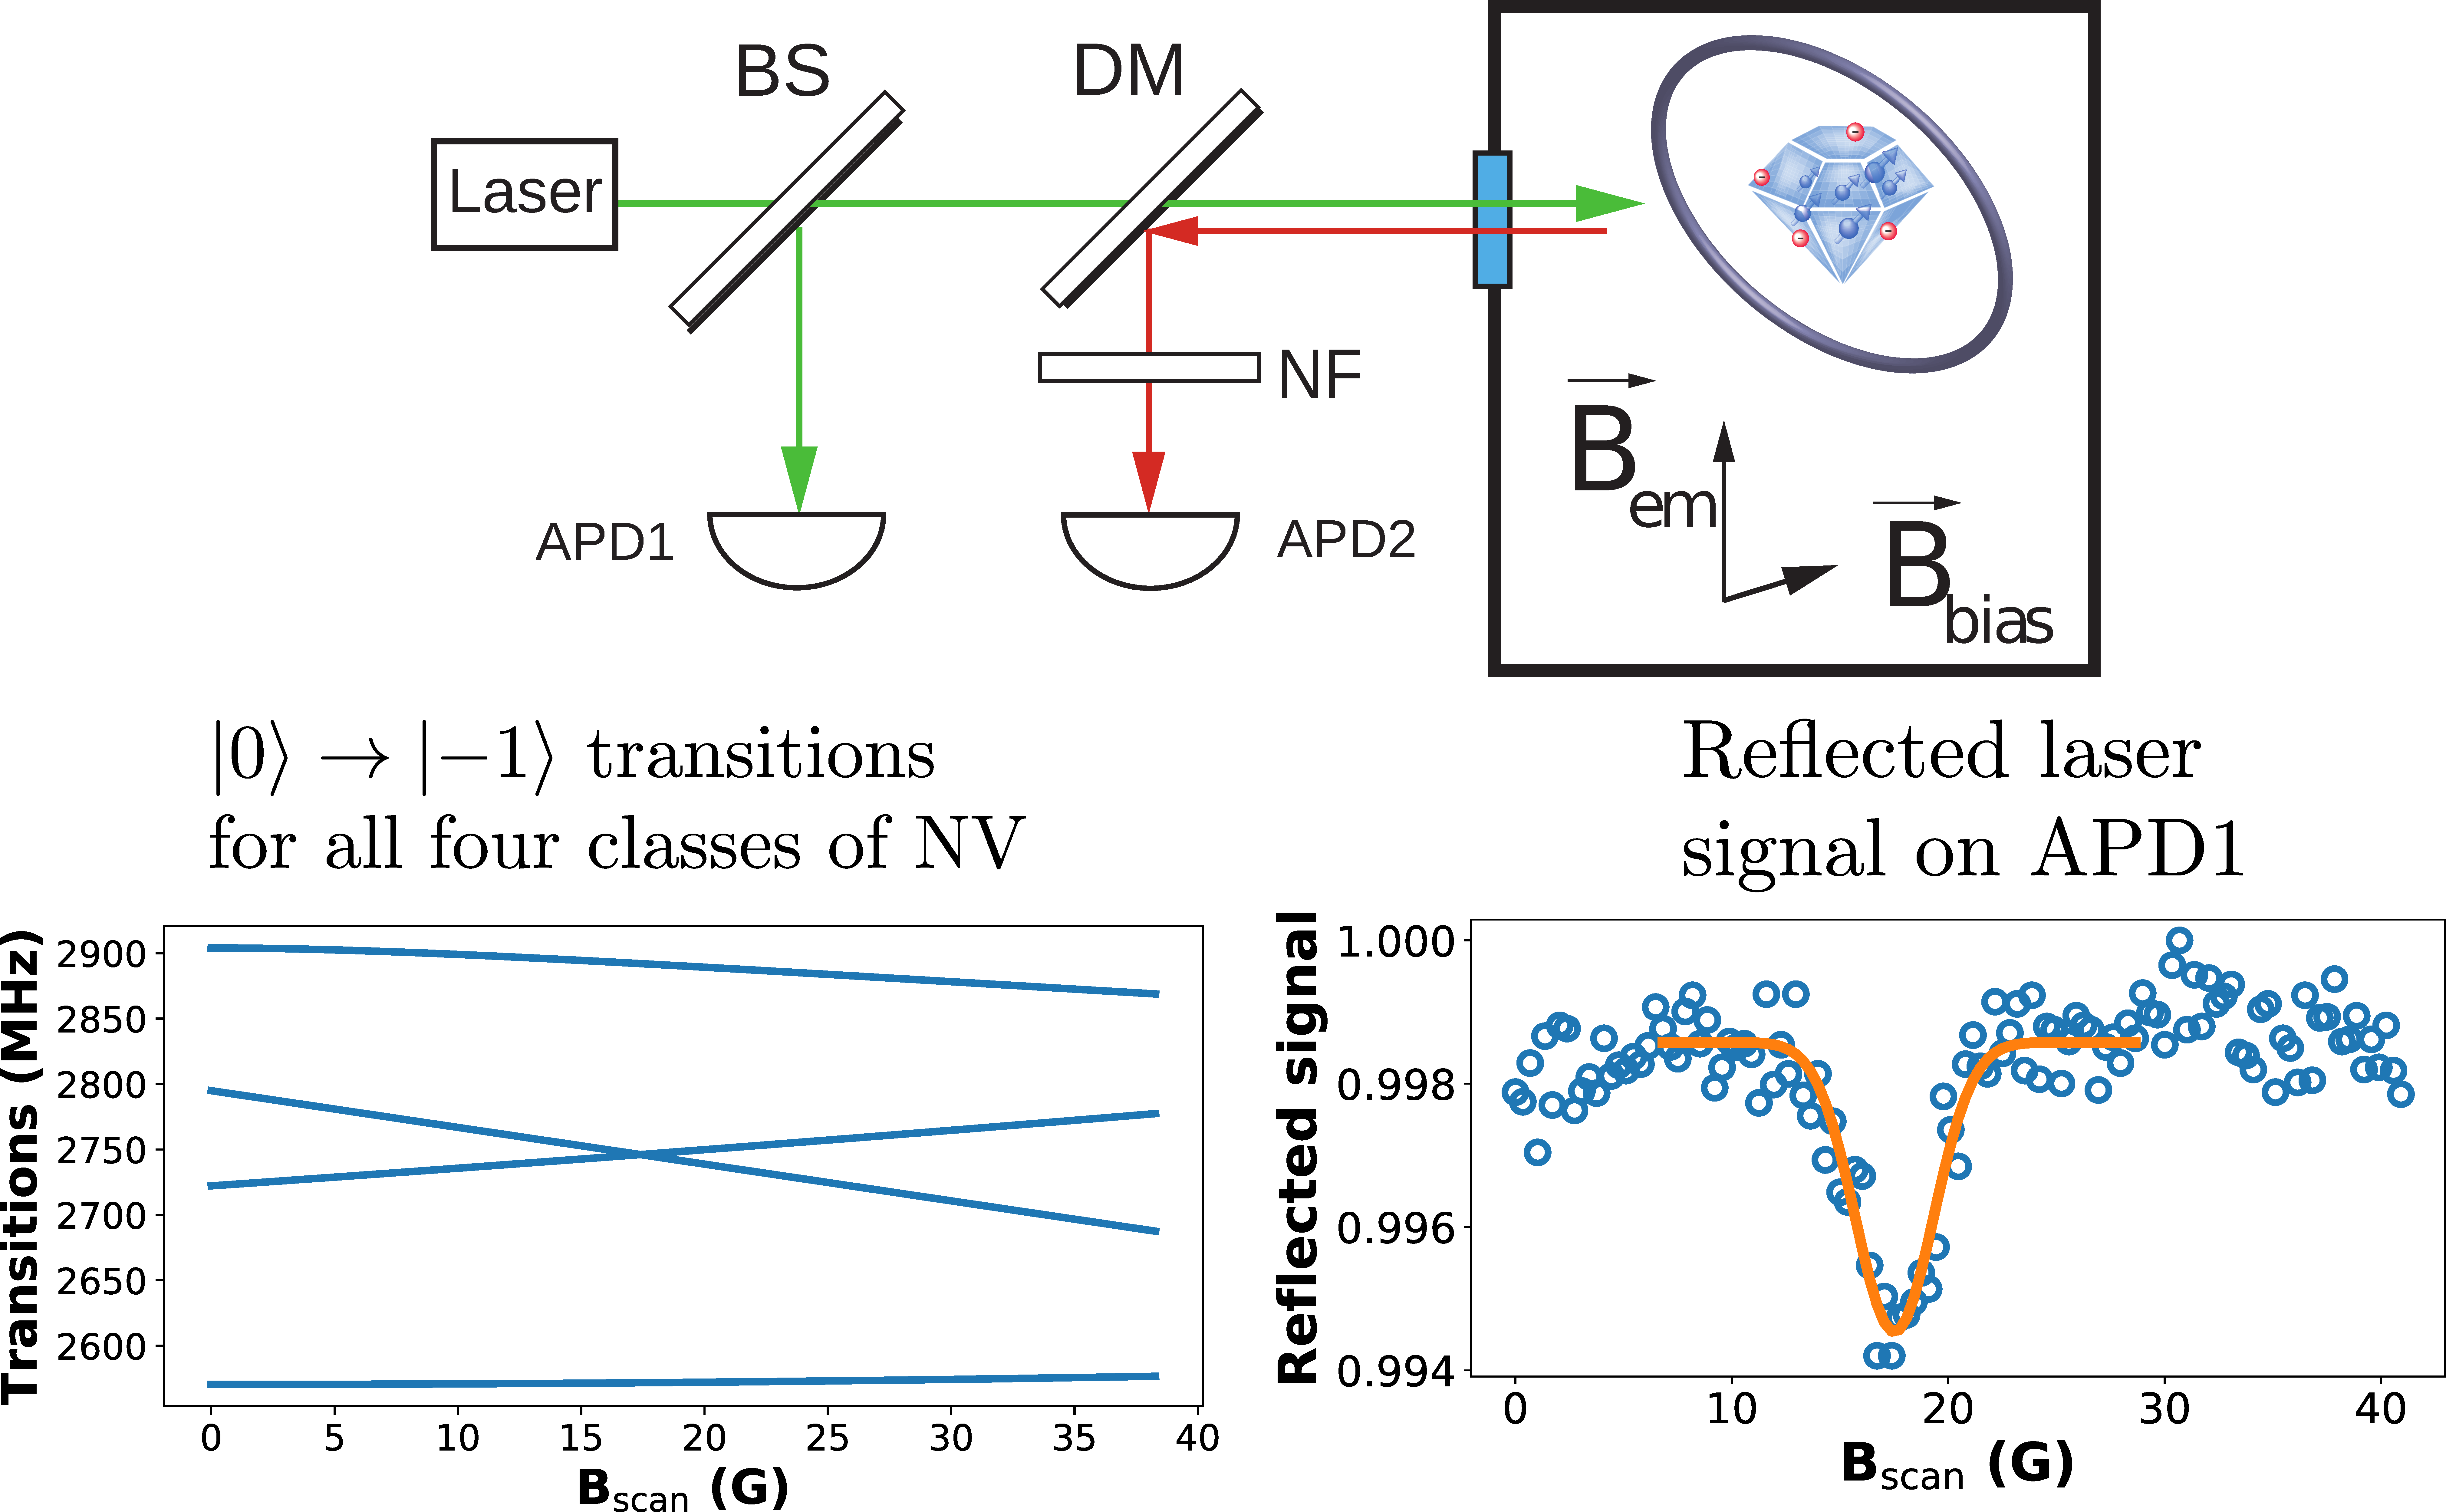
\includegraphics[scale=.08]{CRmeca_121_mieux_2}
    \end{overprint}
\end{figure}
\end{frame}
\begin{frame}{Conclusion}
\begin{tcolorbox}[title=Summary,colbacktitle=red!80!white]
\begin{itemize}
\item{Optical detection of new spin defects in CVD diamond through cross-relaxations with NV centers}
\item{Mechanical detection of NV induced magnetization enhanced by cross-relaxations}
\end{itemize}
\end{tcolorbox}
\pause
\begin{tcolorbox}[title=Prospects,colbacktitle=blue!80!white]
Observation of cross-relaxation between NV and another spin in a levitating (CVD ?) diamond.
\begin{itemize}
\item Mechanical detection of a non-NV spin thanks to hyperpolarization
\item Angular momentum conservation with non-spin preserving dipolar coupling (Einstein-de Haas effect)
\end{itemize}
\end{tcolorbox}
\end{frame}
\begin{frame}{Cross-relaxation between NV$^-$ and $^{13}$C$-$NV$^-$}
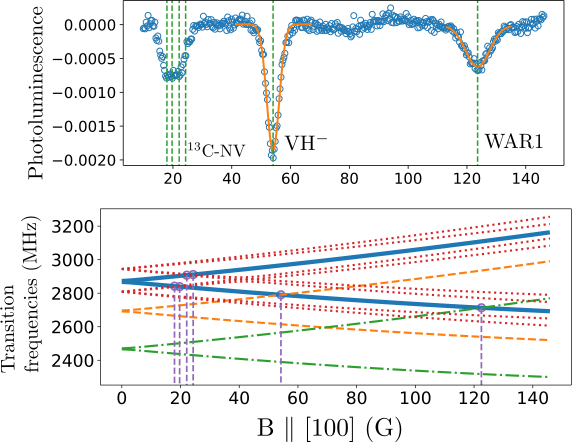
\includegraphics[scale=.45]{soustraction_3}
\end{frame}
\begin{frame}{Simulation of the C.R.-caused torque}
\centering
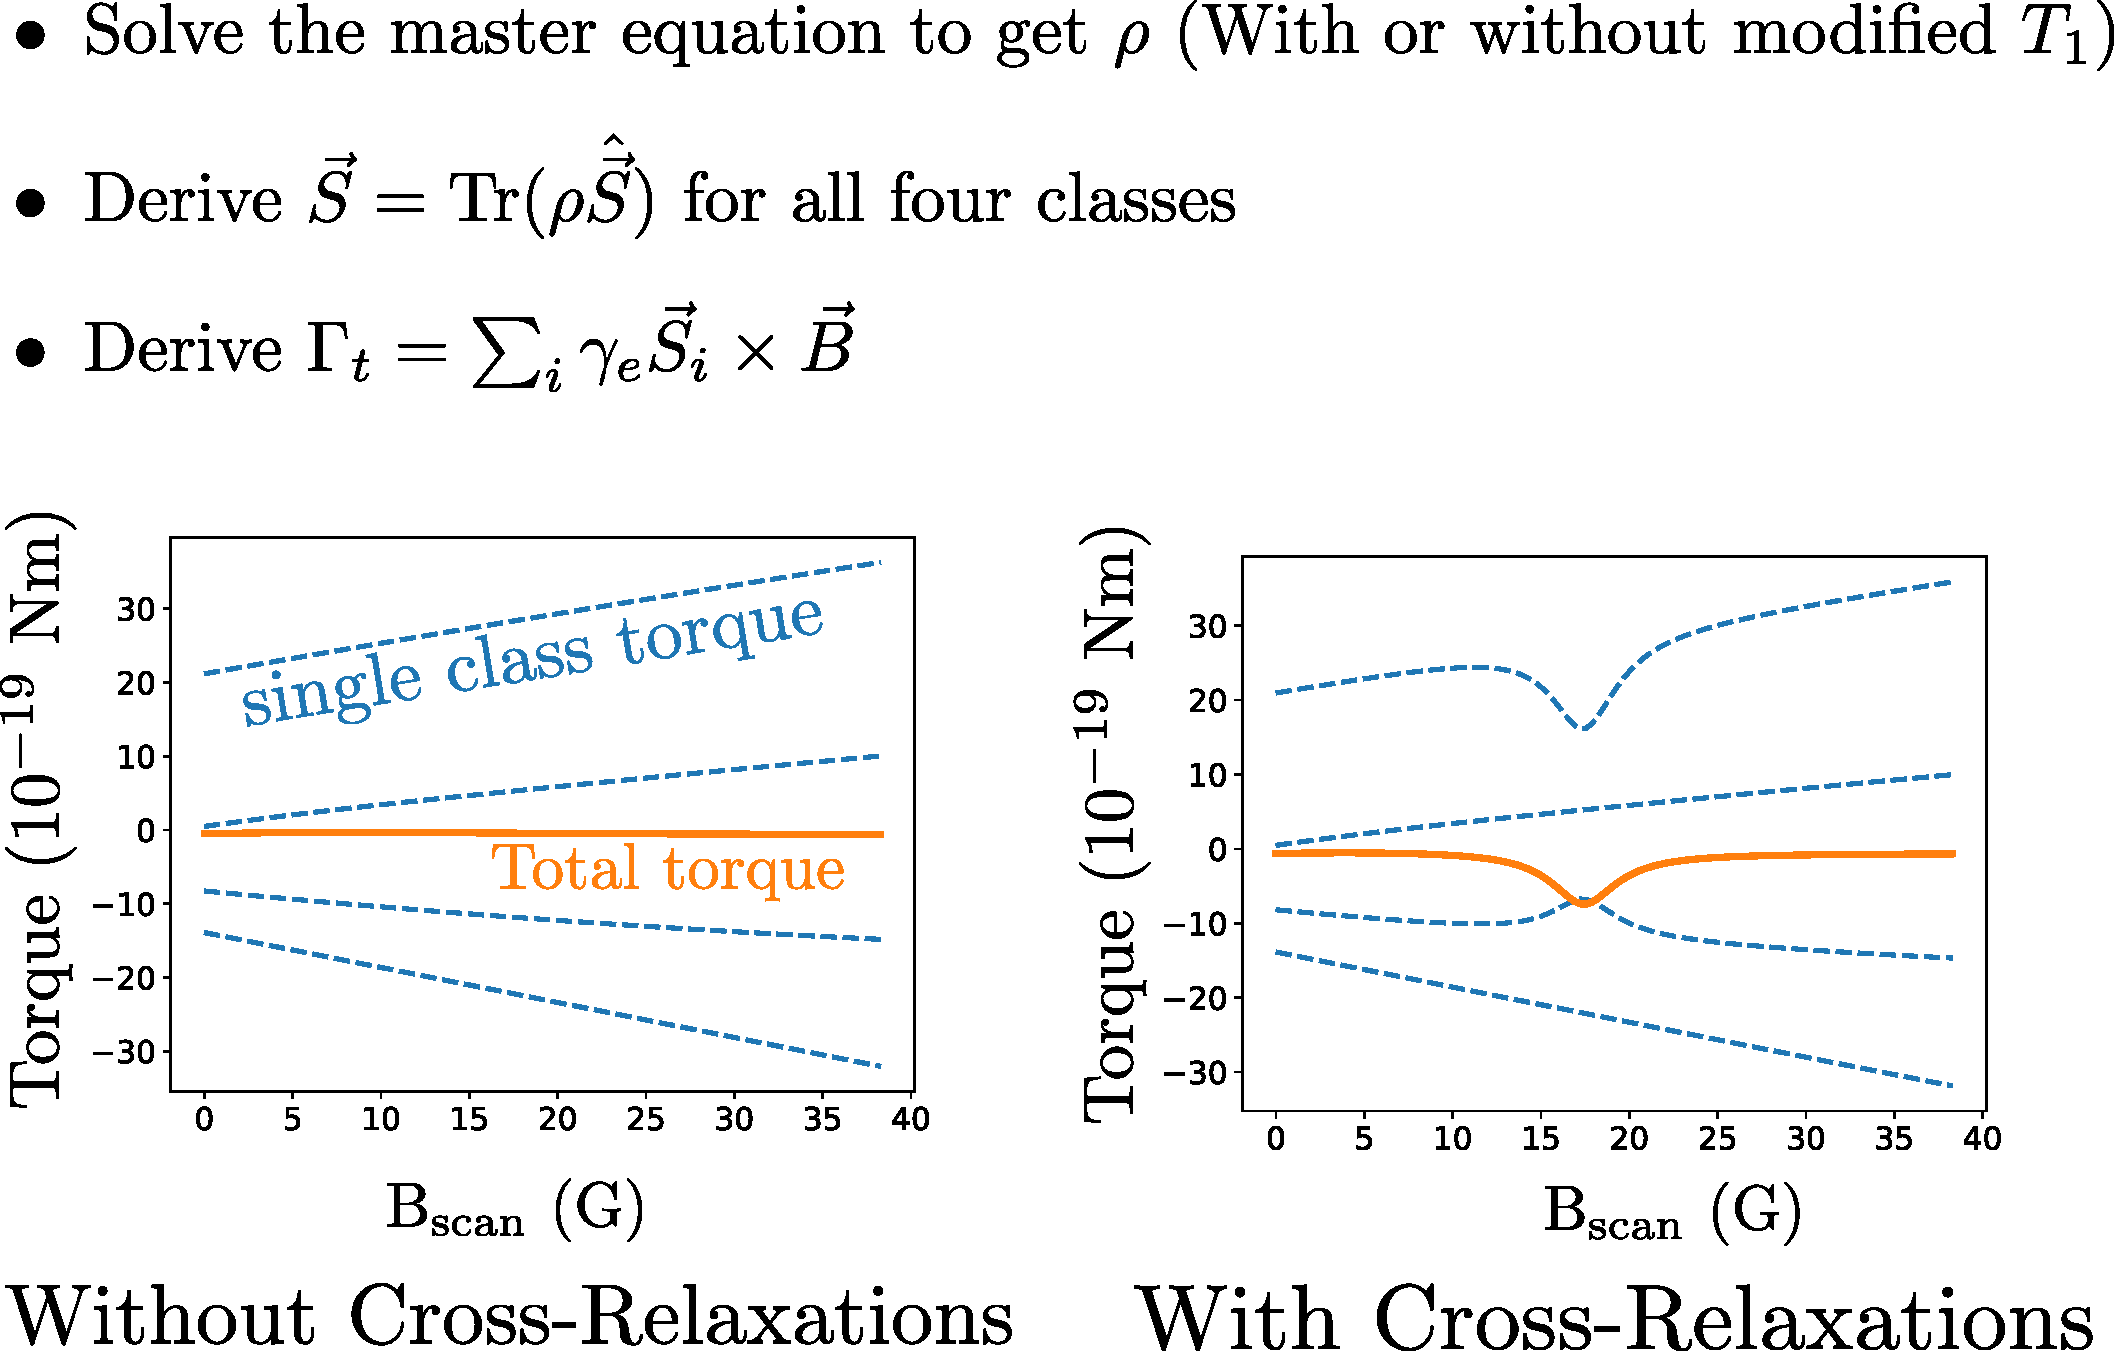
\includegraphics[scale=.3]{Explication_torque}
\end{frame}
\begin{frame}{Torque caused by CR : other configuration}
\centering
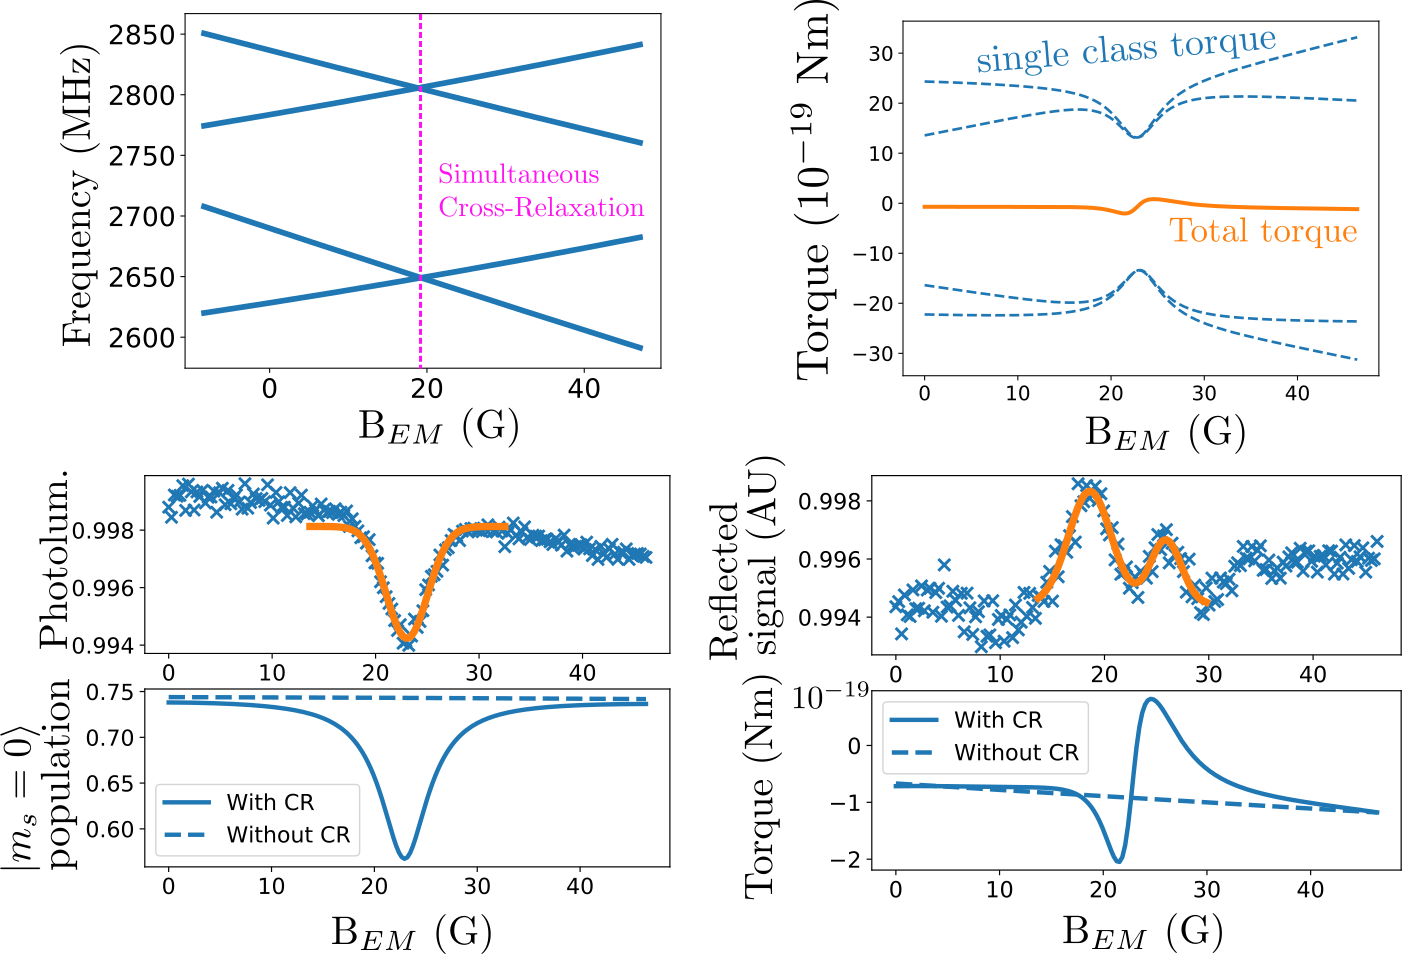
\includegraphics[scale=.28]{CRmeca_22}
\end{frame}
\begin{frame}{T1}
\centering
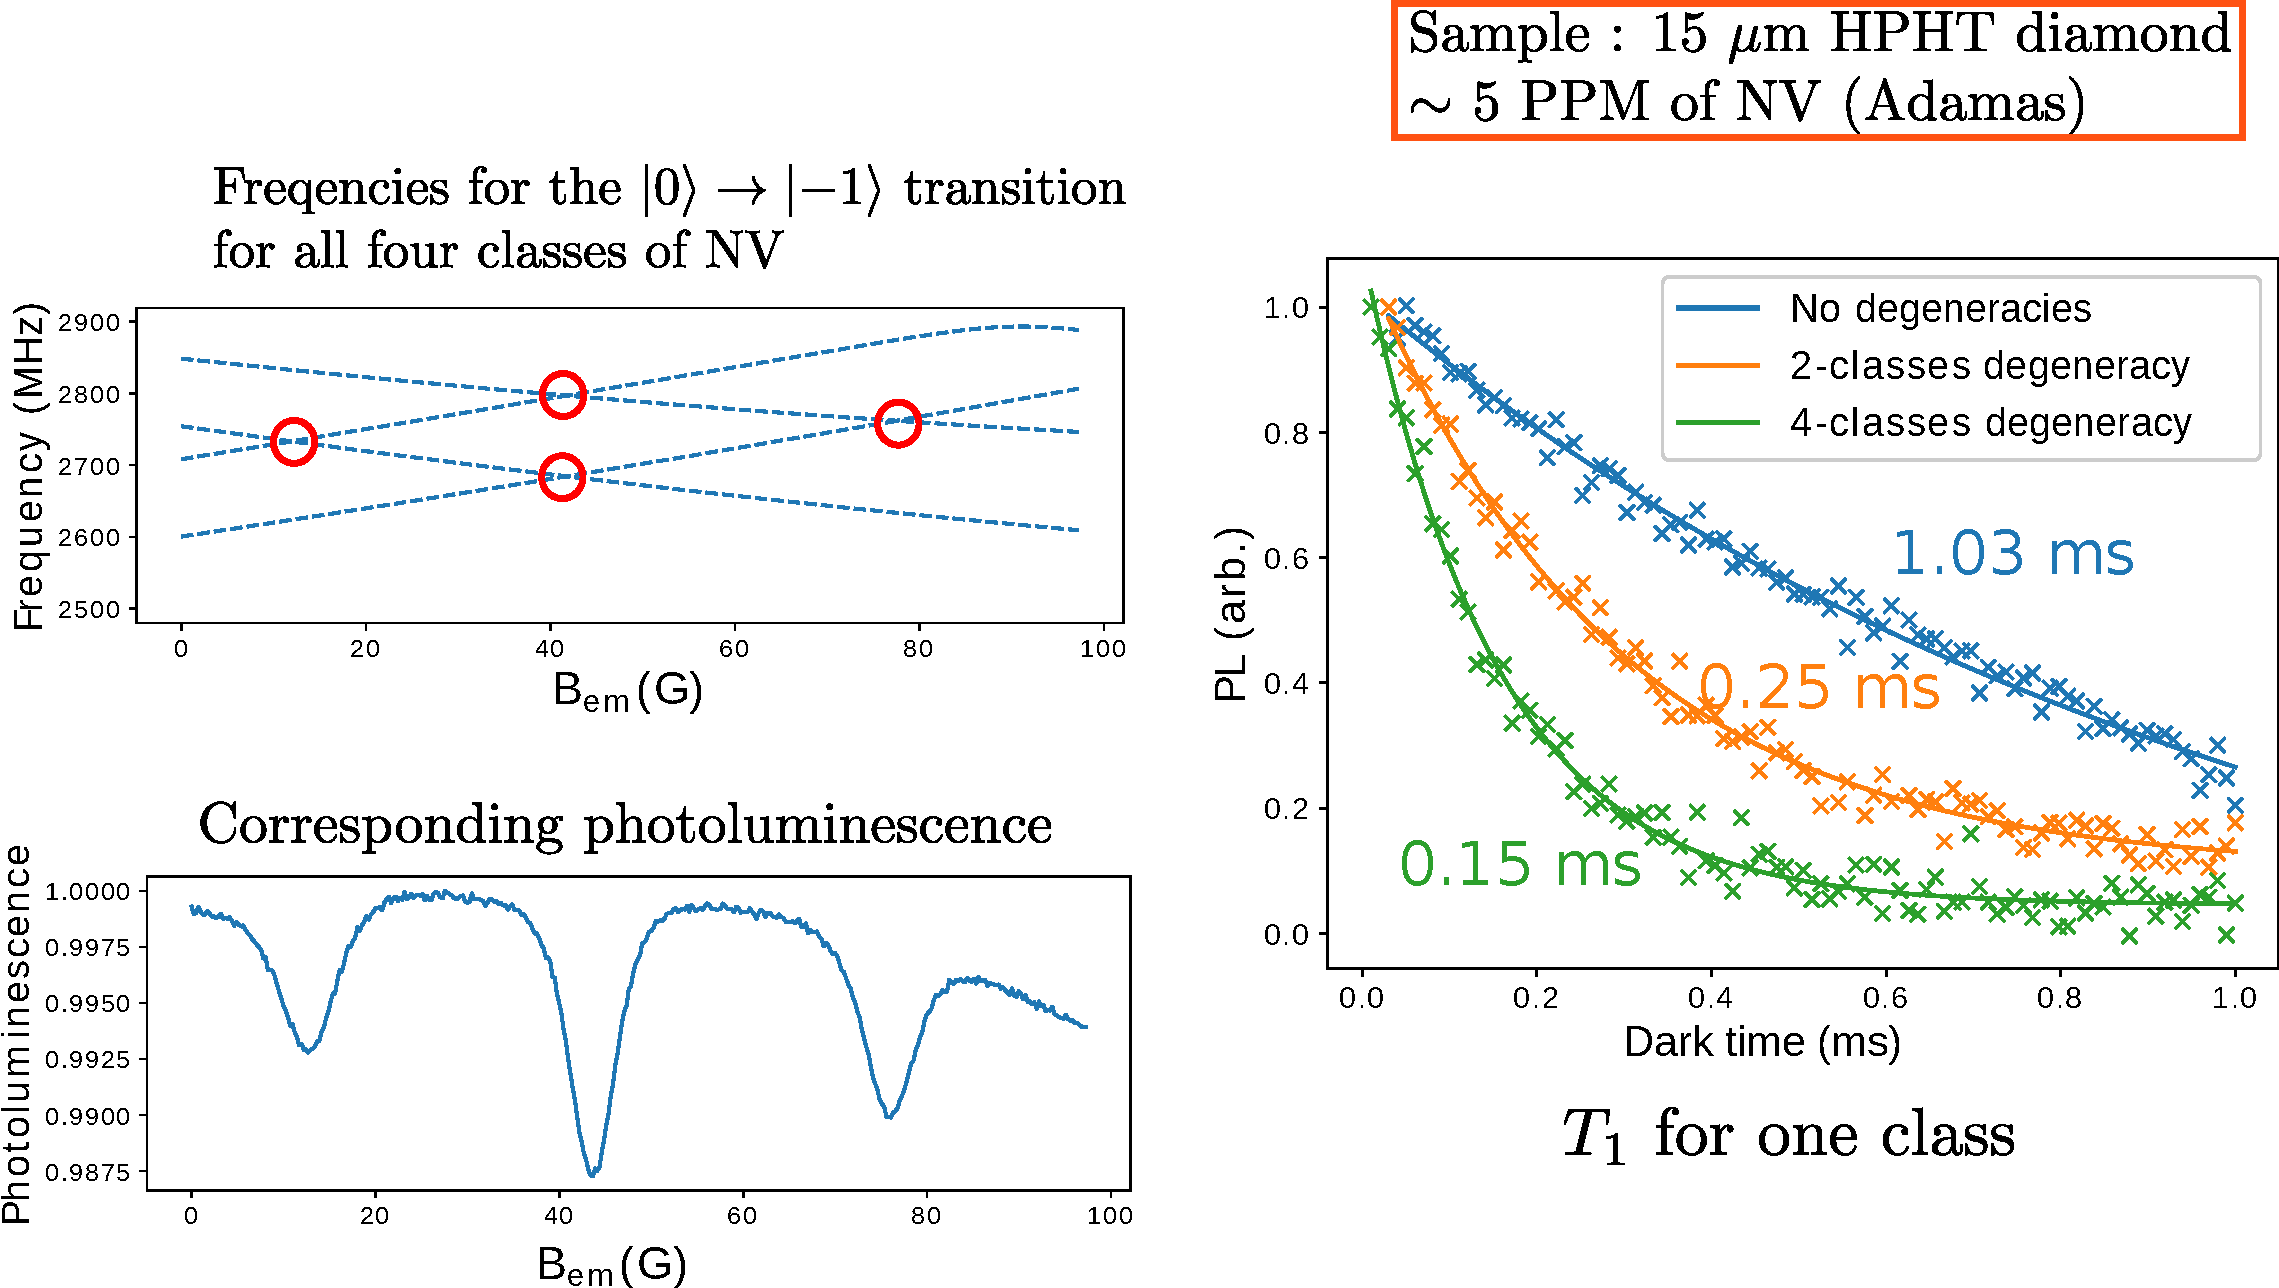
\includegraphics[scale=.28]{NV-NV_3}
\end{frame}
\end{document}